\documentclass[openany,12pt]{book}
\usepackage{datetime2}
\DTMsetdatestyle{ddmmyyyy}
\usepackage{hyperref}
\usepackage{xcolor}
\hypersetup{colorlinks=true,linkcolor=black}
\usepackage{amssymb}
\usepackage{notomath}
\usepackage[T1]{fontenc}
\usepackage[paperwidth=8.5in, paperheight=11in,inner=1.0in,outer=0.75in,top=0.75in,bottom=0.75in,twoside]{geometry} % US Letter, smaller margins
% \usepackage[paperwidth=8.5in, paperheight=11in,inner=1.5in,outer=1.0in,top=0.75in,bottom=0.75in,twoside]{geometry} % US Letter
% \usepackage[paperwidth=9.35in, paperheight=6.05in,inner=1.5in,outer=1.0in,top=0.75in,bottom=0.75in,twoside]{geometry} % 8.5 x 5.5 (scale in post process)
\usepackage{multirow}
\usepackage{graphbox}
\usepackage{sectsty}
\usepackage[Bjornstrup]{fncychap} % Bjornstrup Glenn
\usepackage{framed}
\usepackage{fancyvrb}

\definecolor{red}{rgb}{1.0, 0.0, 0.0}
\definecolor{darkblue}{rgb}{0.1, 0.0, 0.6}
\definecolor{silver}{rgb}{0.85, 0.85, 0.85}
\ChNumVar{\color{darkblue}\fontsize{55}{60}\usefont{OT1}{pzc}{m}{n}\selectfont}
\ChTitleVar{\color{darkblue}\raggedleft\LARGE\sffamily\bfseries}

\allsectionsfont{\color{darkblue}\bfseries\sffamily}

\newenvironment{note}{\begin{leftbar}{\color{red}\bf\ Note:}}{\end{leftbar}}

\newcommand{\jr}{F256}
\newcommand{\fjr}{F256jr}
\newcommand{\fk}{F256k}
\newcommand{\microsec}{$\mu$s}
\newcommand{\example}[1]{\subsection*{Example: #1}}
\begin{document}
\begin{titlepage}
    \colorbox{silver}{\makebox[\textwidth][r]{
    \shortstack{
        \vspace{3cm} \\
        \color{darkblue}\bfseries\sffamily\Huge Foenix \jr\ Reference Manual\\
        \hfill\color{darkblue}\bfseries\sffamily\Huge 6809 Big Endian Edition}} \\
    }

    \vfill

    \hfill\mbox{\color{darkblue}\bfseries\sffamily\Large Peter Weingartner}
    
    \hfill\mbox{\color{darkblue}\bfseries\sffamily\large 6809 Changes by John Federico}

    \hfill\mbox{\color{darkblue}\bfseries\sffamily\large \today}
\end{titlepage}

\tableofcontents
\listoftables

\chapter{Introduction}

This manual is meant to be a thorough introduction to the various hardware features of the \jr. In it, I will attempt to explain each of the major subsystems of the \jr\ and provide simple but practical examples of their use.

One thing this manual will not provide is a tutorial in programming the 65C02 processor at the heart of the \jr. There are plenty of excellent books and videos explaining how the processor works and how to do assembly programming. While examples will generally be written in assembly, I will try to annotate them fully so that what is happening is very clear even to the novice assembly language coder.

There are two models of \jr\ available: the \fjr, and the \fk. The \fjr\ is a single board computer, designed to fit within a mini-ITX case, that requires a separate PS/2 keyboard. The \fk\ is a complete system with a case and a built-in custom keyboard. The two versions do have differences but are mostly compatible. Differences between the systems will be clearly noted.

Several of chapters in this manual include example assembly code to show how the various features of the \jr\ work. While the code included in the text should be executable, the complete examples can be found on the Github repository that hosts the manual itself. Most of the examples are able to run on their own, but a few of them expect there to be some sort of operating system providing text display routines compatible with the old Commodore kernel. The examples were all written on a machine using OpenKERNAL, which was written for the \jr, but really anything that provides the CINT and CHROUT calls should work fine. Of course, the examples could be tweaked without too much trouble to run on essentially any operating system.

\subsection*{A Note on Notation}

Important side notes are called out with a black bar in the margin. These notes generally call out key differences between the different versions of the \jr\ and may have some important considerations for programs targeting multiple platforms.

Example code in this manual is presented as assembly language. While the code is fairly generic 65C02 assembly code, the code was tested using the 64TASS assembler, and there are aspects of its syntax that are worth explaining.

\begin{itemize}
\item Numeric literals are in decimal unless prefixed by the dollar sign (\$)
\item There are several math and logical operators that can be used to calculate a numeric literal value at assembly time: \verb|+| adds numbers, \verb+-+ subtracts, \verb+*+ multiplies, \verb+|+ calculates the bitwise OR of two values, and \verb+~+ computes the bitwise NOT or negation of a value.
\item The \verb+.byte+ directive stores a set of 8-bit values into the assembled code. The directive takes a list of values puts them into the assembled code as bytes.
\item The \verb+.word+ directive stores a set of 16-bit values into the assembled code. The directive takes a list of values and treats them as 16-bit (even if they are less than 256).
\item There are special operators for selecting specific bit ranges from a number to allow the assembly code to write the number byte-by-byte. The less than character (\verb+<+) selects bits 0--7. The greater than character (\verb+>+) selects bits 8--15. The back tick character (\verb+`+) selects bits 16--23. For example:
\end{itemize}

\begin{Verbatim}[samepage=true]
    SAMPLE = $123456

    lda #<SAMPLE
    sta $0800           ; Store $56 to $0800
    lda #>SAMPLE
    sta $0801           ; Store $34 to $0801
    lda #`SAMPLE
    sta $0802           ; Store $12 to $0802
\end{Verbatim}

\section*{About the Machine}

\subsection*{F256jr Ports}

The connectors of the back of the \fjr\ from left to right are (see figure:~\ref{fig:rear}):

\begin{description}
    \item[Audio Line Out] the stereo audio output. These are standard RCA style line level outputs.

    \item[SD Card Slot] for standard SD cards for storage of files and programs.

    \item[DVI Monitor Port] for output to your monitor. This can be connected to the DVI input of a monitor or run through a simple DVI-VGA connector to use with an older VGA input.

    \item[IEC Serial Port] supports the Commodore serial bus. A Commodore disk drive (1541, 1571, 1581, {\it etc.}), a Commodore compatible serial printer, or other device supporting the Commodore serial bus can be connected here.
\end{description}

\begin{figure}[ht]
    \begin{center}
        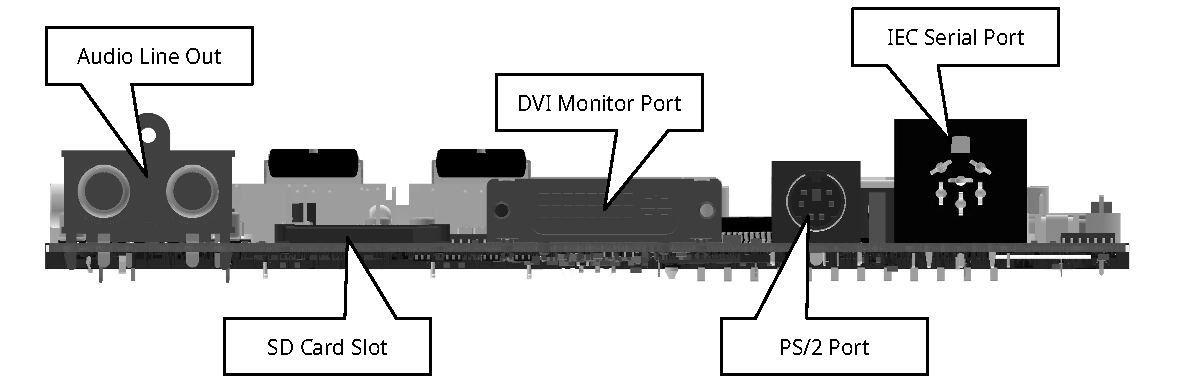
\includegraphics[scale=0.75]{images/f256_render_annotated_back.pdf}
    \end{center}
    \caption{F256jr Rear Connectors}
    \label{fig:rear}
\end{figure}


The top of the \fjr\ board has several connectors and other features that should be explained (see figure:~\ref{fig:top}):

\begin{description}
    \item[Power In] this is a standard ITX/ATX style power connector. Pretty much any PC power supply should work here, and a Pico-ATX style power adapter is more than sufficient.

    \item[Debug USB Port] this provides access to the debug interface of the \jr\ for a desktop computer. You can use it to upload data to the \jr's memory or examine the memory. There is a Mini USB B connector on the board, but there is also a header that can be used to connect the USB jack on some cases to the board.

    \item[Case Buttons and LEDs] this collection of headers is used to connect the power and reset button from the case as well as the power LED and SD access LED.

    \item[Joystick Ports] these connectors allow you to plug in Atari style joysticks

    \item[DIP Switches] these switches allow you to manage certain aspects of the \jr. In particular, you can control gamma correction and some boot options, depending on the kernel installed.

    \item[Stereo SIDs] out of the box, these will be bare sockets, but they are where you would install your SID chips or SID emulators. The sockets support the original 6581, the lower voltage 8581, and the different replacements like the SwinSID, ARMSID, and BackSID.

    \item[Wi-Fi Module] this optional module works with the built-in serial port to allow for Wi-Fi access, if a program or operating system supports it.

    \item[RS-232 Port] this IDC header works with a standard IDC to DE-9 adapter cable to provide an RS-232 serial port. The same serial port is used for this port as is used by the Wi-Fi module, so only one of the two can be used at a time.

    \item[GPIO] this header provides access to the I/O pins of the WDC65C22 VIA. The pin assignments are compatible with the Commodore C64 keyboard connector.

    \item[Expansion Port] for future expansion. This is a PCI-E style connector with a custom pinout. In the future, it might be used for memory expansion or other devices.

    \item[Clock Battery] this CR2032 cell holder provides power for the real time clock chip.

    \item[FPGA JTAG Port] this connector is used to apply any future updates to the FPGA. A special adapter would need to be used to connect to this port.

    \item[Gamepad Ports] this header provides access for an NES or SNES style gameport interface.

    \item[Case Audio Port] this header provides access to the headphone and microphone signals to connect to a PC case.

    \item[Headphone Out] this is a standard headphone adapter port that can be used if the case does not provide headphone output.
\end{description}

\begin{figure}[ht]
    \begin{center}
        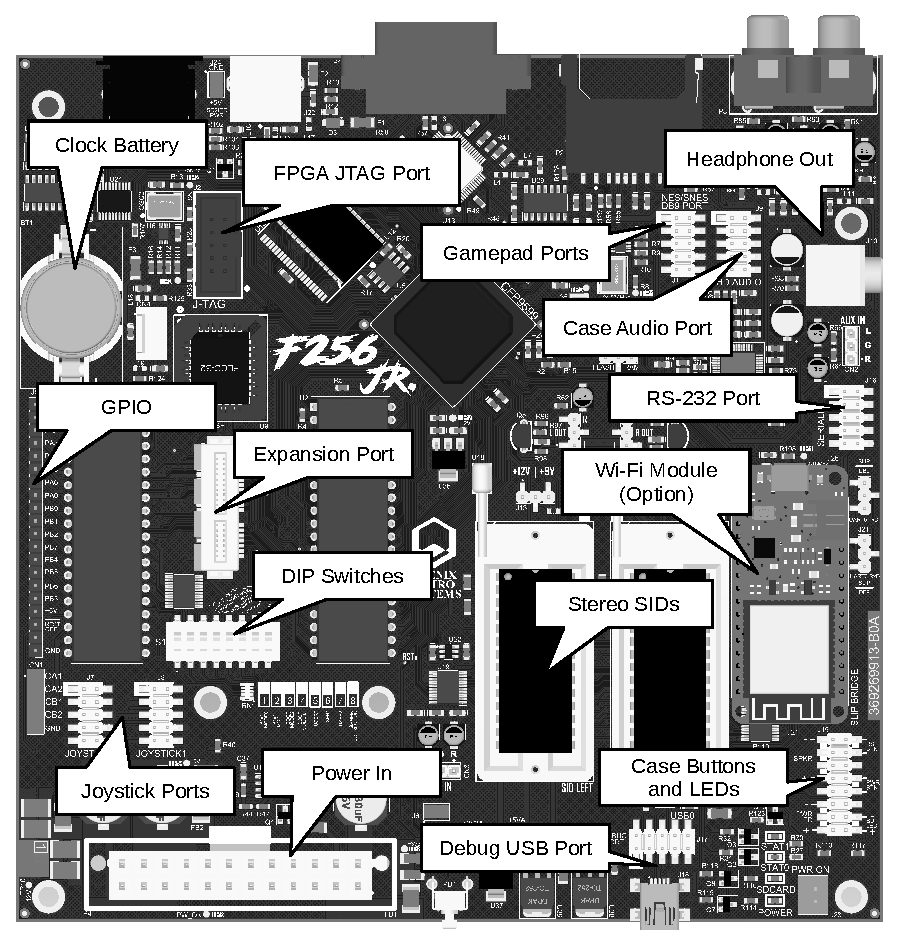
\includegraphics[scale=0.55]{images/f256_render_annotated_top.pdf}
    \end{center}
    \caption{F256jr Top View}
    \label{fig:top}
\end{figure}

\subsection*{F256k Ports}

The connectors of the back of the \fk\ from left to right are (see figure:~\ref{fig:rear_k}):

\begin{description}
	\item[Power Jack] The \fk\ requires a 12 volt DC power supply that can provide at least 2 amps. They are available from several suppliers and should be readily available. The connector needed is a 2.5mm barrel plug with a center-positive connection ({\it i.e.} the outer sleave is ground).
	
	\item[USB Debug Port] provides the debug interface through USB
    
    \item[PS/2 Mouse Port] provides the PS/2 interface for a mouse
    
    \item[FNX4N4S Adapter Port] provides the connections for NES style gamepads, through FNX4N4S adapter module
    
    \item[IEC Serial Port] supports the Commodore serial bus. A Commodore disk drive (1541, 1571, 1581, {\it etc.}), a Commodore compatible serial printer, or other device supporting the Commodore serial bus can be connected here.

    \item[DVI Monitor Port] for output to your monitor. This can be connected to the DVI input of a monitor or run through a simple DVI-VGA connector to use with an older VGA input.
    
    \item[RS-232 Port] provides a standard RS-232 serial interface
    
    \item[Headphone Port] a standard jack for headphones

    \item[Audio Line Out] the stereo audio output. These are standard RCA style line level outputs.
\end{description}

\begin{figure}[ht]
    \begin{center}
        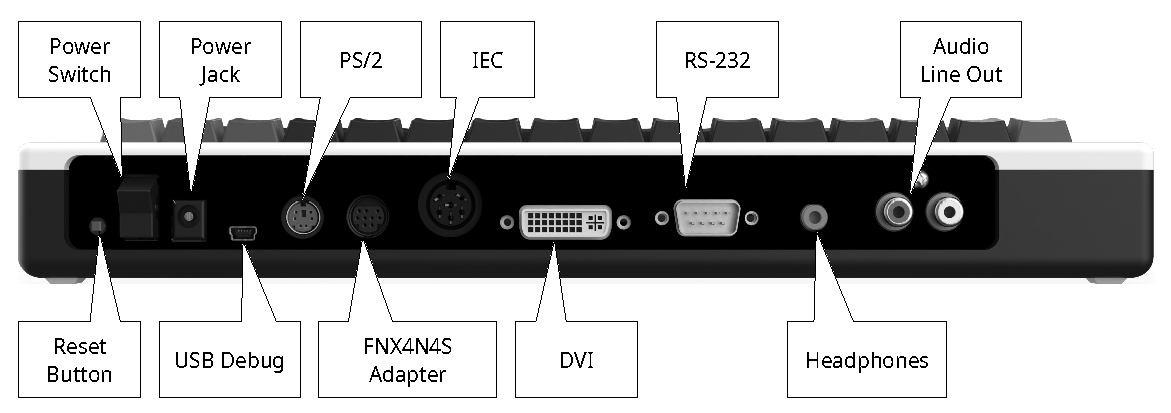
\includegraphics[scale=0.75]{images/f256k_back_annotated.pdf}
    \end{center}
    \caption{F256k Rear Connectors}
    \label{fig:rear_k}
\end{figure}

The top of the \fk\ board contains a few connectors and jumpers (see figure~\ref{fig:top_k}). Note that, for the \fk, the JTAG port and DIP switches that are on top of the \fjr\ board are on the bottom side of the \fk, and they are accessible without removing the board from the case.

\begin{description}
    \item[Audio Line-input] this three pin header provides an stereo audio line level input for the CODEC.
    
    \item[Wi-Fi Module] this optional module works with the built-in serial port to allow for Wi-Fi access, if a program or operating system supports it.

    \item[Serial Device Selectors] these two three pin headers allow the system to use either the RS-232 port on the back of the board for serial I/O or the optional Wi-Fi module.

    \item[Expansion Port] for future expansion. This is a PCI-E style connector with a custom pinout. In the future, it might be used for memory expansion or other devices.

    \item[Clock Battery] this CR2032 cell holder provides power for the real time clock chip.
    
    \item[Atari Style Joysticks] two DE-9 connectors (accessible through the side of the case) provide access for Atari style joysticks.
   \end{description}

\begin{figure}[ht]
    \begin{center}
        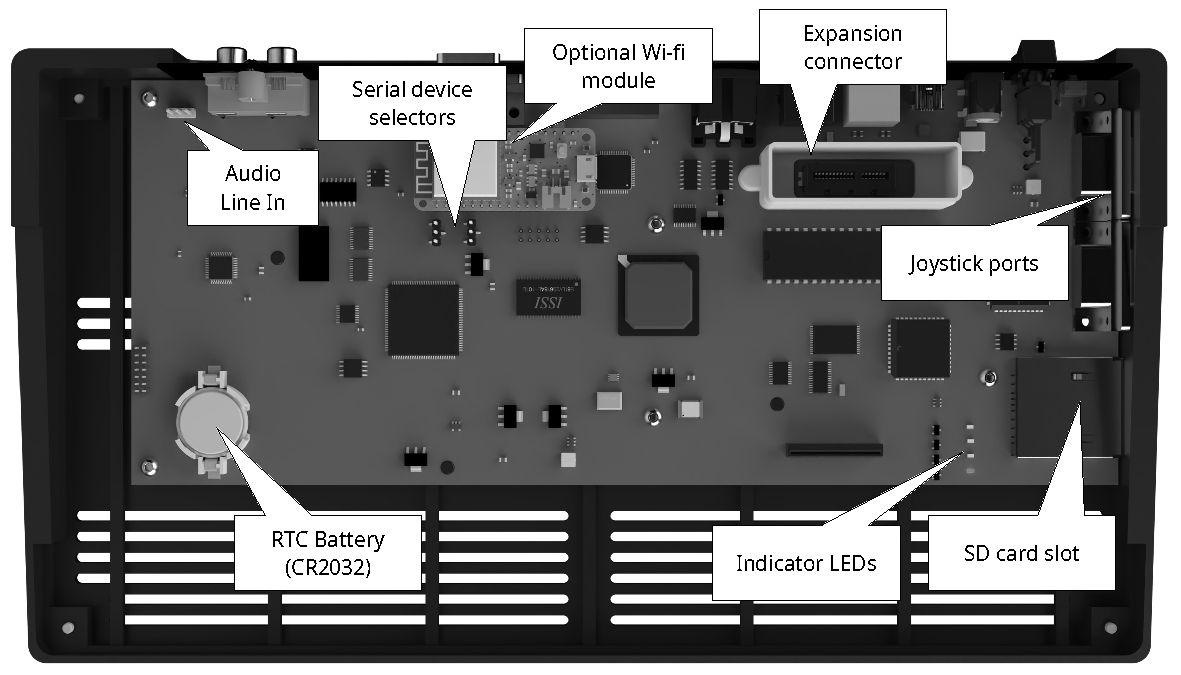
\includegraphics[scale=0.55]{images/f256k_top_annotated.pdf}
    \end{center}
    \caption{F256k Top View}
    \label{fig:top_k}
\end{figure}

\subsection*{System Architecture}

For being so small, the \jr\ has a lot of components to it, so it is worth mapping out the over all structure of the computer. One of the main things to note is that most of what makes the \jr\ the \jr\ is the FPGA TinyVicky. TinyVicky provides the MMU, the various text and graphics engines, most of the I/O devices, controllers for the sound chips, and the controller for the 512KB of SRAM. The CPU, VIA, RTC, flash memory, and expansion RAM are separate from TinyVicky, although TinyVicky is still responsible for translating CPU addresses to the appropriate chip selection logic and bank selection. One of the most important aspects of this architecture is that, while the first 512KB of SRAM is accessible to both the CPU and TinyVicky, TinyVicky cannot access the data in the flash or in any expansion RAM.

\begin{figure}[ht]
    \begin{center}
        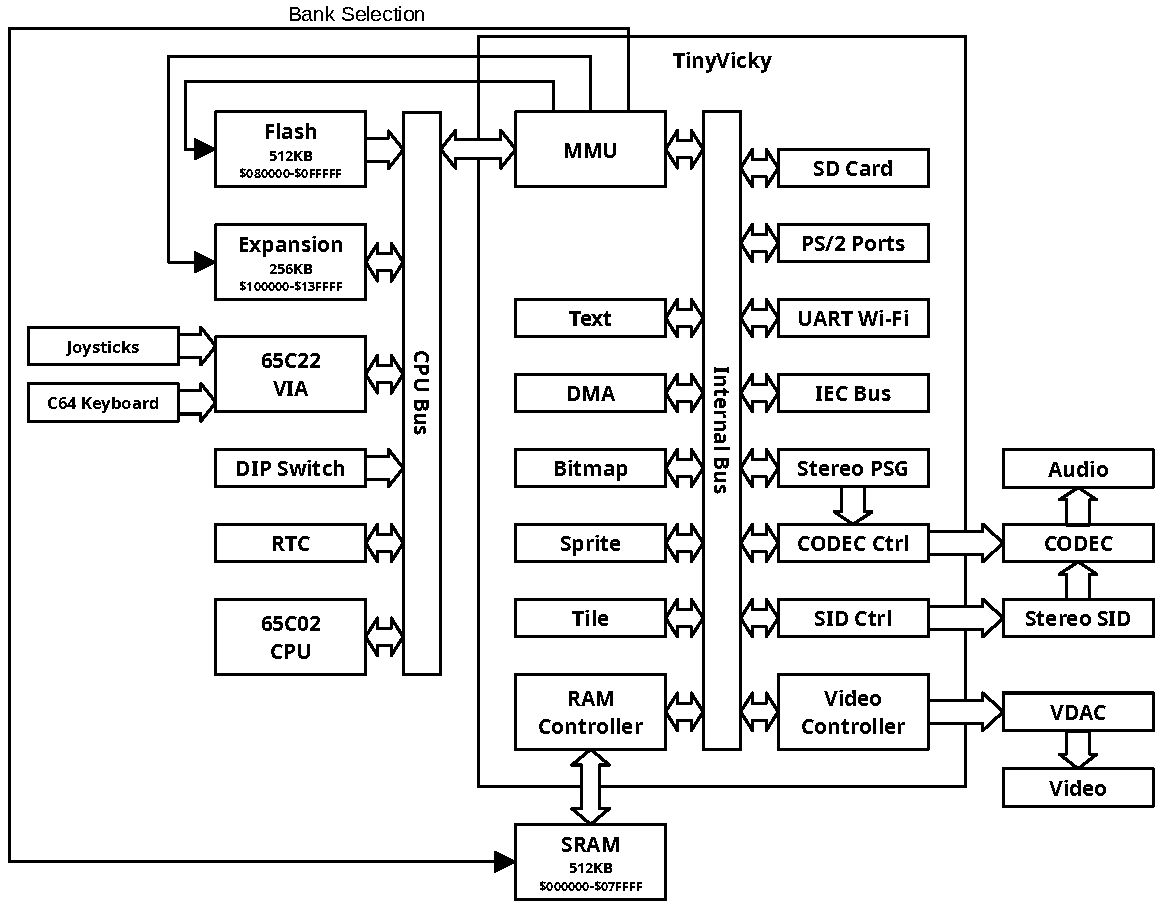
\includegraphics[scale=0.55]{images/f256jr_layout.pdf}
    \end{center}
    \caption{F256jr Internal Architecture}
    \label{fig:arch}
\end{figure}

\begin{figure}[ht]
    \begin{center}
        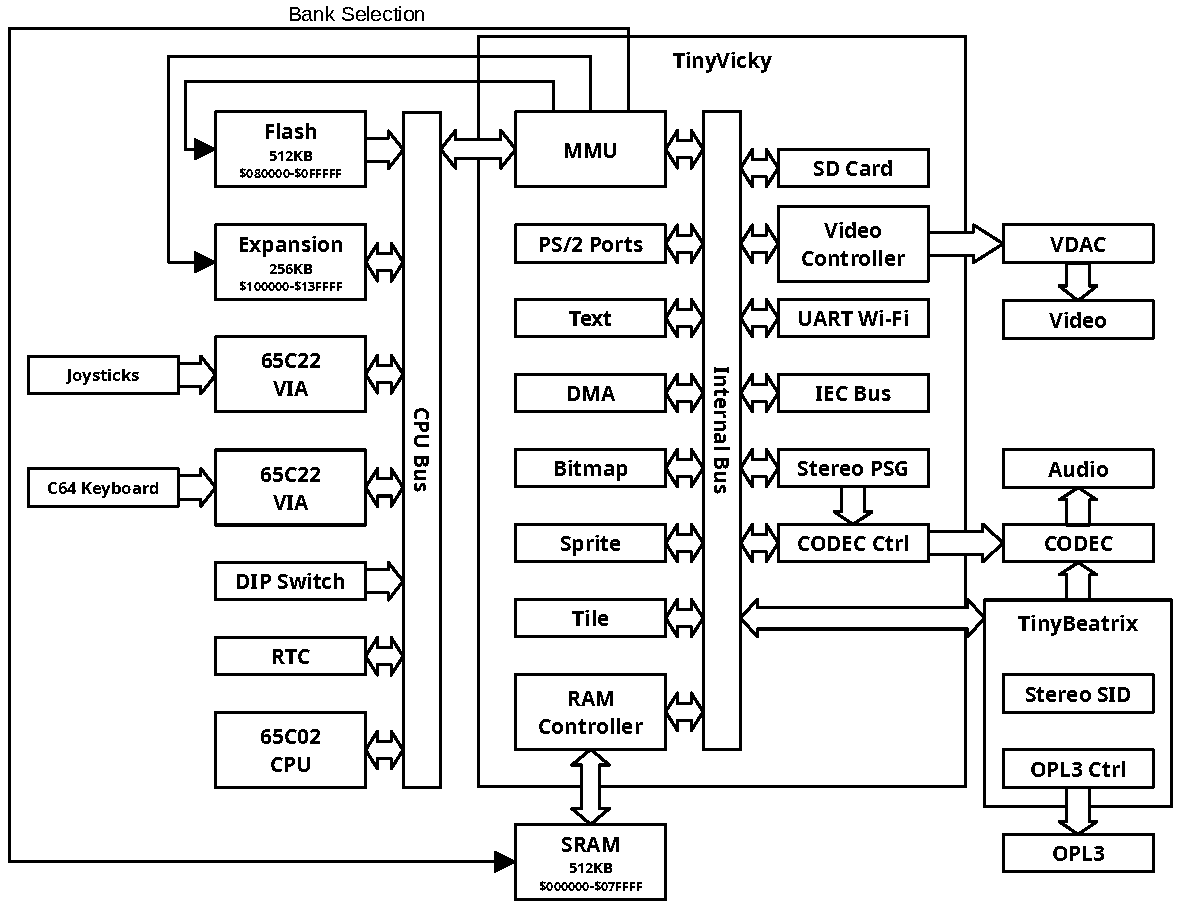
\includegraphics[scale=0.55]{images/f256k_layout.pdf}
    \end{center}
    \caption{F256k Internal Architecture}
    \label{fig:f256k_arch}
\end{figure}

\chapter{Memory Management}

The \jr\ has 256 KB of system RAM which can be used for programs, data, and graphics. It also has 512 KB of read-only flash memory that can be used by whatever operating system is installed. Now, the 65C02 CPU at the heart of the \jr\ has an address space of only 64 KB, so how can it access all this memory, not to mention the I/O devices on the system? The answer is paging. The \jr\ has a special memory management unit (MMU) that can swap banks of memory or I/O registers into and out of the memory space of the CPU.

To understand how it all works, we first need to look at how RAM and flash memory are handled by the \jr. Because there are 768 KB of total storage on the system, the system has a 20-bit address bus to manage the memory. RAM and flash have address on that 20-bit bus as shown in table~\ref{tab:memory}.

\begin{table}[h]
	\begin{center}
		\begin{tabular}{| l | l | l |} \hline
			Start & End & Memory Type \\ \hline\hline
		  	\verb+0x00000+ & \verb+0x3FFFF+ & System RAM (256 KB)\\ \hline
			\verb+0x40000+ & \verb+0x7FFFF+ & Reserved for future use (256 KB)\\ \hline
		  	\verb+0x80000+ & \verb+0xFFFFF+ & Flash Memory (512 KB) \\ \hline
		\end{tabular}
	\end{center}
	\caption{C256jr memory layout}
	\label{tab:memory}
\end{table}

This memory is divided up into ``banks'' of 8 KB each. The 16-bit address space of the CPU is also divided up into 8 KB banks. The MMU allows the program to assign any bank of system memory to any bank of the CPU's memory. It does this through the use of memory look-up tables (LUT), which provide the upper bits needed to select the bank out of system memory for any given bank in CPU memory. It takes 13 bits to specify an address within 8 KB, which means for a 16-bit address from the CPU, the upper 3 bits are the bank number. Since the system bus is 20 bits, a bank number there is 7 bits. So a LUT must provide a 7-bit system bank number for each 3-bit bank number provided by the CPU.

The \jr's MMU supports up to four LUTs, only one of which is active at any given moment. This allows programs to define four different memory layouts and switch between them quickly, without having to alter a LUT on the fly.

\begin{table}[h]
	\begin{center}
		\begin{tabular}{| c | c || c | c | c | c | c | c | c | c |} \hline
			Bank & A[15..13] & Start & End \\ \hline\hline
			0 & 000 & \verb+0x0000+ & \verb+0x1FFF+ \\ \hline
			1 & 001 & \verb+0x2000+ & \verb+0x3FFF+ \\ \hline
			2 & 010 & \verb+0x4000+ & \verb+0x5FFF+ \\ \hline
			3 & 011 & \verb+0x6000+ & \verb+0x7FFF+ \\ \hline
			4 & 100 & \verb+0x8000+ & \verb+0x9FFF+ \\ \hline
			5 & 101 & \verb+0xA000+ & \verb+0xBFFF+ \\ \hline
			6 & 110 & \verb+0xC000+ & \verb+0xDFFF+ \\ \hline
			7 & 111 & \verb+0xE000+ & \verb+0xFFFF+ \\ \hline
		\end{tabular}
	\end{center}
	\caption{CPU Memory Banks}
	\label{tab:mem_banks}
\end{table}

Of the eight CPU memory banks, one is special. Bank 6 can be mapped to memory as the rest can, or it can be mapped to I/O registers, which are not memory mapped in the same way as RAM and flash. All I/O devices on the \jr\ therefore live within 0xC000 through 0xDFFF on the CPU, but only if the MMU is set to map I/O to bank 6. There is quite a lot of I/O to access on the \jr, so there are four different banks of I/O registers and memory that can be mapped to bank 6 (see table~\ref{tab:io_banks}).

\begin{table}[h]
	\begin{center}
		\begin{tabular}{| l | l |} \hline
			I/O Bank & Purpose \\ \hline\hline
			0 & Low level I/O registers \\ \hline
			1 & Text display font memory and graphics color LUTs \\ \hline
			2 & Text display character matrix \\ \hline
			3 & Text display color matrix \\ \hline
		\end{tabular}
	\end{center}
	\caption{I/O Banks}
	\label{tab:io_banks}
\end{table}

The MMU is controlled through two main registers, which are always at locations 0x0000 and 0x0001 in the CPU's address space (see table~\ref{tab:mmu_registers}). These registers allow programs to select an active LUT, edit a LUT, and control bank 6:

\begin{table}[h]
	\begin{center}
		\begin{tabular}{| c | c | c || c | c | c | c | c | c | c | c |} \hline
			Address & R/W & Name & 7 & 6 & 5 & 4 & 3 & 2 & 1 & 0 \\ \hline\hline
			\verb+0x0000+ & RW & MMU\_MEM\_CTRL & EDIT\_EN & --- & \multicolumn{2}{|c|}{EDIT\_LUT} & --- & --- & \multicolumn{2}{|c|}{ACT\_LUT} \\ \hline
			\verb+0x0001+ & RW & MMU\_IO\_CTRL & \multicolumn{5}{|c|}{---} & IO\_DISABLE & \multicolumn{2}{|c|}{IO\_PAGE} \\ \hline
		\end{tabular}
	\end{center}
	\caption{MMU Registers}
	\label{tab:mmu_registers}
\end{table}

\begin{description}
	\item[ACT\_LUT] these two bits specify which LUT (0 - 3) is used to translate CPU bus address to system bus addresses.

	\item[EDIT\_EN] if set (1), this bit allows a LUT to be edited by the program, and memory addresses 0x0010 - 0x0017 will be used by the LUT being edited. If clear (0), those memory locations will be standard memory locations and will be mapped like the rest of bank 0.

	\item[EDIT\_LUT] if EDIT\_EN is set, these two bits will specify which LUT (0 - 3) is being editted and will appear in memory addresses 0x0010 - 0x0017.

	\item[IO\_DISABLE] if set (1), bank 6 is mapped like any other memory bank. If clear (0), bank 6 is mapped to I/O memory.

	\item[IO\_PAGE] if IO\_DISABLE is clear, these two bits specify which bank of I/O memory (0 - 3) is mapped to bank 6.
\end{description}

\example{Setting up a LUT}

In this example, we will set up LUT 1 so that the first six banks of CPU memory map to the first banks of RAM, bank 7 of CPU memory maps to the first bank of flash memory, and bank 6 maps to the first I/O bank.

\begin{verbatim}
    lda #$90      ; Active LUT = 0, Edit LUT#1
    sta $0000

    ldx #0        ; Start at bank 0
l1: txa           ; First 6 banks will just be the first banks of RAM
    sta $0008,x   ; Set the LUT mapping for this bank
    inx           ; Move to the next bank
    cpx #6        ; Until we get to bank 6
    bne l1

    lda #$40      ; Bank 7 maps to $80000, first bank of flash
    sta $0017

    stz $0001     ; Bank 6 should be I/O bank 0

    lda #$01      ; Turn off LUT editting, and switch to LUT#1
    sta $0000
\end{verbatim}

\section*{MMU Boot Configuration}

While the MMU registers allow the MMU to select one of four memory LUTs to be used for address translation or to be editted, in fact the \jr's MMU actually has eight LUTs in two sets of four. At any given time, only one of those sets of four LUTs is active. One set of LUTs is the ``boot from RAM'' set, and the other is the ``boot from flash'' set. As the names imply, one set is meant to allow you to boot the \jr\ to run code you have loaded into RAM (useful for development and debugging), while the other is meant to be used to boot up an operating system you have loaded into flash memory (useful for just running programs and playing games).

When the \jr\ powers on, it initializes the LUTs in two different ways. The ``boot from RAM'' LUTs are initialized so the 64KB of CPU address space is simply mapped to the first 64KB of system RAM. The ``boot from flash'' LUTs are initialized to be the same, except that the last bank of CPU address space (0xE000 -- 0xFFFF) is mapped to the last bank of flash memory (0x7E000 -- 0x7FFFF). After the LUTs are initialized, the \jr\ checks to see which of the two sets of LUTs should be used and enables them. The memory LUTs that are not selected are completely ignored. See figure ~\ref{fig:lut_choice} to see how the LUTs are related and how they are initialized on power up.

\begin{figure}[h]
    \begin{center}
        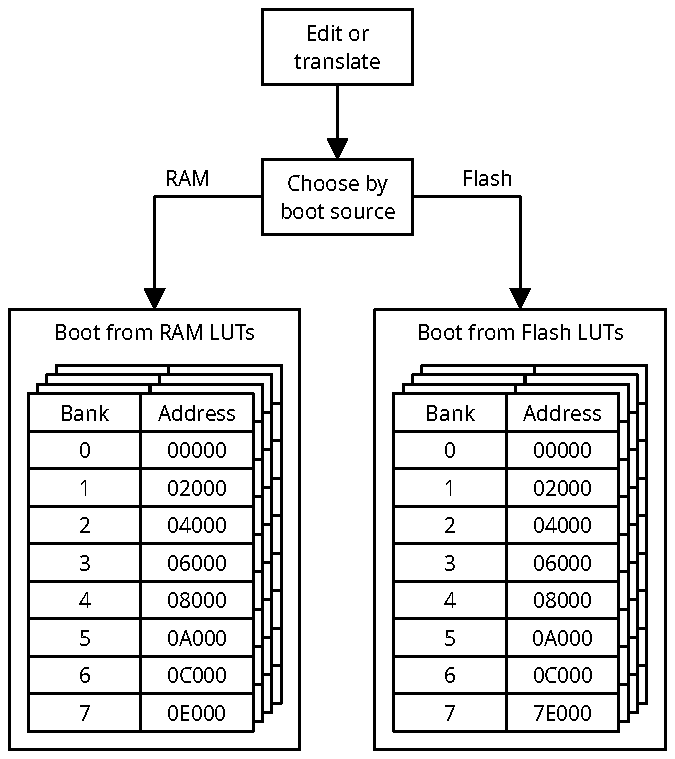
\includegraphics{images/MemoryLUTSelection.pdf}
    \end{center}
    \caption{MMU Boot Configuration}
    \label{fig:lut_choice}
\end{figure}

How the \jr\ decides which set of LUTs to use depends upon the board. The older, RevA boards have a command available over the USB debug port that switches the active LUTs on the fly. The newer, RevB boards have a jumper to choose between the LUTs.

NOTE: the memory LUTs are really just tables stored in RAM in the TinyVicky chip, and apart from the power-up initialization, TinyVicky does not change the LUTs except when directed by a program. Pressing the RESET button does not re-initialize the LUTs. This means that a program should not assume the LUTs are set to any particular value on reset, unless the operating system is initializing the LUTs. A program running as an operating system or even just taking complete control over the board should always iniitalize the LUTs to the values it needs as one of its first tasks. Of course, a complete power cycle of the board will reset the LUTs, but a program will not always be starting from a complete power cycle.

\chapter{The Text Screen}

The display on the \jr\ is managed by TinyVicky, which is the smaller member of the Vicky family of display controllers in the other Foenix machines. TinyVicky provides several display engines to let your programs control the screen:

\begin{itemize}
    \item Text: an old school style text screen where the characters to display are stored in a text matrix, and the shape of those characters comes from font memory. Text mode characters are 8 pixels wide by 8 pixels high.
    \item Bitmap: a simple pixel graphics mode that can be either 300x240 or 300x200.
    \item Sprite: an engine to display small, movable sprites on the screen.
    \item Tile: an engine to display images on the screen made up of tiles from a tile set.
\end{itemize}

The bitmap, sprite, and tile engines are considered graphics modes. TinyVicky will let you display either text by itself, a mix of the graphics modes by themselves, or text overlaid on top of the graphics modes.

\section*{Text Matrix}

The memory for the characters to display on the screen is the text matrix, which is stored in I/O page 2. When this I/O page is swapped into the CPU address space, it appears at 0xC000. Each byte of memory corresponds to a single character on the screen in left to right, top to bottom order. The byte at 0xC000 is the upper left corner of the screen, the byte at 0xC001 is the next character to the right, and so on. The number of bytes per line is set by the base resolution of the screen, but is generally 80. When a border is displayed, while that limits the number of characters displayed, the layout in memory remains the same.

The text screen has two core resolutions, tied to the refresh rate of the screen: 80 by 60 at 60 Hz, and 80 by 50 at 70 Hz. Beyond that, the character display may be made double width or double height, or both. This gives the following possible character displays: $80 \times 60$, $40 \times 60$, $80 \times 30$, $40 \times 30$, $80 \times 50$, $40 \times 50$, $80 \times 25$, and $40 \times 25$.

\example{Print an A to the Screen}
\begin{verbatim}
    lda $0001       ; Save the current MMU setting
    pha

    lda #$02        ; Swap I/O Page 2 into bank 6
    sta $0001

    lda #'A'        ; Write 'A' to the upper left corner
    sta $C000

    pla             ; Restore the old MMU setting
    sta $0001
\end{verbatim}

Note: this example does not set the font or the color, so depending on how your \jr\ is initialized, you may not see an actual ``A'' on the screen.

\section*{Text Color LUTs}

Characters in TinyVicky text mode have two colors: the foreground and the background. The foreground and background colors are picked for each character out of two different palettes of 16 colors each. The colors in the palettes are picked from the full range of colors \jr\ can produce, which is more than 16 million colors. This is all managed through two color lookup tables (LUTs) provided by TinyVicky: a text foreground color LUT, and a text background color LUT.

The text LUTs are stored in I/O page 0. The foreground LUT starts at 0xD800, and the background LUT starts at 0xD840.

Each LUT is a list of 16 entries. Each entry is a set of four bytes: blue, green, red, and alpha. Each byte indicates how much of that primary color is present as a component of the actual color. The values range from 0 (none) to 255 (as much as possible). Currently, the alpha channel is not used and is there for future expansion.

\begin{table}[ht]
    \begin{center}
        \begin{tabular}{|c|c|c|c|c|c|c|c|} \hline
            Index & R/W & Foreground & Background & 0 & 1 & 2 & 3 \\ \hline\hline
            0 & W & \verb+0xD800+ & \verb+0xD840+ & BLUE\_0 & GREEN\_0 & RED\_0 & X \\ \hline
            1 & W & \verb+0xD804+ & \verb+0xD844+ & BLUE\_1 & GREEN\_1 & RED\_1 & X \\ \hline
            2 & W & \verb+0xD808+ & \verb+0xD848+ & BLUE\_2 & GREEN\_2 & RED\_2 & X \\ \hline
            3 & W & \verb+0xD80C+ & \verb+0xD84C+ & BLUE\_3 & GREEN\_3 & RED\_3 & X \\ \hline
            4 & W & \verb+0xD810+ & \verb+0xD850+ & BLUE\_4 & GREEN\_4 & RED\_4 & X \\ \hline
            5 & W & \verb+0xD814+ & \verb+0xD854+ & BLUE\_5 & GREEN\_5 & RED\_5 & X \\ \hline
            6 & W & \verb+0xD818+ & \verb+0xD858+ & BLUE\_6 & GREEN\_6 & RED\_6 & X \\ \hline
            7 & W & \verb+0xD81C+ & \verb+0xD85C+ & BLUE\_7 & GREEN\_7 & RED\_7 & X \\ \hline
            8 & W & \verb+0xD820+ & \verb+0xD860+ & BLUE\_8 & GREEN\_8 & RED\_8 & X \\ \hline
            9 & W & \verb+0xD824+ & \verb+0xD864+ & BLUE\_9 & GREEN\_9 & RED\_9 & X \\ \hline
            10 & W & \verb+0xD828+ & \verb+0xD868+ & BLUE\_10 & GREEN\_10 & RED\_10 & X \\ \hline
            11 & W & \verb+0xD82C+ & \verb+0xD86C+ & BLUE\_11 & GREEN\_11 & RED\_11 & X \\ \hline
            12 & W & \verb+0xD830+ & \verb+0xD870+ & BLUE\_12 & GREEN\_12 & RED\_12 & X \\ \hline
            13 & W & \verb+0xD834+ & \verb+0xD874+ & BLUE\_13 & GREEN\_13 & RED\_13 & X \\ \hline
            14 & W & \verb+0xD838+ & \verb+0xD878+ & BLUE\_14 & GREEN\_14 & RED\_14 & X \\ \hline
            15 & W & \verb+0xD83C+ & \verb+0xD87C+ & BLUE\_15 & GREEN\_15 & RED\_15 & X \\ \hline
        \end{tabular}
    \end{center}
    \caption{Text Color Lookup Tables}
    \label{tab:text_luts}
\end{table}

\section*{Color Matrix}

The way that text color is selected for each character is through the color matrix. This section of memory is in I/O page 3 and starts at 0xC000 when page 3 is swapped into the CPU's address space. The layout is precisely the same as the text matrix (e.g. the character at 0xC123 in the text matrix has its color information at 0xC123 in the color matrix).

Each byte in the color matrix specifies two colors by providing an index into each of the two text LUTs. The most significant four bits is the number of the foreground color to use. The number of the least significant four bits is the number of the background color to use.

Let's say the color value at 0xC123 is 0x45. This means that the foreground color of the character is color 4 from the text foreground LUT, which starts at 0xD810 (0xD800 + 4 * 4), and the background color of the character is 5 from the text background LUT, which starts at 0xD854 (0xD840 + 4 * 5). If the bytes at 0xD810 are 0x00, 0x80, 0x80, that means the foreground will be a medium yellow. If the bytes at 0xD854 are 0xFF, 0x00, 0x00, that means the background will be blue.

\example{Make That ``A'' Yellow on Blue}
\begin{verbatim}
    lda $0001       ; Save the MMU state
    pha

    stz $0001       ; Switch in I/O Page #0

    stz $D810       ; Set foreground #4 to medium yellow
    lda #$80
    sta $D811
    sta $D812

    lda #$FF        ; Set background #5 to blue
    sta $D854
    stz $D855
    stz $D856

    lda #$03        ; Switch to I/O page #3 (color matrix)
    sta $0001

    lda #$45        ; Color will be foreground=4, background=5
    sta $C000

    pla             ; Restore the MMU state
    sta $0001
\end{verbatim}

\section*{Entering Text Mode}

Whether text mode is being displayed (and in what resolution) is controlled by the VICKY Master Control Registers (see table~\ref{tab:vky_master_ctrl_reg}). For now, we're going to ignore most of the bits, which are used by other display modes. For text mode, we really only care about the TEXT bit, which needs to be set to turn on the text display. The resolution is controlled by DBL\_Y, DBL\_X, and CLK\_70. If we set 0xD000 to 0x01 and 0xD001 to 0x00, that will put us into text mode at $80 \times 60$.

\begin{table}[ht]
    \begin{center}
        \begin{tabular}{|c|c|c|c|c|c|c|c|c|c|} \hline
            Address & R/W & 7 & 6 & 5 & 4 & 3 & 2 & 1 & 0 \\ \hline\hline
            \verb+0xD000+ & R/W & X & GAMMA & SPRITE & TILE & BITMAP & GRAPH & OVRLY & TEXT \\ \hline
            \verb+0xD001+ & R/W & \multicolumn{2}{|c|}{---} & FON\_SET & FON\_OVLY & MON\_SLP & DBL\_Y & DBL\_X & CLK\_70 \\ \hline
        \end{tabular}
    \end{center}
    \caption{VICKY Master Control Registers}
    \label{tab:vky_master_ctrl_reg}
\end{table}

\begin{description}
    \item[TEXT] if set (1), text mode display is enabled

    \item[OVRLY] if set, text will be overlaid on graphics

    \item[GRAPH] if set, one or more of the graphics modes may be used

    \item[BITMAP] if set (and GRAPHICS is set), bitmap graphics may be displayed

    \item[TILE] if set (and GRAPHICS is set), tile graphics may be displayed

    \item[SPRITE] if set (and GRAPHICS is set), sprite graphics may be displayed

    \item[GAMMA] if set, gamma correction is enabled

    \item[CLK\_70] if set, the video refresh will be set to 70 Hz mode (640x400 text resolution, 320x200 graphics). If clear,
        the video refresh will be set to 60 Hz (640x480 text resolution, 320x240 graphics).

    \item[DBL\_X] if set, text mode characters will be twice as wide (320 pixels)

    \item[DBL\_Y] if set, text mode characters will be twice as high (240 or 200 pixels, depending on CLK\_70)
    
    \item[MON\_SLP] if set, the monitor SYNC signal will be turned off, putting the monitor to sleep
    
    \item[FON\_OVLY] if clear (0), only the text foreground color will be displayed when text overlays graphics (all background colors will be completely transparent). If set (1), both foreground and background colors will be displayed, except that background color 0 will be transparent. 
    
    \item[FON\_SET] if set (1), the text font displayed will be font set 1. If clear (0), the text font displayed will be font set 0.
\end{description}

\begin{leftbar}
	NOTE: The \jr\ RevA board does not support the MON\_SLP or FON\_OVLY register bits or functions.
\end{leftbar}

\section*{Text Fonts}
\label{sec:text_font}

Character shapes (or ``glyphs,'' if you prefer) are defined in font memory, which is in I/O page 1 and starts at 0xC000. TinyVicky provides for two font sets, and which one is used for text mode is controlled by the FON\_SET bit in the Vicky Master Control Register. Only one will be in use at any given time in normal operation. Font set 0 is from 0xC000 through 0xC7FF. Font set 1 is from 0xC800 through 0xCFFF.

The \jr\ treats each character as a square of pixels, 8 pixels on a side. A pixel may be either in the foreground color for the character or in the background color for the character. The way this is managed is that each character has a sequence of eight bytes in the font memory. Each byte represents a row in the character, and each bit represents a pixel in the row ($\blacksquare$ for foreground, $\square$ for background).

As an example, let's say we wanted to have a fancy ``F'' for character 0:

\begin{table}[ht]
    \begin{center}
        \begin{tabular}{|c|c|c|c|c|c|c|c|c|} \hline
            $\square$ & $\square$ & $\square$ & $\blacksquare$ & $\blacksquare$ & $\blacksquare$ & $\blacksquare$ & $\blacksquare$ & 0x1F \\ \hline
            $\square$ & $\square$ & $\blacksquare$ & $\blacksquare$ & $\square$ & $\square$ & $\square$ & $\square$ & 0x30 \\ \hline
            $\square$ & $\square$ & $\blacksquare$ & $\blacksquare$ & $\square$ & $\square$ & $\square$ & $\square$ & 0x30 \\ \hline
            $\square$ & $\blacksquare$ & $\blacksquare$ & $\blacksquare$ & $\blacksquare$ & $\blacksquare$ & $\square$ & $\square$ & 0x7C \\ \hline
            $\square$ & $\blacksquare$ & $\blacksquare$ & $\square$ & $\square$ & $\square$ & $\square$ & $\square$ & 0x60 \\ \hline
            $\blacksquare$ & $\blacksquare$ & $\square$ & $\square$ & $\square$ & $\square$ & $\square$ & $\square$ & 0xC0 \\ \hline
            $\blacksquare$ & $\blacksquare$ & $\square$ & $\square$ & $\square$ & $\square$ & $\square$ & $\square$ & 0xC0 \\ \hline
        \end{tabular}
    \end{center}
    \caption{A sample character}
    \label{tab:text_font}
\end{table}

The glyph to display would be defined by the eight byte sequence 0x1F, 0x30, 0x30, 0x7C, 0x60, 0xC0, 0xC0. We would store that sequence in I/O page 0, starting at 0xC000 (0x1F), through 0xC007 (0xC0). After that was set, any time the byte 0x00 is written to screen memory, the glyph ``F'' would be displayed in that position.

\section*{Text Cursor}

\jr\ has a text mode cursor. The text mode cursor is implemented as a character which is displayed in a $(x, y)$ position on the screen, visually replacing the character ordinarily at that position. It may be displayed continuously, or it may flash at one of four rates. When flashing, that position in the text screen will alternate between the text cursor and the character at that position in the text matrix. The color for the text cursor comes from the color for the position on the screen as specified in the color matrix. In other words, the text cursor does not have its own color.

\begin{table}[ht]
    \begin{center}
        \begin{tabular}{|c|c|c|c|c|c|c|c|c|c|c|} \hline
            Address & R/W & Name & 7 & 6 & 5 & 4 & 3 & 2 & 1 & 0 \\\hline\hline
            \verb+0xD010+ & R/W & CCR & \multicolumn{4}{|c|}{---} & FLASH\_DIS & \multicolumn{2}{|c|}{RATE} & ENABLE \\ \hline
            \verb+0xD012+ & R/W & CCH & \multicolumn{8}{|c|}{Cursor character} \\ \hline
            \verb+0xD014+ & R/W & \multirow{2}{*}{CURX} & X7 & X6 & X5 & X4 & X3 & X2 & X1 & X0 \\ \cline{1-2}\cline{4-11}
            \verb+0xD015+ & R/W &  & X15 & X14 & X13 & X12 & X11 & X10 & X9 & X8 \\ \hline
            \verb+0xD016+ & R/W & \multirow{2}{*}{CURY} & Y7 & Y6 & Y5 & Y4 & Y3 & Y2 & Y1 & Y0 \\ \cline{1-2}\cline{4-11}
            \verb+0xD017+ & R/W &  & Y15 & Y14 & Y13 & Y12 & Y11 & Y10 & Y9 & Y8 \\ \hline
        \end{tabular}
    \end{center}
    \caption{Text Cursor Registers}
    \label{tab:txt_crsr_reg}
\end{table}

\begin{description}
    \item[ENABLE] if this flag is set (1), the cursor is enabled

    \item[FLASH\_DIS] if this flag is set (1), the cursor will not flash. If clear (0), it will flash.

    \item[RATE] these two bits set the rate at which the cursor flashes (see table~\ref{tab:txt_crsr_rates})

    \item[CCH] the character code for the cursor character to display

    \item[CURX] the column number (16-bit) for the cursor

    \item[CURY] the row number (16-bit) for the cursor
\end{description}

\begin{table}[ht]
    \begin{center}
        \begin{tabular}{|c|c|c|} \hline
            RATE1 & RATE0 & Rate \\\hline\hline
            0 & 0 & 1s \\ \hline
            0 & 1 & $1/2$s \\ \hline
            1 & 0 & $1/4$s \\ \hline
            1 & 1 & $1/5$s \\ \hline
        \end{tabular}
    \end{center}
    \caption{Text Cursor Flash Rates}
    \label{tab:txt_crsr_rates}
\end{table}

\chapter{Graphics}

The \jr\ provides three separate graphics engines, giving programs a choice in how they display information to the user. Those different engines do share certain features, however, and this chapter will cover the common elements. The three graphics engines are bitmaps, tile maps, and sprites. What is common between all these elements is how they determine what colors to display and how to determine, when two or more objects are in the same place, which object is displayed.

\begin{itemize}
    \item Bitmaps are simple raster images. They are the size of the screen ($320 \times 200$ or $320 \times 240$) and cannot be moved. The TinyVicky chip used by the \jr\ allows for three separate bitmaps to be displayed at the same time.

    \item Tile maps are images made up of tiles. The tiles come in a tile set, which is a raster image like a bitmap but provides 256 tiles. The tile map itself creates its image by indicating which tile is displayed at every position in the tile map. This mapping can be changed on the fly, allowing tile maps to be altered, and tile maps can also be scrolled horizontally and vertically to a limited degree. This allows for possibility for smooth scrolling of a tile map scene. TinyVicky allows for three separate tile maps to be displayed simultaneously.

    \item Sprites are small, square graphic elements that may be moved to any position on the screen. Sprites are typically used to represent game characters or very mobile UI elements. TinyVicky sprites may be 8, 16, 24, or 32 pixels on a side. There may be as many as 64 sprites active on the screen at once (without using special techniques).
\end{itemize}

\section*{Graphics Colors}

The graphics modes use a color lookup system similar to text mode to determine colors. The pixel data for a tile, bitmap, or sprite is composed of bytes, where each byte specifies the color of that pixel. The byte serves as an index into a color lookup table where the red, green, and blue components of the desired color are stored (see figure:~\ref{fig:bitmap_colors}). As with text, the color components are bytes and specify an intensity from 0 (none of that primary color) to 255 (as much of that primary color as possible). Also, as with text, there is a fourth byte that is reserved for future use, meaning that each color takes up four bytes in the CLUT. In short, the byte order of a graphics CLUT entry is exactly the same as for a text CLUT.

\begin{figure}[ht]
    \begin{center}
        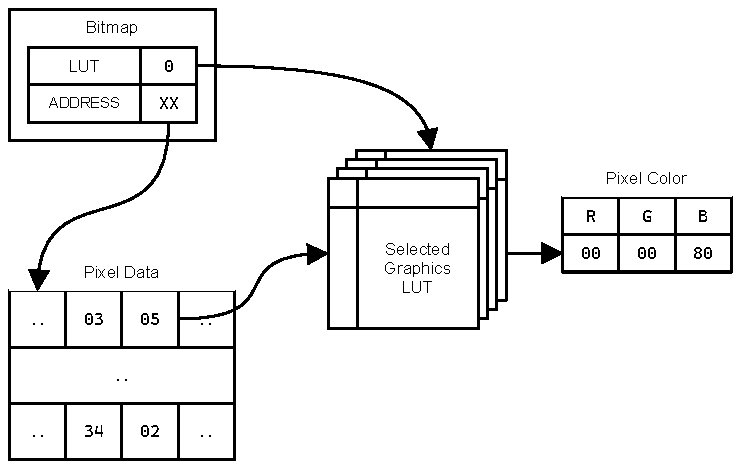
\includegraphics{images/bitmaps.pdf}
    \end{center}
    \caption{Bitmap Data to Pixels}
    \label{fig:bitmap_colors}
\end{figure}

However, there is a key difference from text mode. In text mode, there are two colors (foreground and background), and each color is one out of sixteen possibilities. With graphics modes, there are 256 possibilities. So a CLUT with only 16 entries will not work. There are therefore separate CLUTs for graphics. TinyVicky provides for four separate graphics CLUTs with 256 entries. Each graphic object on the screen specifies which graphics CLUT it will use for its colors. These CLUTs may be found in I/O page 0 (see table:~\ref{tab:graph_cluts}).

\begin{table}[ht]
    \begin{center}
        \begin{tabular}{|c|c|l|} \hline
            Address & R/W & Purpose \\\hline\hline
            \verb+0xD000+ & R/W & Graphics CLUT 0 \\ \hline
            \verb+0xD400+ & R/W & Graphics CLUT 1 \\ \hline
            \verb+0xD800+ & R/W & Graphics CLUT 2 \\ \hline
            \verb+0xDC00+ & R/W & Graphics CLUT 3 \\ \hline
        \end{tabular}
    \end{center}
    \caption{Graphics Color Lookup Tables}
    \label{tab:graph_cluts}
\end{table}

\example{A Simple Gradient}

Let's set up a CLUT so that we have the colors for a gradient fill between red and blue. In this example, \verb+pointer+ is a two byte variable down in zero page, which will be used to point to the first byte of the CLUT entry the code is updating. The \verb+Y+ register is being used to point to the individual components of the entry.

\begin{verbatim}
MMU_IO_CTRL = $0001             ; MMU I/O Control Register
VKY_GR_CLUT_0 = $D000           ; Graphics LUT #0

;
; Initialize the LUT to greyscale from (255, 0, 0) to (0, 0, 255)
;

            lda #$01            ; Set the I/O page to #1
            sta MMU_IO_CTRL

            lda #<VKY_GR_CLUT_0 ; pointer will be used to point to a particular LUT entry
            sta pointer
            lda #>VKY_GR_CLUT_0
            sta pointer+1

            ldx #0              ; Start with blue = 0

lut_loop:   ldy #0              ; And start at the offset for blue
            txa                 ; Take the current blue color level
            sta (pointer),y     ; Set the blue component
            iny

            lda #0
            sta (pointer),y     ; Set the green component to 0
            iny

            txa                 ; Get the blue component again
            eor #$ff            ; And compute the 2's complement of it
            inc a
            sta (pointer),y     ; Set the red component
            iny

            inx                 ; Go to the next color
            beq lut_done        ; If we are back to black, we're done with the LUT

            clc                 ; Move pointer to the next LUT entry (+ 4)
            lda pointer
            adc #4
            sta pointer
            lda pointer+1
            adc #0
            sta pointer+1

            bra lut_loop

lut_done:
\end{verbatim}

\section*{Pixel Data}

All three graphics engines arrange their pixel data in the same manner. They all use rectangular raster images as a base, although the width and height of the rectangle can vary. The pixels are placed in memory in sequential order in left-to-right and top-to-bottom order. That is, the first pixel in the sequence is the upper-left pixel in the image. The next pixel is the pixel to the immediate right and so on. If the image size is $w \times h$, the position of a pixel at $(x, y)$ in the list is $y \times w + x$.

\section*{Graphics Layers}

Now, what happens if two sprites take up the same position or if a program displays a tile map and a bitmap together? How does TinyVicky determine what color to display at a given position? TinyVicky provides a flexible layering system with several layers. Elements in ``near'' layers (lower numbers) get displayed on top of elements in ``far'' layers (higher numbers). If a sprite in layer 0 says a pixel should be blue while a tile in layer 1 says it should be red, the pixel will be blue. Color 0, however, is special. It is always the transparent ``color''. A pixel that is 0 in an element will be the color of whatever is behind it (or the global background color, if there is nothing behind it, see table~\ref{tab:back_reg}).

TinyVicky provides for seven layers, but they are split up a bit. Three of the layers are for bitmaps and tile maps. Only one bitmap or tile map can be placed in any of those three layers. The other four layers are for sprites only. Any sprite can be assigned to any of the sprite layers, and there can be multiple sprites in a layer. The sprite layers are interleaved with the bitmap and tile map layers (see figure:~\ref{fig:layers}).

\begin{figure}[ht]
    \begin{center}
        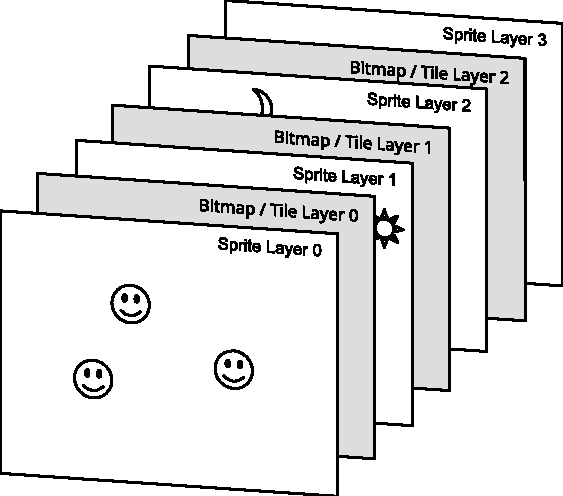
\includegraphics{images/Layers.pdf}
    \end{center}
    \caption{TinyVicky Graphic Layers}
    \label{fig:layers}
\end{figure}

Bitmaps and tile maps are assigned to their layers using the layer control registers (see table:~\ref{tab:bm_tm_layers}). The three fields LAYER0, LAYER1, and LAYER2 in the layer registers are three bit values, which indicate which graphical element to assign to that layer (see table:~\ref{tab:bm_tm_layer_codes}).

\begin{table}[ht]
    \begin{center}
        \begin{tabular}{|c|c|c|c|c|c|c|c|c|c|} \hline
            Address & R/W & 7 & 6 & 5 & 4 & 3 & 2 & 1 & 0 \\ \hline\hline
            \verb+0xD002+ & R/W & --- & \multicolumn{3}{|c|}{LAYER1} & --- & \multicolumn{3}{|c|}{LAYER0} \\\hline
            \verb+0xD003+ & R/W & \multicolumn{5}{|c|}{---} & \multicolumn{3}{|c|}{LAYER2} \\\hline
        \end{tabular}
    \end{center}
    \caption{Bitmap and Tile Map Layer Registers}
    \label{tab:bm_tm_layers}
\end{table}

\begin{table}[ht]
    \begin{center}
        \begin{tabular}{|c|l|} \hline
            Code & Layer \\ \hline\hline
            0 & Bitmap Layer 0 \\ \hline
            1 & Bitmap Layer 1 \\ \hline
            2 & Bitmap Layer 2 \\ \hline
            4 & Tile Map Layer 0 \\ \hline
            5 & Tile Map Layer 1 \\ \hline
            6 & Tile Map Layer 2 \\ \hline
        \end{tabular}
    \end{center}
    \caption{Bitmap and Tile Map Layer Codes}
    \label{tab:bm_tm_layer_codes}
\end{table}

\example{Put Bitmap 0 on Layer 0}

As an example of how to use layers, we can set things up for future examples by putting bitmap 0 in the front layer (0), tile map 0 in the next layer (1), and bitmap 1 in the back layer (2).

\begin{verbatim}
    lda #$40            ; Layer 0 = BM 0, Layer 1 = TM 0
    sta VKY_LAYER_CTRL_0
    lda #$01            ; Layer 2 = BM 1
    sta VKY_LAYER_CTRL_1
\end{verbatim}

\section{Bitmaps}

TinyVicky allows for three full screen bitmaps to be displayed at once. These bitmaps are either $320 \times 200$ or $320 \times 240$, depending on the value of the CLK\_70 bit of the master control register. A bitmap's pixel data contains either 64,000 bytes, or 76,800 bytes of data. In both cases, the pixel data is arranged from left to right and top to bottom. The first 320 bytes are the pixels of the first line (with the first pixel being the left-most). The second 320 bytes are the second line, and so on. Additionally, the bitmaps can independently use any of the four graphics CLUTs to specify the colors for those indexes. TinyVicky provides registers for each bitmap set the CLUT and the address of the bitmap:

\begin{table}[h]
    \begin{center}
        \begin{tabular}{|c|c|c|c|c|c|c|c|c|c|} \hline
            Address & Bitmap & 7 & 6 & 5 & 4 & 3 & 2 & 1 & 0 \\ \hline\hline
            \verb+0xD100+ & \multirow{4}{*}{0} & \multicolumn{5}{|c|}{---} & \multicolumn{2}{|c|}{CLUT} & ENABLE \\\cline{1-1}\cline{3-10}
            \verb+0xD101+ & & AD7 & AD6 & AD5 & AD4 & AD3 & AD2 & AD1 & AD0 \\\cline{1-1}\cline{3-10}
            \verb+0xD102+ & & AD15 & AD14 & AD13 & AD12 & AD11 & AD10 & AD9 & AD8 \\\cline{1-1}\cline{3-10}
            \verb+0xD103+ & & \multicolumn{6}{|c|}{---} & AD17 & AD16 \\ \hline
            
            \verb+0xD108+ & \multirow{4}{*}{1} & \multicolumn{5}{|c|}{---} & \multicolumn{2}{|c|}{CLUT} & ENABLE \\\cline{1-1}\cline{3-10}
            \verb+0xD109+ & & AD7 & AD6 & AD5 & AD4 & AD3 & AD2 & AD1 & AD0 \\\cline{1-1}\cline{3-10}
            \verb+0xD10A+ & & AD15 & AD14 & AD13 & AD12 & AD11 & AD10 & AD9 & AD8 \\\cline{1-1}\cline{3-10}
            \verb+0xD10B+ & & \multicolumn{6}{|c|}{---} & AD17 & AD16 \\ \hline

            \verb+0xD110+ & \multirow{4}{*}{2} & \multicolumn{5}{|c|}{---} & \multicolumn{2}{|c|}{CLUT} & ENABLE \\\cline{1-1}\cline{3-10}
            \verb+0xD111+ & & AD7 & AD6 & AD5 & AD4 & AD3 & AD2 & AD1 & AD0 \\\cline{1-1}\cline{3-10}
            \verb+0xD112+ & & AD15 & AD14 & AD13 & AD12 & AD11 & AD10 & AD9 & AD8 \\\cline{1-1}\cline{3-10}
            \verb+0xD113+ & & \multicolumn{6}{|c|}{---} & AD17 & AD16 \\ \hline
        \end{tabular}
    \end{center}
    \caption{Bitmap Registers}
    \label{tab:bm_registers}
\end{table}

\begin{description}
    \item[ENABLE] if set and both graphics and bitmaps are enabled in the Vicky Master Control Register (see table~\ref{tab:vky_master_ctrl_reg}), then this bitmap will be displayed.

    \item[CLUT] sets the graphics color lookup table to be used for this bitmap

    \item[AD] give the address of the first byte of the pixel data within the 256 KB system RAM. Note that this address is relative to the system bus of 20 bits and is not based on the CPU's addressing.
\end{description}

To set up and display a bitmap, the following things need to be done. The order is not terribly important, although updates to the bitmap's pixel data after the bitmap is displaying will be visible. That could be desirable, depending on what the program is doing.

\begin{enumerate}
    \item Enable bitmap graphics in the TinyVicky Master Control Register (see table:~\ref{tab:vky_master_ctrl_reg}). This means you need to set both the GRAPH and BITMAP bits and either clear TEXT or set the OVRLY to display text and bitmap together.

    \item Set up the pixel data for the bitmap somewhere in the first 256 KB of RAM.

    \item Set the address of the bitmap's pixel data in the AD field.

    \item Assign the bitmap to a layer using the layer control registers (see table:~\ref{tab:bm_tm_layers}).

    \item Set the bitmap's CLUT and ENABLE bit in its control register.
\end{enumerate}

\example{Display a Bitmap}

This example will build on the previous examples of setting up the CLUT and display a gradient on the screen. First, it needs to turn on the bitmap graphics:

\begin{verbatim}
            MMU_MEM_CTRL = $0000            ; MMU Memory Control Register
            MMU_IO_CTRL = $0001             ; MMU I/O Control Register
            VKY_MSTR_CTRL_0 = $D000         ; Vicky Master Control Register 0
            VKY_MSTR_CTRL_1 = $D001         ; Vicky Master Control Register 1
            VKY_BM0_CTRL = $D100            ; Bitmap #0 Control Register
            VKY_BM0_ADDR_L = $D101          ; Bitmap #0 Address bits 7..0
            VKY_BM0_ADDR_M = $D102          ; Bitmap #0 Address bits 15..8
            VKY_BM0_ADDR_H = $D103          ; Bitmap #0 Address bits 17..16

            bitmap_base = $10000            ; The base address of our bitmap

            stz MMU_IO_CTRL     ; Go back to I/O page #0

            lda #$0C            ; enable GRAPHICS and BITMAP. Disable TEXT
            sta VKY_MSTR_CTRL_0 ; Save that to VICKY master control register 0
            stz VKY_MSTR_CTRL_1 ; Make sure we're just in 320x240 mode (VICKY master control register 1)
\end{verbatim}

Next, it needs to set up the bitmap: setting the address, CLUT, and enabling the bitmap:

\begin{verbatim}
            ;
            ; Turn on bitmap #0
            ;

            stz VKY_BM1_CTRL    ; Make sure bitmap 1 is turned off

            lda #$01            ; Use graphics LUT #0, and enable bitmap
            sta VKY_BM0_CTRL

            lda #<bitmap_base   ; Set the low byte of the bitmap's address
            sta VKY_BM0_ADDR_L
            lda #>bitmap_base   ; Set the middle byte of the bitmap's address
            sta VKY_BM0_ADDR_M
            lda #`bitmap_base   ; Set the upper two bits of the bitmap's address
            and #$03
            sta VKY_BM0_ADDR_H
\end{verbatim}

Now, the code needs to create the pixel data for the gradient in memory. This is a bit tricky on the \jr, because the program is using the larger $320 \times 240$ screen, which requires more than 64 KB of memory. In order to write to the entire bitmap, the program will have to work with the MMU to switch memory banks to access the whole bitmap. The program will use bank 1 (0x2000 -- 0x3FFF) as its window into the bitmap, which will start at 0x10000. It will walk through the memory byte-by-byte, setting each pixel's color based on what line it is on (tracked in a \verb+line+ variable). Once it has written a bank's worth of pixels (8 KB), it will increment the bank number and update the MMU register. Once it has written 240 lines, it will finish.

NOTE: in the following code, \verb+bm_bank+ and \verb+line+ are byte variables, and \verb+pointer+ and \verb+column+ are two-byte variables in zero page (although really only \verb+pointer+ has to be there).

\begin{verbatim}
            ; Set the line number to 0
            stz line

            ; Calculate the bank number for the bitmap
            lda #(bitmap_base >> 13)
            sta bm_bank

bank_loop:  stz pointer         ; Set the pointer to start of the current bank
            lda #$20
            sta pointer+1

            ; Set the column to 0
            stz column
            stz column+1

            ; Alter the LUT entries for $2000 -> $bfff

            lda #$80            ; Turn on editing of MMU LUT #0, and work off #0
            sta MMU_MEM_CTRL

            lda bm_bank
            sta MMU_MEM_BANK_1  ; Set the bank we will map to $2000 - $3fff

            stz MMU_MEM_CTRL    ; Turn off editing of MMU LUT #0

            ; Fill the line with the color..

loop2:      lda line            ; The line number is the color of the line
            sta (pointer)

inc_column: inc column          ; Increment the column number
            bne chk_col
            inc column+1

chk_col:    lda column          ; Check to see if we have finished the row
            cmp #<320
            bne inc_point
            lda column+1
            cmp #>320
            bne inc_point

            lda line            ; If so, increment the line number
            inc a
            sta line
            cmp #240            ; If line = 240, we're done
            beq done

            stz column          ; Set the column to 0
            stz column+1

inc_point:  inc pointer         ; Increment pointer
            bne loop2           ; If < $4000, keep looping
            inc pointer+1
            lda pointer+1
            cmp #$40
            bne loop2

            inc bm_bank         ; Move to the next bank
            bra bank_loop       ; And start filling it

done:       nop                 ; Lock up here
            bra done
\end{verbatim}

\chapter{Sprites}

In addition to bitmaps and tiles, the \jr\ provides support for sprites, which are mobile graphical objects that can appear anywhere on the screen. \jr\ sprites are similar to the sprites on the Commodore 64 or player-missile graphics on the 8-bit Atari computers, but they are more flexible than either of those. A sprite is essentially a little bitmap that can be positioned anywhere on the screen. Each one can come in one of four sizes: $8 \times 8$, $16 \times 16$, $24 \times 24$, or $32 \times 32$. Each one can display up to 256 colors, picked from one of the four graphics color lookup tables.

A program for the \jr\ can use up to 64 sprites, each one of which is controlled by a block of sprite control registers. The sprite control registers are in I/O page 0, and start at 0xD900. Each sprite takes up 8 bytes, so sprite 0 starts at 0xD900, sprite 1 starts at 0xD908, sprite 2 at 0xD910, and so on. The registers for each sprite are arranged within that block of 8 bytes as shown in table~\ref{tab:sp_reg}.

\begin{table}[ht]
    \begin{center}
        \begin{tabular}{|c|c|c|c|c|c|c|c|c|c|} \hline
            Offset & R/W & 7 & 6 & 5 & 4 & 3 & 2 & 1 & 0 \\ \hline\hline
            0 & W & --- & \multicolumn{2}{|c|}{SIZE} & \multicolumn{2}{|c|}{LAYER} & \multicolumn{2}{|c|}{LUT} & ENABLE \\ \hline
            1 & W & AD7 & AD6 & AD5 & AD4 & AD3 & AD2 & AD1 & AD0 \\ \hline
            2 & W & AD15 & AD14 & AD13 & AD12 & AD11 & AD10 & AD9 & AD8 \\ \hline
            3 & W & \multicolumn{5}{|c|}{---} & AD18 & AD17 & AD16 \\ \hline
            4 & W & X7 & X6 & X5 & X4 & X3 & X2 & X1 & X0 \\ \hline
            5 & W & X15 & X14 & X13 & X12 & X11 & X10 & X9 & X8 \\ \hline
            6 & W & Y7 & Y6 & Y5 & Y4 & Y3 & Y2 & Y1 & Y0 \\ \hline
            7 & W & Y15 & Y14 & Y13 & Y12 & Y11 & Y10 & Y9 & Y8 \\ \hline
        \end{tabular}
    \end{center}
    \caption{Sprite Registers for a Single Sprite}
    \label{tab:sp_reg}
\end{table}

These registers manage seven fields:

\begin{description}
    \item[ENABLE] if set, this particular sprite will be displayed (assuming the graphics and sprite engines are enabled in the Vicky Master Control Register).

    \item[LUT] selects the graphics color lookup table to use in assigning colors to pixels

    \item[LAYER] selects which sprite layer the sprite will be displayed on

    \item[SIZE] selects the size of the sprite (see table~\ref{tab:sp_sizes})

    \item[AD] the address of the bitmap (must be within the first 512KB of RAM). The address is based on the 21-bit system bus, not the CPU's address space.

    \item[X] the X coordinate where the sprite will be displayed (corresponds to the sprite's upper-left corner)

    \item[Y] the Y coordinate where the sprite will be displayed (corresponds to the sprite's upper-left corner)
\end{description}

\begin{table}[ht]
    \begin{center}
        \begin{tabular}{|c|c|c|} \hline
            \multicolumn{2}{|c|}{SIZE} & Meaning \\ \hline\hline
            0 & 0 & $32 \times 32$ \\ \hline
            0 & 1 & $24 \times 24$ \\ \hline
            1 & 0 & $16 \times 16$ \\ \hline
            1 & 1 & $8 \times 8$ \\ \hline
        \end{tabular}
    \end{center}
    \caption{Sprite Sizes}
    \label{tab:sp_sizes}
\end{table}

\section*{Sprite, Layers, and Display Priority}

While a sprite can be assigned to any of four layers, this layer is only used for determining how the sprite interacts with bitmap or tile map graphics and not how sprites layer with each other. When sprites ``collide,'' a built-in sprite priority order is used to determine which sprite determines a pixel's color. When two sprites are both trying to set the color of a pixel on the screen, the sprite with the lowest number is the one that determines the color. For example, if sprite 0 and sprite 5 are in the same location, it is sprite 0 that will display in the foreground. The sprite layers {\em cannot} be used to change this.

The best practice for assigning sprites is to place the images that need to be on top in the first sprites and those that need to be in the back in the higher numbered sprites. Use the LAYER field for the sprites to control how the sprites layer with the tile maps and bitmaps.

\section*{Sprite Positioning}

The coordinate system for sprites is similar to that for bitmap graphics, but it is offset by 32 pixels in both the horizontal and vertical directions. There is a sort of margin area around the entire displayed screen that a sprite can be in and be either partially or completely hidden from view. The horizontal coordinate for a sprite ranges from 0 to 352. The vertical coordinate can range from 0 to 232 or 272, depending on the vertical resolution. For a sprite to have its top-left corner in the top-left of the screen, its position would need to be $(32, 32)$. This coordinate system is the same for all sprites, regardless of their size. Figure:~\ref{fig:sprite_positions} shows how the coordinate system is arranged.

\begin{figure}[ht]
    \begin{center}
        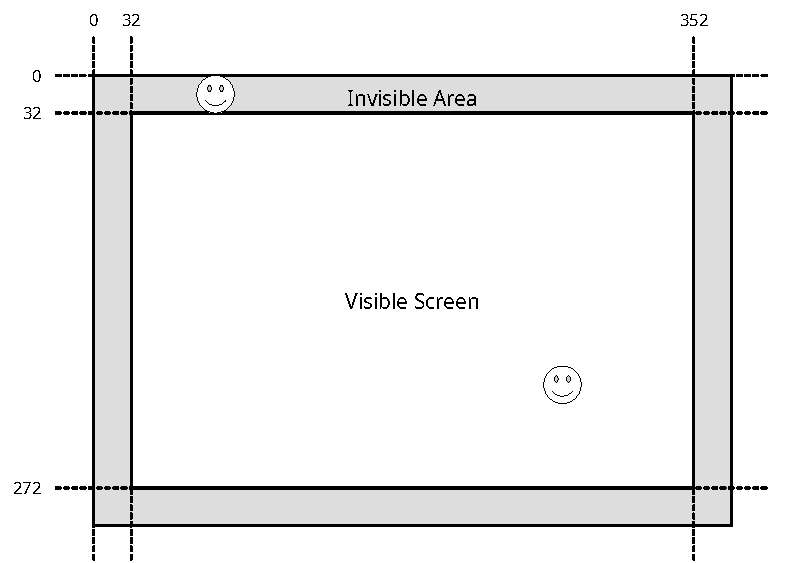
\includegraphics[scale=0.65]{images/SpritePositions.pdf}
    \end{center}
    \caption{Sprite Positions}
    \label{fig:sprite_positions}
\end{figure}

\example{Displaying a Sprite}
In this example, we'll just put a ball on the screen. First, the program needs to set up TinyVicky to be in sprite mode with no border and a light purple background:

\begin{verbatim}
MMU_IO_CTRL = $0001             ; MMU I/O Control Register

VKY_MSTR_CTRL_0 = $D000         ; Vicky Master Control Register 0
VKY_MSTR_CTRL_1 = $D001         ; Vicky Master Control Register 1
VKY_BRDR_CTRL = $D004           ; Vicky Border Control Register
VKY_BKG_COL_B = $D00D           ; Vicky Graphics Background Color Blue
VKY_BKG_COL_G = $D00E           ; Vicky Graphics Background Color Green
VKY_BKG_COL_R = $D00F           ; Vicky Graphics Background Color Red

VKY_SP0_CTRL = $D900            ; Sprite #0's control register
VKY_SP0_AD_L = $D901            ; Sprite #0's pixel data address register
VKY_SP0_AD_M = $D902
VKY_SP0_AD_H = $D903
VKY_SP0_POS_X_L = $D904         ; Sprite #0's X position register
VKY_SP0_POS_X_H = $D905
VKY_SP0_POS_Y_L = $D906         ; Sprite #0's Y position register
VKY_SP0_POS_Y_H = $D907

            ;
            ; Set up TinyVicky to display sprites
            ;
            lda #$24                    ; Graphics & Sprite engines enabled
            sta VKY_MSTR_CTRL_0
            stz VKY_MSTR_CTRL_1         ; 320x240 @ 60Hz

            stz VKY_BRDR_CTRL           ; No border

            lda #$96                    ; Background: lavender
            sta VKY_BKG_COL_R
            lda #$7B
            sta VKY_BKG_COL_G
            lda #$B6
            sta VKY_BKG_COL_B
\end{verbatim}

Next, the program loads the sprite's colors into the CLUT (\verb+ptr_src+ and \verb+ptr_dst+ are 16-bit storage locations in zero page and are used as pointers):

\begin{verbatim}
            ;
            ; Load the sprite LUT into memory
            ;

            lda #$01                    ; Switch to I/O Page #1
            sta MMU_IO_CTRL

            lda #<balls_clut_start      ; Set the source pointer to the palette
            sta ptr_src
            lda #>balls_clut_start
            sta ptr_src+1

            lda #<VKY_GR_CLUT_0         ; Set the destination to Graphics CLUT
            sta ptr_dst
            lda #>VKY_GR_CLUT_0
            sta ptr_dst+1

            ldx #0                      ; X is the number of colors copied
color_loop: ldy #0                      ; Y points to the color component
comp_loop:  lda (ptr_src),y             ; Read a byte from the code
            sta (ptr_dst),y             ; And write it to the CLUT
            iny                         ; Move to the next byte
            cpy #4
            bne comp_loop               ; Continue until 4 bytes copied

            inx                         ; Move to the next color
            cmp #16
            beq done_lut                ; Until we have copied all 16

            clc                         ; Move ptr_src to the next source color
            lda ptr_src
            adc #4
            sta ptr_src
            lda ptr_src+1
            adc #0
            sta ptr_src+1

            clc                         ; Move ptr_dst to the next destination
            lda ptr_dst
            adc #4
            sta ptr_dst
            lda ptr_dst+1
            adc #0
            sta ptr_dst+1

            bra color_loop              ; And start copying that new color

done_lut:   stz MMU_IO_CTRL             ; Go back to I/O Page 0
\end{verbatim}

Finally, we point sprite 0 to the pixel data (which is included in the assembly code below), set its location on the screen (which will be the upper left corner of the screen), and then we turn on the sprite setting its LUT and LAYER in the process:

\begin{verbatim}
            ;
            ; Set up sprite #0
            ;
init_sp0:   lda #<balls_img_start       ; Address = balls_img_start
            sta VKY_SP0_AD_L
            lda #>balls_img_start
            sta VKY_SP0_AD_M
            stz VKY_SP0_AD_H

            lda #32
            sta VKY_SP0_POS_X_L         ; (x, y) = (32, 32)... should be 
            stz VKY_SP0_POS_X_H         ; upper-left corner of the screen
            
            lda #32
            sta VKY_SP0_POS_Y_L
            stz VKY_SP0_POS_Y_H

            lda #$41                    ; Size=16x16, Layer=0, LUT=0, Enabled
            sta VKY_SP0_CTRL
\end{verbatim}

Here is the pixel data for the sprite:
\begin{verbatim}
balls_img_start:
.byte $0, $0, $0, $0, $0, $0, $3, $2, $2, $1, $0, $0, $0, $0, $0, $0
.byte $0, $0, $0, $0, $5, $5, $4, $3, $3, $3, $3, $2, $0, $0, $0, $0
.byte $0, $0, $0, $7, $7, $7, $6, $5, $4, $4, $3, $3, $1, $0, $0, $0
.byte $0, $0, $7, $9, $A, $B, $A, $8, $6, $5, $4, $3, $2, $1, $0, $0
.byte $0, $5, $7, $A, $D, $E, $D, $A, $7, $5, $5, $4, $3, $1, $1, $0
.byte $0, $5, $7, $B, $E, $E, $E, $C, $7, $5, $5, $4, $3, $1, $1, $0
.byte $3, $4, $6, $A, $D, $E, $D, $A, $7, $5, $5, $4, $3, $2, $1, $1
.byte $2, $3, $5, $8, $A, $C, $A, $8, $6, $5, $5, $4, $3, $2, $1, $1
.byte $2, $3, $4, $6, $7, $7, $7, $6, $5, $5, $5, $4, $3, $1, $1, $1
.byte $1, $3, $4, $5, $5, $5, $5, $5, $5, $5, $5, $3, $3, $1, $1, $1
.byte $0, $3, $3, $4, $5, $5, $5, $5, $5, $5, $4, $3, $2, $1, $1, $0
.byte $0, $2, $3, $3, $4, $4, $4, $4, $4, $3, $3, $2, $1, $1, $1, $0
.byte $0, $0, $1, $2, $3, $3, $3, $3, $3, $3, $2, $1, $1, $1, $0, $0
.byte $0, $0, $0, $1, $1, $1, $2, $2, $1, $1, $1, $1, $1, $0, $0, $0
.byte $0, $0, $0, $0, $1, $1, $1, $1, $1, $1, $1, $1, $0, $0, $0, $0
.byte $0, $0, $0, $0, $0, $0, $1, $1, $1, $1, $0, $0, $0, $0, $0, $0
\end{verbatim}

Here are the colors for the sprite (note that this example is using only 15 colors, to make the example more understandable in print):
\begin{verbatim}
balls_clut_start:
.byte $00, $00, $00, $00
.byte $88, $00, $00, $00
.byte $7C, $18, $00, $00
.byte $9C, $20, $1C, $00
.byte $90, $38, $1C, $00
.byte $B0, $40, $38, $00
.byte $A8, $54, $38, $00
.byte $C0, $5C, $50, $00
.byte $BC, $70, $50, $00
.byte $D0, $74, $68, $00
.byte $CC, $88, $68, $00
.byte $E0, $8C, $7C, $00
.byte $DC, $9C, $7C, $00
.byte $EC, $A4, $90, $00
.byte $EC, $B4, $90, $00
\end{verbatim}

\chapter{Tiles}
The third graphics engine TinyVicky provides is the tile map system. The tile map system might seem a bit confusing at first, but really it is very similar to text mode, just made more flexible. In text mode, we have characters (256 of them). The shapes of the characters are defined in the font. What character is shown in a particular spot on the screen is set in the text matrix, which is a rectangular array of bytes in memory. In the same way, with the tile system we have tiles (256 of those, too). What those tiles look like are defined in a ``tile set.'' What tile is shown in a particular spot on the screen is set in the ``tile map.'' So there is an analogy:

\begin{eqnarray*}
    {\rm character} & \approx & {\rm tile} \\
    {\rm font} & \approx & {\rm tile\ set} \\
    {\rm text\ matrix} & \approx & {\rm tile\ map} \\
\end{eqnarray*}

There are several differences with tile maps, however:

\begin{itemize}
    \item A tile map may use tiles that are either $8 \times 8$ pixels or $16 \times 16$ pixels.

    \item A tile map can be scrolled smoothly horizontally or vertically.

    \item A tile may use 256 colors in its pixels as opposed to text mode's two-color characters. This means that a tile set uses one byte per pixel, with that byte's value being an index into a CLUT (as with bitmaps and sprites), where text mode fonts are one {\em bit} per pixel choosing between a foreground and background color.

    \item The tile map system allows for up to eight different tile sets to be used at the same time, where text mode has a single font.

    \item Up to three different tile maps can be displayed at one time, where text mode can only display one text matrix.

    \item A tile map can be placed on any one of three display layers, where text mode is always on top.
\end{itemize}


\section*{Tile Maps}

There are three tile maps supported by TinyVicky, each of which has 13 bytes worth of registers (see table:~\ref{tab:tilemap_reg}). Tile map 0 starts at 0xD200. Tile map 1 starts at 0xD20C. Tile map 2 starts at 0xD218.

\begin{table}[ht]
    \begin{center}
        \begin{tabular}{|c|c|c|c|c|c|c|c|c|c|c|} \hline
            Offset & R/W & 7 & 6 & 5 & 4 & 3 & 2 & 1 & 0 \\ \hline\hline
            0 & W & \multicolumn{3}{|c|}{---} & TILE\_SIZE & \multicolumn{3}{|c|}{---} & ENABLE \\ \hline
            1 & W & AD7 & AD6 & AD5 & AD4 & AD3 & AD2 & AD1 & AD0 \\ \hline
            2 & W & AD15 & AD14 & AD13 & AD12 & AD11 & AD10 & AD9 & AD8 \\ \hline
            3 & W & \multicolumn{5}{|c|}{---} & AD18 & AD17 & AD16 \\ \hline
            4 & W & \multicolumn{8}{|c|}{MAP\_SIZE\_X} \\ \hline
            5 & W & \multicolumn{8}{|c|}{RESERVED} \\ \hline
            6 & W & \multicolumn{8}{|c|}{MAP\_SIZE\_Y} \\ \hline
            7 & W & \multicolumn{8}{|c|}{RESERVED} \\ \hline
            8 & W & X3 & X2 & X1 & X0 & SSX3 & SSX2 & SSX1 & SSX0 \\ \hline
            9 & W & DIR\_X & --- & X9 & X8 & X7 & X6 & X5 & X4 \\ \hline
            10 & W & Y3 & Y2 & Y1 & Y0 & SSY3 & SSY2 & SSY1 & SSY0 \\ \hline
            12 & W & DIR\_Y &\multicolumn{3}{|c|}{---} & Y7 & Y6 & Y5 & Y4 \\ \hline
        \end{tabular}
    \end{center}
    \caption{Tile Map Registers}
    \label{tab:tilemap_reg}
\end{table}

\begin{description}
    \item[TILE\_SIZE] if 0, tiles are 8 pixels wide by 8 tall. If 1, tiles are 16 pixels wide by 16 pixels tall

    \item[ENABLE] if set, the tile map will be displayed (if GRAPH and TILES are set in TinyVicky's Master Control Register)

    \item[AD] the address of the tile map data in RAM

    \item[MAP\_SIZE\_X] the width of the tile map in tiles ({\it i.e.} the number of columns)

    \item[MAP\_SIZE\_Y] the height of the tile map in tiles ({\it i.e.} the number of rows)

    \item[X] horizontal scroll in tile widths

    \item[SSX] horizontal scroll in pixels. How these bits are used varies with the size. If tiles are 16 pixels wide, then flags SSX[3..0] are used. If tiles are only 8 pixels wide, then only SSX[3..1] are used.

    \item[DIR\_X] the direction of the horizontal scroll.

    \item[Y] vertical scroll in tile heights

    \item[SSY] vertical scroll in pixels. How these bits are used varies with the size. If tiles are 16 pixels wide, then flags SSY[3..0] are used. If tiles are only 8 pixels wide, then only SSY[3..1] are used.

    \item[DIR\_Y] the direction of the vertical scroll.

\end{description}

One way tile maps get their flexibility is that, where text mode uses 8-bit bytes for the text matrix, a tile map is actually a rectangular collection of 16-bit integers in memory. A tile map entry is divided up into two pieces: the first byte is the number of the tile to display in that position (much like the character code in text mode), but the upper byte contains attribute bits (see table:~\ref{tab:tile_bits}), which have two fields:

\begin{description}
    \item[SET] is the number of the tile set to use for this tile's appearance

    \item[CLUT] is the number of the graphics CLUT to use in setting the colors
\end{description}

This attribute system makes tiles very powerful. Effectively, a single tile map can display 1,024 completely unique shapes at one time by using all eight tile sets. Also, since the CLUT is set for each tile in the attributes, the number of tiles needed can be reduced by clever use of recoloring.

\begin{table}[ht]
    \begin{center}
        \begin{tabular}{|c|c|c|c|c|c|c|c|c|c|c|c|c|c|c|c|} \hline
            15 & 14 & 13 & 12 & 11 & 10 & 9 & 8 & 7 & 6 & 5 & 4 & 3 & 2 & 1 & 0 \\ \hline\hline
            \multicolumn{3}{|c|}{---} & \multicolumn{2}{|c|}{CLUT} & \multicolumn{3}{|c|}{SET} & \multicolumn{8}{|c|}{TILE NUMBER} \\ \hline
        \end{tabular}
    \end{center}
    \caption{A Tile Map Entry}
    \label{tab:tile_bits}
\end{table}

\subsection*{Scrolling}

Tile maps can scroll across the screen both horizontally and vertically. The position of the tile map on the screen is controlled through the registers at offsets 8, 9, and 10. The horizontal position is controlled by DIR\_X, X, and SSX. The vertical position is controlled by DIR\_Y, Y, and SSY. The bits X and Y set the position in units of tiles. That is, the number in X[9..0] specifies how many complete tile columns the tile map is moved left or right. Likewise, Y[9..0] specifies how many tile rows the tile map is moved up or down. The SSX and SSY bits are used to specify how many rows of pixels within a tile the tile map is to move. SSX and SSY are therefore ``smooth scroll'' registers. They have a small trick to their use, however:

If the tile map uses tiles 16 pixels on a side, SSX[3..0] is used to specify the number of pixels to shift the tile map left or right: from 0 to 15. If, on the other hand, the tile map uses tiles 8 pixels on a side, only SSX[3..1] are used to specify the number of pixels to move: from 0 to 7. Note that SSX[0] is not used at all in this case. The SSY bits work in exactly the same way for smooth scrolling in the vertical direction.

Finally, DIR\_X and DIR\_Y are used to control the direction of the scrolling. If DIR\_X is 0, the tile map will move to the left. If DIR\_X is 1, the tile map will move to the right. If DIR\_Y is 0, the tile map will move to up. If DIR\_Y is 1, the tile map will move down. Note that the representation of the amount of the scrolling is separate from the direction (set X to 3 to scroll by 3 tiles, whether that is 3 to the left or 3 to the right). One way to look at the scroll registers is that they are one's complement numbers: a magnitude and a separate sign bit.

To make sure that scrolling will work properly, the tile map needs to be at least as big as the full screen (even if it is largely ``empty''), and there should be blank columns to the left and the right and blank rows above and below. That is, it is best to leave an empty margin all the way around your working tile map.

\section*{Tile Sets}

Essentially, a tile set is just a bitmap, but of a smaller size and arranged in a specific pattern. A tile set can be either a linear arrangement of tiles or a square arrangement of tiles. In the linear arrangement, the image is one tile wide by 256 tiles high. So for $8 \times 8$ tiles, the tile set is 8 pixels wide by 2,048 pixels high. For $16 \times 16$ tiles, the tile set is 16 pixels wide by 4,096 pixels high. The tiles are arranged vertically, so the first 8 or 16 (depending on tile size) rows are tile 0, the second set of rows are tile 1, and so on. For the square arrangement, the tile set is either 128 pixels wide by 128 pixels high (for $8 \times 8$ tiles), or it is 256 pixels wide by 256 pixels high (for $16 \times 16$ tiles). In both cases, the tiles are laid out left to right and top to bottom in a grid that is 16 tiles wide by 16 tiles high (see table~\ref{tab:tile_set_layout}).

As with bitmaps and sprites, the pixels of the tiles are each an individual byte. The contents of the byte (0 -- 255) serving as an index into a color lookup table. The pixels are also laid out in left-to-right and top-to-bottom order, just as with bitmaps and individual sprites.

\begin{table}[ht]
    \begin{center}
        \begin{tabular}{|c|c|c|c|c|c|c|c|c|c|c|c|c|c|c|c|c|} \hline
            & \multicolumn{16}{|c|}{128 or 256 pixels} \\ \hline
            \multirow{16}{*}{\rotatebox{90}{128 or 256 pixels}}
            & 0 & 1 & 2 & 3 & 4 & 5 & 6 & 7 & 8 & 9 & 10 & 11 & 12 & 13 & 14 & 15 \\ \cline{2-17}
            & 16 & 17 & 18 & 19 & 20 & 21 & 22 & 23 & 24 & 25 & 26 & 27 & 28 & 29 & 30 & 31 \\ \cline{2-17}
            & 32 & 33 & 34 & 35 & 36 & 37 & 38 & 39 & 40 & 41 & 42 & 43 & 44 & 45 & 46 & 46 \\ \cline{2-17}
            & 48 & 49 & 50 & 51 & 52 & 53 & 54 & 55 & 56 & 57 & 58 & 59 & 60 & 61 & 62 & 63 \\ \cline{2-17}
            & 64 & 65 & 66 & 67 & 68 & 69 & 60 & 71 & 72 & 73 & 74 & 75 & 76 & 77 & 78 & 79 \\ \cline{2-17}
            & 80 & 81 & 82 & 83 & 84 & 85 & 86 & 87 & 88 & 89 & 90 & 91 & 92 & 93 & 94 & 95 \\ \cline{2-17}
            & 96 & 97 & 98 & 99 & 100 & 101 & 102 & 103 & 104 & 105 & 106 & 107 & 108 & 109 & 110 & 111 \\ \cline{2-17}
            & 112 & 113 & 114 & 115 & 116 & 117 & 118 & 119 & 120 & 121 & 122 & 123 & 124 & 125 & 126 & 127 \\ \cline{2-17}
            & 128 & 129 & 130 & 131 & 132 & 133 & 134 & 135 & 136 & 137 & 138 & 139 & 140 & 141 & 142 & 143 \\ \cline{2-17}
            & 144 & 145 & 146 & 147 & 148 & 149 & 150 & 151 & 152 & 153 & 154 & 155 & 156 & 157 & 158 & 159 \\ \cline{2-17}
            & 160 & 161 & 162 & 163 & 164 & 165 & 166 & 167 & 168 & 169 & 170 & 171 & 172 & 173 & 174 & 175 \\ \cline{2-17}
            & 176 & 177 & 178 & 179 & 180 & 181 & 182 & 183 & 184 & 185 & 186 & 187 & 188 & 189 & 190 & 191 \\ \cline{2-17}
            & 192 & 193 & 194 & 195 & 196 & 197 & 198 & 199 & 200 & 201 & 202 & 203 & 204 & 205 & 206 & 207 \\ \cline{2-17}
            & 208 & 209 & 210 & 211 & 212 & 213 & 214 & 215 & 216 & 217 & 218 & 219 & 220 & 221 & 222 & 223 \\ \cline{2-17}
            & 224 & 225 & 226 & 227 & 228 & 229 & 230 & 231 & 232 & 233 & 234 & 235 & 236 & 237 & 238 & 239 \\ \cline{2-17}
            & 240 & 241 & 242 & 243 & 244 & 245 & 246 & 247 & 248 & 249 & 250 & 251 & 252 & 253 & 254 & 255 \\ \hline
        \end{tabular}
    \end{center}
    \caption{Arrangement of Tiles in a Tile Set Image}
    \label{tab:tile_set_layout}
\end{table}

TinyVicky supports eight separate tile sets. Each one has a single three byte address register, which provides the address to the tile set pixel data, and a configuration register (see table:~\ref{tab:tile_set_addr}). To use them, a program simply stores the address of the pixel data to use into the appropriate address register. The configuration register contains a single SQUARE flag, which indicates the layout of the tile set image. If SQUARE is set (1), the tile set image is square ($128 \times 128$ pixels for $8 \times 8$ tiles or $256 \times 256$ pixels for $16 \times 16$ tiles). If SQUARE is clear (0), the tile set image is vertical ($8 \times 2,048$ pixels for $8 \times 8$ tiles, or $16 \times 4,096$ pixels for $16 \times 16$ tiles).

\begin{table}[ht]
    \begin{center}
        \begin{tabular}{|c|c|c|c|c|c|c|c|c|c|c|} \hline
            Address & R/W & Tile Set & 7 & 6 & 5 & 4 & 3 & 2 & 1 & 0 \\ \hline\hline
            \verb+0xD280+ & W & \multirow{4}{*}{0} & AD7 & AD6 & AD5 & AD4 & AD3 & AD2 & AD1 & AD0 \\ \cline{1-2}\cline{4-11}
            \verb+0xD281+ & W &                    & AD15 & AD14 & AD13 & AD12 & AD11 & AD10 & AD9 & AD8 \\ \cline{1-2}\cline{4-11}
            \verb+0xD282+ & W &                    & \multicolumn{5}{|c|}{---} & AD18 & AD17 & AD16 \\ \cline{1-2}\cline{4-11}
            \verb+0xD283+ & W &                    & \multicolumn{4}{|c|}{---} & SQUARE & \multicolumn{3}{|c|}{---} \\ \hline\hline

            \verb+0xD284+ & W & \multirow{4}{*}{1} & AD7 & AD6 & AD5 & AD4 & AD3 & AD2 & AD1 & AD0 \\ \cline{1-2}\cline{4-11}
            \verb+0xD285+ & W &                    & AD15 & AD14 & AD13 & AD12 & AD11 & AD10 & AD9 & AD8 \\ \cline{1-2}\cline{4-11}
            \verb+0xD286+ & W &                    & \multicolumn{5}{|c|}{---} & AD18 & AD17 & AD16 \\ \cline{1-2}\cline{4-11}
            \verb+0xD287+ & W &                    & \multicolumn{4}{|c|}{---} & SQUARE & \multicolumn{3}{|c|}{---} \\ \hline\hline

            \verb+0xD288+ & W & \multirow{4}{*}{2} & AD7 & AD6 & AD5 & AD4 & AD3 & AD2 & AD1 & AD0 \\ \cline{1-2}\cline{4-11}
            \verb+0xD289+ & W &                    & AD15 & AD14 & AD13 & AD12 & AD11 & AD10 & AD9 & AD8 \\ \cline{1-2}\cline{4-11}
            \verb+0xD28A+ & W &                    & \multicolumn{5}{|c|}{---} & AD18 & AD17 & AD16 \\ \cline{1-2}\cline{4-11}
            \verb+0xD28B+ & W &                    & \multicolumn{4}{|c|}{---} & SQUARE & \multicolumn{3}{|c|}{---} \\ \hline\hline

            \verb+0xD28C+ & W & \multirow{4}{*}{3} & AD7 & AD6 & AD5 & AD4 & AD3 & AD2 & AD1 & AD0 \\ \cline{1-2}\cline{4-11}
            \verb+0xD28D+ & W &                    & AD15 & AD14 & AD13 & AD12 & AD11 & AD10 & AD9 & AD8 \\ \cline{1-2}\cline{4-11}
            \verb+0xD28E+ & W &                    & \multicolumn{5}{|c|}{---} & AD18 & AD17 & AD16 \\ \cline{1-2}\cline{4-11}
            \verb+0xD28F+ & W &                    & \multicolumn{4}{|c|}{---} & SQUARE & \multicolumn{3}{|c|}{---} \\ \hline\hline
        \end{tabular}
    \end{center}
    \caption{Tile Set 0--3 Registers}
    \label{tab:tile_set_addr}
\end{table}

\begin{table}[ht]
    \begin{center}
        \begin{tabular}{|c|c|c|c|c|c|c|c|c|c|c|} \hline
            Address & R/W & Tile Set & 7 & 6 & 5 & 4 & 3 & 2 & 1 & 0 \\ \hline\hline
            \verb+0xD290+ & W & \multirow{4}{*}{4} & AD7 & AD6 & AD5 & AD4 & AD3 & AD2 & AD1 & AD0 \\ \cline{1-2}\cline{4-11}
            \verb+0xD291+ & W &                    & AD15 & AD14 & AD13 & AD12 & AD11 & AD10 & AD9 & AD8 \\ \cline{1-2}\cline{4-11}
            \verb+0xD292+ & W &                    & \multicolumn{5}{|c|}{---} & AD18 & AD17 & AD16 \\ \cline{1-2}\cline{4-11}
            \verb+0xD293+ & W &                    & \multicolumn{4}{|c|}{---} & SQUARE & \multicolumn{3}{|c|}{---} \\ \hline\hline

            \verb+0xD294+ & W & \multirow{4}{*}{5} & AD7 & AD6 & AD5 & AD4 & AD3 & AD2 & AD1 & AD0 \\ \cline{1-2}\cline{4-11}
            \verb+0xD295+ & W &                    & AD15 & AD14 & AD13 & AD12 & AD11 & AD10 & AD9 & AD8 \\ \cline{1-2}\cline{4-11}
            \verb+0xD296+ & W &                    & \multicolumn{5}{|c|}{---} & AD18 & AD17 & AD16 \\ \cline{1-2}\cline{4-11}
            \verb+0xD297+ & W &                    & \multicolumn{4}{|c|}{---} & SQUARE & \multicolumn{3}{|c|}{---} \\ \hline\hline

            \verb+0xD298+ & W & \multirow{4}{*}{6} & AD7 & AD6 & AD5 & AD4 & AD3 & AD2 & AD1 & AD0 \\ \cline{1-2}\cline{4-11}
            \verb+0xD299+ & W &                    & AD15 & AD14 & AD13 & AD12 & AD11 & AD10 & AD9 & AD8 \\ \cline{1-2}\cline{4-11}
            \verb+0xD29A+ & W &                    & \multicolumn{5}{|c|}{---} & AD18 & AD17 & AD16 \\ \cline{1-2}\cline{4-11}
            \verb+0xD29B+ & W &                    & \multicolumn{4}{|c|}{---} & SQUARE & \multicolumn{3}{|c|}{---} \\ \hline\hline

            \verb+0xD29C+ & W & \multirow{4}{*}{7} & AD7 & AD6 & AD5 & AD4 & AD3 & AD2 & AD1 & AD0 \\ \cline{1-2}\cline{4-11}
            \verb+0xD29D+ & W &                    & AD15 & AD14 & AD13 & AD12 & AD11 & AD10 & AD9 & AD8 \\ \cline{1-2}\cline{4-11}
            \verb+0xD29E+ & W &                    & \multicolumn{5}{|c|}{---} & AD18 & AD17 & AD16 \\ \cline{1-2}\cline{4-11}
            \verb+0xD29F+ & W &                    & \multicolumn{4}{|c|}{---} & SQUARE & \multicolumn{3}{|c|}{---} \\ \hline
        \end{tabular}
    \end{center}
    \caption{Tile Set Registers 4--7}
    \label{tab:tile_set_addr_4_7}
\end{table}

\example{A Simple Tile Map}

\begin{verbatim}
            ;
            ; Set up TinyVicky to display tiles
            ;
            lda #$14                    ; Graphics and Tile engines enabled
            sta VKY_MSTR_CTRL_0
            stz VKY_MSTR_CTRL_1         ; 320x240 @ 60Hz

            lda #$40                    ; Layer 0 = Bitmap 0, Layer 1 = Tile map 0
            sta VKY_LAYER_CTRL_0
            lda #$15                    ; Layer 2 = Tile Map 1
            sta VKY_LAYER_CTRL_1

            stz VKY_BRDR_CTRL           ; No border

            lda #$19                    ; Background: midnight blue
            sta VKY_BKG_COL_R
            lda #$19
            sta VKY_BKG_COL_G
            lda #$70
            sta VKY_BKG_COL_B
\end{verbatim}

To define the tile set, all we really need to do is to set the address register for the tile set to point to the actual pixel data. In this particular case, the code is just going to use tile set 0.

\begin{verbatim}
            ;
            ; Set tile set #0 to our image
            ;

            lda #<tiles_img_start
            sta VKY_TS0_ADDR_L
            lda #>tiles_img_start
            sta VKY_TS0_ADDR_M
            lda #`tiles_img_start
            sta VKY_TS0_ADDR_H
\end{verbatim}

Finally, the code sets up the tile map itself, setting the size of the tiles, the size of the tile map, setting the position of the screen in the tile map, and pointing to the tile map data.

\begin{verbatim}
            ;
            ; Set tile map #0
            ;

            lda #$01                    ; 16x16 tiles, enable
            sta VKY_TM0_CTRL

            lda #22                     ; Our tile map is 20x15
            sta VKY_TM0_SIZE_X
            lda #16
            sta VKY_TM0_SIZE_Y

            lda #<tile_map              ; Point to the tile map
            sta VKY_TM0_ADDR_L
            lda #>tile_map
            sta VKY_TM0_ADDR_M
            lda #`tile_map
            sta VKY_TM0_ADDR_H

            lda #$0F                    ; Set scrolling (15, 0)
            sta VKY_TM0_POS_X_L
            lda #$00
            sta VKY_TM0_POS_X_H

            stz VKY_TM0_POS_Y_L
            stz VKY_TM0_POS_Y_H
\end{verbatim}

The tile map itself. In this case, we just define it in-line. The data is formatted to match the dimensions of the tile map for ease of reading. Note that the left-most and right-most columns are essentially blank, providing some buffer space to allow for scrolling. Similarly, there is a spare row on the bottom. This data is formatted as single hexadecimal digits, to make it easier to format this data on the page, but the data is actually stored as 16-bit values. This is taking advantage of the fact that the code is using CLUT 0 and LAYER 0 for the tiles and that there are no more than 16 tiles in the tile set.

\begin{verbatim}
tile_map:
.word $4,$1,$0,$1,$0,$0,$0,$0,$0,$0,$0,$0,$0,$0,$0,$0,$0,$0,$4,$0,$4,$0
.word $0,$0,$1,$0,$0,$0,$0,$0,$0,$0,$0,$0,$0,$0,$0,$0,$0,$0,$0,$4,$0,$0
.word $0,$1,$0,$1,$0,$0,$6,$7,$7,$7,$7,$7,$7,$7,$7,$8,$0,$0,$4,$0,$4,$0
.word $0,$0,$0,$0,$0,$0,$9,$1,$2,$3,$4,$5,$0,$0,$0,$A,$0,$0,$0,$0,$0,$0
.word $0,$0,$0,$0,$0,$0,$9,$2,$1,$2,$3,$4,$5,$0,$0,$A,$0,$0,$0,$0,$0,$0
.word $0,$0,$0,$0,$0,$0,$9,$3,$2,$1,$2,$3,$4,$5,$0,$A,$0,$0,$0,$0,$0,$0
.word $0,$0,$0,$0,$0,$0,$9,$4,$3,$2,$1,$2,$3,$4,$5,$A,$0,$0,$0,$0,$0,$0
.word $0,$0,$0,$0,$0,$0,$9,$5,$4,$3,$2,$1,$2,$3,$4,$A,$0,$0,$0,$0,$0,$0
.word $0,$0,$0,$0,$0,$0,$9,$0,$5,$4,$3,$2,$1,$2,$3,$A,$0,$0,$0,$0,$0,$0
.word $0,$0,$0,$0,$0,$0,$9,$0,$0,$5,$4,$3,$2,$1,$2,$A,$0,$0,$0,$0,$0,$0
.word $0,$0,$0,$0,$0,$0,$9,$0,$0,$0,$5,$4,$3,$2,$1,$A,$0,$0,$0,$0,$0,$0
.word $0,$0,$0,$0,$0,$0,$B,$C,$C,$C,$C,$C,$C,$C,$C,$D,$0,$0,$0,$0,$0,$0
.word $0,$3,$0,$3,$0,$0,$0,$0,$0,$0,$0,$0,$0,$0,$0,$0,$0,$0,$2,$0,$2,$0
.word $0,$0,$3,$0,$0,$0,$0,$0,$0,$0,$0,$0,$0,$0,$0,$0,$0,$0,$0,$2,$0,$0
.word $0,$3,$0,$3,$0,$0,$0,$0,$0,$0,$0,$0,$0,$0,$0,$0,$0,$0,$2,$0,$2,$0
.word $0,$0,$0,$0,$0,$0,$0,$0,$0,$0,$0,$0,$0,$0,$0,$0,$0,$0,$2,$0,$0,$4
\end{verbatim}

\chapter{Miscellaneous Features of TinyVicky}

\section*{DIP Switches}

\jr\ has eight DIP switches on the board, which can be used to configure various options. The DIP switches are present on a single register (see table:~\ref{tab:dip_reg}). The DIP switches ground their signals when placed in their ``on'' positions. So a true or asserted value is 0, while the false or de-asserted value is 1.

\begin{table}[ht]
    \begin{center}
        \begin{tabular}{|c|c|c|c|c|c|c|c|c|c|} \hline
            Address & R/W & 7 & 6 & 5 & 4 & 3 & 2 & 1 & 0 \\\hline\hline
            \verb+0xD670+ & R & GAMMA & USER2 & USER1 & USER0 & \multicolumn{4}{|c|}{BOOT} \\ \hline
        \end{tabular}
    \end{center}
    \caption{DIP Switch Register}
    \label{tab:dip_reg}
\end{table}

There are five fields of switches:
\begin{description}
    \item[GAMMA] this is a dedicated switch to indicate if gamma correction should be turned on (0) or not (1)

    \item[USER0, USER1, USER2] these three switches are reserved for use by the operating system or programs. On is 0, off is 1.

    \item[BOOT] these four switches provide information to the operating system for boot options.
\end{description}

\section*{The Border}

The \jr's display can have a border, which overlays all the other display elements. The border can have any color which TinyVicky can display, and can have a width from 0 to 31 pixels. The border can also be turned off, leaving the full display for graphics or text.

When using graphics modes, the border simply hides the graphics elements underneath it. For text mode, things are a little different. The text display will be shifted so that the character at $(0, 0)$ is still the upper-left character. The layout of the text and color matrixes do not change, however. Cells that are under the right side or bottom of the border will still be in the matrixes but will not be displayed. Another way to put it is that, if the text resolution is 80 characters wide, it will remain 80 characters per line even if the border is on and only 76 characters are displayed.

\begin{table}[ht]
    \begin{center}
        \begin{tabular}{|c|c|c|c|c|c|c|c|c|c|c|} \hline
            Address & R/W & Name & 7 & 6 & 5 & 4 & 3 & 2 & 1 & 0 \\\hline\hline
            \verb+0xD004+ & R/W & BRDR\_CTRL & --- & \multicolumn{3}{|c|}{SCROLL\_X} & \multicolumn{3}{|c|}{---} & ENABLE \\ \hline
            \verb+0xD005+ & R/W & BRDR\_BLUE & \multicolumn{8}{|c|}{Blue component of border color} \\ \hline
            \verb+0xD006+ & R/W & BRDR\_GREEN & \multicolumn{8}{|c|}{Green component of border color} \\ \hline
            \verb+0xD007+ & R/W & BRDR\_RED & \multicolumn{8}{|c|}{Red component of border color} \\ \hline
            \verb+0xD008+ & R/W & BRDR\_WIDTH & \multicolumn{3}{|c|}{---} & \multicolumn{5}{|c|}{SIZE\_X} \\ \hline
            \verb+0xD009+ & R/W & BRDR\_HEIGHT & \multicolumn{3}{|c|}{---} & \multicolumn{5}{|c|}{SIZE\_Y} \\ \hline
        \end{tabular}
    \end{center}
    \caption{Border Registers}
    \label{tab:brdr_reg}
\end{table}

\begin{description}
    \item[ENABLE] when set (1), the border will be displayed

    \item[SCROLL\_X] the number of pixels the border should be shifted in the horizontal direction

    \item[BRDR\_BLUE] the amount of blue in the border (0 = none, 255 = maximum amount)

    \item[BRDR\_GREEN] the amount of green in the border (0 = none, 255 = maximum amount)

    \item[BRDR\_RED] the amount of red in the border (0 = none, 255 = maximum amount)

    \item[SIZE\_X] the width of the left and right sides of the border in pixels (from 0 to 31)

    \item[SIZE\_Y] the height of top and bottom of the border in pixels (from 0 to 31)
\end{description}

\section*{Background Color}

In text mode, the background color is determined by the color matrix and the text color LUTs. For the graphics modes, however, a background color is specified separately. There are three registers to specify the background color's red, green, and blue components (see table:~\ref{tab:back_reg}). This is the color that will be displayed in graphics modes, if all the layers specify that a given pixel has the color 0 (which is always the transparent pixel color).

\begin{table}[ht]
    \begin{center}
        \begin{tabular}{|c|c|c|c|c|c|c|c|c|c|c|} \hline
            Address & R/W & Name & 7 & 6 & 5 & 4 & 3 & 2 & 1 & 0 \\\hline\hline
            \verb+0xD00D+ & R/W & BGND\_BLUE & \multicolumn{8}{|c|}{Blue component of background color} \\ \hline
            \verb+0xD00E+ & R/W & BGND\_GREEN & \multicolumn{8}{|c|}{Green component of background color} \\ \hline
            \verb+0xD00F+ & R/W & BGND\_RED & \multicolumn{8}{|c|}{Red component of background color} \\ \hline
        \end{tabular}
    \end{center}
    \caption{Background Color Registers}
    \label{tab:back_reg}
\end{table}

\section*{Line Interrupt and Beam Position}

TinyVicky can trigger a SOL interrupt (see table:~\ref{tab:int_group_0}) when the display has reached a given raster line. This can be useful for split-screen style effects or other programming tricks that work off of partitioning the screen into separate areas. To use this feature, a program would enable the line interrupt and set a register to the number of the line on the screen when the interrupt should be triggered. In addition to setting a line interrupt, there are two 12-bit registers that allow the program to see what line and column is TinyVicky is currently drawing. The addresses for all these registers overlap. The line interrupt registers are write-only, and the current beam position registers are read only (see table:~\ref{tab:lint_reg})

\begin{table}[ht]
    \begin{center}
        \begin{tabular}{|c|c|c|c|c|c|c|c|c|c|c|} \hline
            Address & R/W & Name & 7 & 6 & 5 & 4 & 3 & 2 & 1 & 0 \\\hline\hline
            \verb+0xD018+ & W & LINT\_CTRL & \multicolumn{7}{|c|}{---} & ENABLE \\ \hline
            \verb+0xD019+ & W & \multirow{2}{*}{LINT\_L} & L7 & L6 & L5 & L4 & L3 & L2 & L1 & L0 \\ \cline{1-2}\cline{4-11}
            \verb+0xD01A+ & W &  & \multicolumn{4}{|c|}{---} & L11 & L10 & L9 & L8 \\ \hline
            \verb+0xD01B+ & W & --- & \multicolumn{8}{|c|}{Reserved} \\ \hline

            \verb+0xD018+ & R & \multirow{2}{*}{RAST\_COL} & X7 & X6 & X5 & X4 & X3 & X2 & X1 & X0 \\  \cline{1-2}\cline{4-11}
            \verb+0xD019+ & R & & \multicolumn{4}{|c|}{---} & X11 & X10 & X9 & X8 \\ \hline
            \verb+0xD01A+ & R & \multirow{2}{*}{RAST\_ROW} & Y7 & Y6 & Y5 & Y4 & Y3 & Y2 & Y1 & Y0 \\  \cline{1-2}\cline{4-11}
            \verb+0xD01B+ & R & & \multicolumn{4}{|c|}{---} & Y11 & Y10 & Y9 & Y8 \\ \hline
        \end{tabular}
    \end{center}
    \caption{Line Interrupt and Beam Position Registers}
    \label{tab:lint_reg}
\end{table}

\begin{description}
    \item[ENABLE] if set (1), TinyVicky will trigger line interrupts (write only)

    \item[LINT\_L] the line number (12 bits) on which to trigger the next line interrupt (write only). The top of the display is line 0, and the bottom of the screen is 400 for $320 \times 200$ mode, and 480 for $320 \times 240$ mode.

    \item[RAST\_COL] the number (12 bits) of the current pixel being drawn (read only)

    \item[RAST\_ROW] the number (12 bits) of the current line being drawn (read only)
\end{description}

\example{Changing Border with the Line}
In this example, we will play with a split-screen style effect changing the color of the border so that the top and bottom borders are blue while the left and right borders are red. To do this, we will use the line interrupt twice for each frame: once when we are on the line just below the last line of the top border, and once when we are on the first line of the bottom border.

To make this work, the example has a single \verb+state+ variable, which will track which color border is being rendered. It will enable the line interrupt, and then set the line number to wait for. When that interrupt comes in, it will check the state variable, setting the border color and new line number based on \verb+state+. It will also flip \verb+state+ to the other value (0 or 1).

\begin{verbatim}
INT_PEND_0 = $D660              ; Pending register for interrupts 0 - 7
INT_PEND_1 = $D661              ; Pending register for interrupts 8 - 15
INT_MASK_0 = $D666              ; Mask register for interrupts 0 - 7
INT_MASK_1 = $D667              ; Mask register for interrupts 8 - 15
INT01_VKY_SOL = $02

MMU_IO_CTRL = $0001             ; MMU I/O Control Register

VKY_MSTR_CTRL_0 = $D000         ; Vicky Master Control Register 0
VKY_MSTR_CTRL_1 = $D001         ; Vicky Master Control Register 1
VKY_BRDR_CTRL = $D004           ; Vicky Border Control Register
VKY_BRDR_COL_B = $D005          ; Vicky Border Color -- Blue
VKY_BRDR_COL_G = $D006          ; Vicky Border Color -- Green
VKY_BRDR_COL_R = $D007          ; Vicky Border Color -- Red
VKY_BRDR_VERT = $D008           ; Vicky Border vertical thickness in pixels
VKY_BRDR_HORI = $D009           ; Vicky Border Horizontal Thickness in pixels

VIRQ = $FFFE

LINE0 = 16                      ; Start at line 16 (first line on the text display)
LINE1 = 480 - 16                ; End on line 464 (last line of text display)

;
; Variables
;
* = $0080

state       .byte ?             ; Variable to track which color we should use

;
; Code
;
* = $e000

start:      ; Disable IRQ handling
            sei

            ; Go back to I/O page 0
            stz MMU_IO_CTRL

            ; Load my IRQ handler into the IRQ vector
            ; NOTE: this code just takes over IRQs completely. It could save
            ;       the pointer to the old handler and chain to it when it had
            ;       handled its interrupt. But what is proper really depends on
            ;       what the program is trying to do.
            lda #<my_handler
            sta VIRQ
            lda #>my_handler
            sta VIRQ+1

            ; Mask off all but the SOL interrupt
            lda #$ff
            sta INT_MASK_1
            and #~INT01_VKY_SOL
            sta INT_MASK_0

            ; Clear all pending interrupts
            lda #$ff
            sta INT_PEND_0
            sta INT_PEND_1

            ; Make sure we're in text mode
            lda #$01                ; enable TEXT
            sta VKY_MSTR_CTRL_0     ; Save to VICKY master control register 0
            stz VKY_MSTR_CTRL_1

            ; Set the border
            lda #$01                ; Enable the border
            sta VKY_BRDR_CTRL

            lda #16                 ; Make it 16 pixels wide
            sta VKY_BRDR_VERT
            sta VKY_BRDR_HORI

            lda #$80                ; Make it cyan to start with
            sta VKY_BRDR_COL_B
            sta VKY_BRDR_COL_G
            stz VKY_BRDR_COL_R

            lda #$01                ; Turn on the line interrupt
            sta VKY_LINE_CTRL

            lda #<LINE0             ; set the line to interrupt on
            sta VKY_LINE_NBR_L
            lda #>LINE0
            sta VKY_LINE_NBR_H

            stz state               ; Start in state 0

            ; Re-enable IRQ handling
            cli

loop:       ; Just loop forever... a real program will do stuff here
            nop
            bra loop

;
; A simple interrupt handler
;
my_handler: .proc
            pha

            ; Save the system control register
            lda MMU_IO_CTRL
            pha

            ; Switch to I/O page 0
            stz MMU_IO_CTRL

            ; Check for SOL flag
            lda #INT01_VKY_SOL
            bit INT_PEND_0
            beq return              ; If it's zero, exit the handler

            ; Yes: clear the flag for SOL
            sta INT_PEND_0

            lda state               ; Check the state
            beq is_zero

            stz state               ; If state 1: Set the state to 0

            lda #<LINE0             ; Set the line to interrupt on
            sta VKY_LINE_NBR_L
            lda #>LINE0
            sta VKY_LINE_NBR_H

            lda #$80                ; Make the border blue
            sta VKY_BRDR_COL_B
            stz VKY_BRDR_COL_G
            stz VKY_BRDR_COL_R
            bra return

is_zero:    lda #$01                ; Set the state to 1
            sta state

            lda #<LINE1             ; set the line to interrupt on
            sta VKY_LINE_NBR_L
            lda #>LINE1
            sta VKY_LINE_NBR_H

            lda #$80                ; Make the border red
            sta VKY_BRDR_COL_R
            stz VKY_BRDR_COL_G
            stz VKY_BRDR_COL_B

            ; Restore the system control register
return:     pla
            sta MMU_IO_CTRL

            ; Return to the original code
            pla
            rti
            .pend
\end{verbatim}

\section*{Gamma Correction}
\label{sec:gamma}

TinyVicky has the ability to apply gamma correction to the video signal. This allows users to adjust their images to match their monitors. Activating gamma correction is done by setting the GAMMA flag in the Vicky master control register (see table:~\ref{tab:vky_master_ctrl_reg}). When enabled, colors will be adjusted through the gamma look up tables. There are three tables: blue is at 0xC000, green is at 0xC400, and red is at 0xC800.

The way that the gamma look up tables work is very straight forward. When drawing a pixel, the separate color components are used as indexes into their respective gamma LUTs, and the value in the LUT is used as the new component value. For instance, if a pixel's color is $(r, g, b)$, then the new color is:
\begin{verbatim}
    r_corrected = gamma_red[r]
    g_corrected = gamma_green[g]
    b_corrected = gamma_blue[b]
\end{verbatim}

On power up, TinyVicky sets up a default gamma correction of 1.8, although software (either the user's program or the operating system) has to turn on gamma correction to use it.

\chapter{Sound}

The \jr\ line has a couple of sound chips, which chips are present depends upon the model. All of the machines have built-in the SN76489 (called the ``PSG'' here), which was used by many vintage machines including the TI99/4A, the BBC Micro, the IBM PCjr, and the Tandy 1000. The PSG chips on the \jr\ are actually implemented as part of the TinyVicky FPGA. The \fjr\ also has two sockets on the board that may be populated with SID chips (either the original 6581, the later 8580, or any of the new FPGA replacements). The \fk\ implements these SID chips in the FPGA but also includes a physical OPL3 chip on the board.

\section*{CODEC}

The \jr\ (and indeed all the Foenix computers up to this point) makes use of a WM8776 CODEC chip. You can think of the CODEC as the central switchboard for audio on the \jr. The CODEC chip has inputs for several audio channels (both analog and digital), and each audio device on the \jr\ is routed to an input on the CODEC. The CODEC then has outputs for audio line level and headphones. The CODEC will convert analog inputs to digital, mix all the audio inputs according to its settings, and then convert the resulting digital audio to analog and drive the outputs. With the CODEC, you can turn on and off the various input channels, control the volume, and mute or enable the different outputs.

The CODEC is a rather complex chip with many features, and the full details are really beyond the scope of this document. Most programs for the \jr\ will not need to use it or will only use it in very specific ways. Therefore, this document will really just show how to access it and initialize it and then leave a reference to the data sheet for the chip that has the complete data on the chip.

Raw access to the CODEC chip is fairly complex. Fortunately, the FPGA on the \jr\ provides three registers to simply access for programs. The FPGA takes care of the actual timing of transmitting data to the CODEC, serializing the data correctly, and so on. All the program needs to know about are the correct format for the 16-bit command words that are sent to the CODEC, and then a status register to monitor.

The CODEC commands are based around a number of registers. Each command is really just writing values to those registers. The command words are 16-bits wide, with the 7 most significant bits being the number of the register to write, and the 9 least significant bits being the data to write. For instance, there is a register to enable and disable the headphone output. Bit 0 of the register controls whether or not the headphone output is enabled (0 = enabled, 1 = disabled). The register number is 13. So, to disable the output on the headphones, we would need to write \verb+000000001+ to register 13. The register number in binary is \verb+0001101+, So the command word we would need to send is \verb+0001101000000001+ or \verb+0x1A01+.

The registers for the CODEC on the \jr\ are shown in table~\ref{tab:codec_registers}.

\begin{table}[ht]
	\begin{center}
		\begin{tabular}{|c|c|c|c|c|c|c|c|c|c|l|} \hline
			Address & R/W & 7 & 6 & 5 & 4 & 3 & 2 & 1 & 0 & Purpose \\ \hline \hline
			\verb+0xD620+ & W & D7 & D6 & D5 & D4 & D3 & D2 & D1 & D0 & Command Low \\ \hline
			\verb+0xD621+ & W & R6 & R5 & R4 & R3 & R2 & R1 & R0 & D8 & Command High \\ \hline
			\verb+0xD622+ & R & \multicolumn{7}{|c|}{X} & BUSY & Status \\ \hline
			\verb+0xD622+ & W & \multicolumn{7}{|c|}{X} & START & Control \\ \hline
		\end{tabular}
	\end{center}
	\caption{CODEC Control Registers}
	\label{tab:codec_registers}
\end{table}

Bit 0 of the status/control register both triggers sending the command (on a write) and indicates if the CODEC is busy receiving a command (writing a 1 triggers the sending of the command, reading a 1 indicates that the CODEC is busy).

So to mute the headphones, we would issue the following:

\begin{verbatim}
wait:  lda $D622    ; Wait for the CODEC to be ready
       and #$01
       cmp #$01
       beq wait     ; Bit 0 = 1, CODEC is still busy... keep waiting

       lda #$01     ; Set command to %0001101000000001, or R13 <- 000000001
       sta $D620
       lda #$1A
       sta $D621

       lda #$01     ; Trigger the transmission of the command to the CODEC
       sta $D622
\end{verbatim}

\section*{Using the PSGs}

The \jr\ has support for dual SN76489 (PSG) sound chips, emulated in the FPGA. The SN76489 was used in several vintage machines, including the TI-99/4A, BBC Micro, IBM PCjr, and Tandy 1000. The chip provides three independent square-wave tone generators and a single noise generator. Each tone generator can produce tones of several frequencies in 16 different volume levels. The noise generator can produce two different types of noise in three different tones at 16 different volume levels.

Access to each PSG is through a single memory address, but that single address allows the CPU to write a value to eight different internal registers. For each tone generator, there is a ten bit frequency (which takes two bytes to set), and a four bit ``attenuation'' or volume level. For the noise generator, there is a noise control register and a noise attenuation register.

\begin{table}[ht]
	\begin{center}
		\begin{tabular}{|c|c|c|c|l|} \hline
			R2 & R1 & R0 & Channel & Purpose \\ \hline \hline
			0 & 0 & 0 & Tone 1 & Frequency \\ \hline
			0 & 0 & 1 & Tone 1 & Attenuation \\ \hline
			0 & 1 & 0 & Tone 2 & Frequency \\ \hline
			0 & 1 & 1 & Tone 2 & Attenuation \\ \hline
			1 & 0 & 0 & Tone 3 & Frequency \\ \hline
			1 & 0 & 1 & Tone 3 & Attenuation \\ \hline
			1 & 1 & 0 & Noise & Control \\ \hline
			1 & 1 & 1 & Noise & Attenuation \\ \hline
		\end{tabular}
	\end{center}
	\caption{SN76489 Channel Registers}
	\label{tab:psg_registers}
\end{table}

There are four basic formats of bytes that can be written to the port, as shown in table~\ref{tab:psg_commands}.

\begin{table}[ht]
	\begin{center}
		\begin{tabular}{|c|c|c|c|c|c|c|c|l|} \hline
			D7 & D6 & D5 & D4 & D3 & D2 & D1 & D0 & Purpose \\ \hline \hline
			1 & R2 & R1 & R0 & F3 & F2 & F1 & F0 & Set the low four bits of the frequency \\ \hline
			0 & X & F9 & F8 & F7 & F6 & F5 & F4 & Set the high six bits of the frequency \\ \hline
			1 & 1 & 1 & 0 & X & FB & F1 & F0 & Set the type and frequency of the noise generator \\ \hline
			1 & R2 & R1 & R0 & A3 & A2 & A1 & A0 & Set the attenuation (four bits) \\ \hline
		\end{tabular}
	\end{center}
	\caption{SN76489 Command Formats}
	\label{tab:psg_commands}
\end{table}

Note: there is a PSG sound device for the left stereo channel and one for the right. The left channel PSG can be accessed at 0xD600, and the right channel at 0xD610. Both are in I/O page 0. There is also a sound ``device'' for managing the left and right PSGs together, which starts at 0xD608. The combined registers work in the same way as the left and right PSGs. Writing to the combined registers is equivalent to writing to the left and right channel registers simultaneously.

The PSGs can be used with their outputs mixed in one of two modes. They can either be used as independent 4 voice stereo sound (one PSG on the left and one on the right), or they can be used as 8 voice monaural sound (both PSGs are routed to both left and right sound channels). This is controlled by the PSG\_ST flag in the system control registers (see page~\pageref{tab:sys_ctrl_reg}).

\subsection*{Attenuation}

All the channels support attenuation or volume control. The PSG expresses the loudness of the sound with how much it is attenuated or dampened. Therefore, an attenuation of 0 will be the loudest sound, while an attenuation of 15 will make the channel silent.

\subsection*{Tones}

Each of the three sound channels generates simple square waves. The frequency generated depends upon the system clock driving the chip and the number provided in the frequency register. The relationship is:
\[
f = \frac{C}{32n}
\]
where $f$ is the frequency produced, $C$ is the system clock, and $n$ is the number provided in the register. Expressed a different way, the value we need to produce a given frequency can be computed as:
\[
n = \frac{C}{32f}
\]
For the \jr\ the system clock is 3.57 MHz, which means:
\[
n = \frac{111,563}{f}
\]
So, let us say we want channel 1 to produce a concert A, which is 440Hz at maximum volume. The value we need to set for the frequency code is $111,320 / 440 = 253$ or 0xFE. We can do that with this code:

\begin{verbatim}
    lda #$90        ; %10010000 = Channel 1 attenuation = 0
    sta $D600       ; Send it to left PSG
    sta $D610       ; Send it to right PSG

    lda #$8E        ; %10001100 = Set the low 4 bits of the frequency code
    sta $D600       ; Send it to left PSG
    sta $D610       ; Send it to right PSG

    lda #$0F        ; %00001111 = Set the high 6 bits of the frequency
    sta $D600       ; Send it to left PSG
    sta $D610       ; Send it to right PSG
\end{verbatim}
To turn it off later, we just need to write:

\begin{verbatim}
    lda #$9F        ; %10011111 = Channel 1 attenuation = 15 (silence)
    sta $D600       ; Send it to left PSG
    sta $D610       ; Send it to right PSG
\end{verbatim}

\subsection*{Noise}

Noise works differently from tones, since it is random. The noise generator on the PSG can produce two styles of noise determined by the FB bit: white noise (FB = 1), and periodic (FB = 0). The noise has a sort of frequency, based on either the system clock or the current output of tone 3. This frequency is set using the F1 and F0 bits:

\begin{table}[ht]
	\begin{center}
		\begin{tabular}{|c|c|c|c|l|} \hline
			F1 & F0 & Frequency \\ \hline \hline
			0 & 0 & $C / 512$ \\ \hline
			0 & 1 & $C / 1024$ \\ \hline
			1 & 0 & $C / 2048$ \\ \hline
			1 & 1 & Tone 3 output \\ \hline
		\end{tabular}
	\end{center}
	\caption{SN76489 Noise Frequencies}
	\label{tab:psg_noise_freq}
\end{table}

As an example, to set white noise of the highest frequency ($C / 512$ or around 6 kHz), we could use the code:

\begin{verbatim}
    lda #$F0        ; %10010000 = Channel 3 attenuation = 0
    sta $D600       ; Send it to left PSG
    sta $D610       ; Send it to right PSG

    lda #$E4        ; %11100100 = white noise, f = C/512
    sta $D600       ; Send it to left PSG
    sta $D610       ; Send it to right PSG
\end{verbatim}
To turn it off later, we just need to write:

\begin{verbatim}
    lda #$FF        ; %1ff11111 = Channel 3 attenuation = 15 (silence)
    sta $D600       ; Send it to left PSG
    sta $D610       ; Send it to right PSG
\end{verbatim}

\section*{Using the SIDs}

The SID is a full-featured analog sound synthesizer, and a full explanation of how to use it is really beyond the scope of this document. In this document, I will provide just an introduction to the chip and list the register addresses for the SID chips (see table~\ref{tab:sid_registers}). For the \fjr, the SID chips are optional. The board comes with two unpopulated sockets into which either genuine SID chips or the various FPGA replacements may be installed. For the \fk, there is no socket for SIDs, but the two SID chips are provided by the built-in FPGAs.

The SID chip provides three independent voices (so it can play three notes at once). The three voices are almost identical in their features, with voice 3 being the only one different. Each voice can produce one of four basic sound wave forms: randomized noise, square waves, saw tooth waves, and triangle waves. These waves can be generated over a range of frequencies, and for the square waves, the width of the pulse ({\it i.e.} duty cycle) may be adjusted.

The type of wave form produced by a voice is controlled by the NOISE, PULSE, SAW, and TRI bits. If NOISE is set to 1, the output is random noise. If PULSE is set, a square wave is produced. If SAW is set, a saw tooth wave is produced. If TRI is set, the voice produces a triangle wave. If PULSE is set, the duty cycle of the square wave (or pulse width, if you prefer) is set by the PW bits according to the formula
${\rm PW} / 40.95$ (expressed as a percent).

\begin{table}[ht]
	\begin{center}
		\begin{tabular}{|c|c|c|c|c|c|c|c|c|c|c|} \hline
			Voice & Offset & R/W & 7 & 6 & 5 & 4 & 3 & 2 & 1 & 0 \\ \hline\hline
            \multirow{7}{*}{V1} & 0 & W & F7 & F6 & F5 & F4 & F3 & F2 & F1 & F0 \\ \cline{2-11}
            & 1 & W & F15 & F14 & F13 & F12 & F11 & F10 & F9 & F8 \\ \cline{2-11}
            & 2 & W & PW7 & PW6 & PW5 & PW4 & PW3 & PW2 & PW1 & PW0 \\ \cline{2-11}
            & 3 & W & \multicolumn{4}{|c|}{X} & PW11 & PW10 & PW9 & PW8 \\ \cline{2-11}
            & 4 & W & NOISE & PULSE & SAW & TRI & TEST & RING & SYNC & GATE \\ \cline{2-11}
            & 5 & W & ATK3 & ATK2 & ATK1 & ATK0 & DLY3 & DLY2 & DLY1 & DLY0 \\ \cline{2-11}
            & 6 & W & STN3 & STN2 & STN1 & STN0 & RLS3 & RLS2 & RLS1 & RLS0 \\ \hline\hline

            \multirow{7}{*}{V2} & 7 & W & F7 & F6 & F5 & F4 & F3 & F2 & F1 & F0\\ \cline{2-11}
            & 8 & W & F15 & F14 & F13 & F12 & F11 & F10 & F9 & F8 \\ \cline{2-11}
            & 9 & W & PW7 & PW6 & PW5 & PW4 & PW3 & PW2 & PW1 & PW0 \\ \cline{2-11}
            & 10 & W & \multicolumn{4}{|c|}{X} & PW11 & PW10 & PW9 & PW8 \\ \cline{2-11}
            & 11 & W & NOISE & PULSE & SAW & TRI & TEST & RING & SYNC & GATE \\ \cline{2-11}
            & 12 & W & ATK3 & ATK2 & ATK1 & ATK0 & DLY3 & DLY2 & DLY1 & DLY0 \\ \cline{2-11}
            & 13 & W & STN3 & STN2 & STN1 & STN0 & RLS3 & RLS2 & RLS1 & RLS0 \\ \hline\hline
		\end{tabular}
	\end{center}
	\caption{SID V1 and V2 Registers}
	\label{tab:sid_registers}
\end{table}

\begin{table}[ht]
	\begin{center}
		\begin{tabular}{|c|c|c|c|c|c|c|c|c|c|c|} \hline
			Voice & Offset & R/W & 7 & 6 & 5 & 4 & 3 & 2 & 1 & 0 \\ \hline\hline
            \multirow{7}{*}{V3} & 14 & W & F7 & F6 & F5 & F4 & F3 & F2 & F1 & F0 \\ \cline{2-11}
            & 15 & W & F15 & F14 & F13 & F12 & F11 & F10 & F9 & F8 \\ \cline{2-11}
            & 16 & W & PW7 & PW6 & PW5 & PW4 & PW3 & PW2 & PW1 & PW0 \\ \cline{2-11}
            & 17 & W & \multicolumn{4}{|c|}{X} & PW11 & PW10 & PW9 & PW8 \\ \cline{2-11}
            & 18 & W & NOISE & PULSE & SAW & TRI & TEST & RING & SYNC & GATE \\ \cline{2-11}
            & 19 & W & ATK3 & ATK2 & ATK1 & ATK0 & DLY3 & DLY2 & DLY1 & DLY0 \\ \cline{2-11}
            & 20 & W & STN3 & STN2 & STN1 & STN0 & RLS3 & RLS2 & RLS1 & RLS0 \\ \hline\hline

            \multirow{4}{*}{} & 21 & W & \multicolumn{5}{|c|}{X} & FC2 & FC1 & FC0 \\ \cline{2-11}
            & 22 & W & FC10 & FC9 & FC8 & FC7 & FC6 & FC5 & FC4 & FC3 \\ \cline{2-11}
            & 23 & W & RES3 & RES2 & RES1 & RES0 & EXT & FILTV3 & FILTV2 & FILTV1 \\ \cline{2-11}
            & 24 & W & MUTEV3 & HIGH & BAND & LOW & VOL3 & VOL2 & VOL1 & VOL0 \\ \hline
		\end{tabular}
	\end{center}
	\caption{SID V3 and Miscellaneous Registers}
	\label{tab:sid_registers_v3_global}
\end{table}

The frequency of the waveform is set by the bits \verb+F[15..0]+. This number sets the actual frequency according the the formula:

\[
f_{\rm out} = \frac{FC}{16777216}
\]
where: $f_{\rm out}$ is the output frequency, $F$ is the number set in the registers, and $C$ is the system clock driving the SIDs. For the \jr, $C$ is 1.022714 MHz, so the formula for the \jr\ is:

\[
f_{\rm out} = \frac{F}{16.405}
\]
or:
\[
F = 16.404f_{\rm out}
\]
For example: concert A, which is 440 Hz, would be: $F = 16.405 \times 440 \approx 7218$. So, to play a concert A, you would set the frequency to 7218, or 0x1C32.

Each of the three voices has a sound ``envelope'' which changes the volume of the sound during the duration of the note. There are four phases to the sound envelope: attack, decay, sustain, and release (ADSR). When the note first starts playing (that is, the GATE bit for the voice is set to 1), it starts at the attack phase when the volume starts at zero and goes up to the current maximum volume (which is controlled by VOL3-0). How fast this happens is determined by the attack rate (ATK3-0 in the registers). Once the volume reaches the maximum, the volume goes down again to the sustain volume. This phase is called decay, and the speed at which the volume drops is determined by the DCY3-0 register values. Next, the envelope enters the sustain phase, where the volume is held steady at the sustain level (STN3-0). It stays here until the note is to stop playing (GATE is set to 0). At this point, the envelope enters the release stage, where the volume drops back to zero at the release rate (RLS3-0).

The ADSR envelope allows the SID chip to mimic the qualities of various musical instruments or shape various sound effects. For instance, a pipe organ's notes are typically either on or off, so the attack, decay, and release rates would be set to be instantaneous, and the sustain level would be set to full. A piano, on the other hand tends to have a sharp, somewhat percussive sound at the beginning with the note holding a long time on release if not dampened.

While the different voices are independent, they can be set to alter one another through two different effects: synchronization, and ring modulation. With these features, the voices can interact with each other in the following pairs:

\begin{itemize}
\item Voice 1 $\rightarrow$ Voice 2
\item Voice 2 $\rightarrow$ Voice 3
\item Voice 3 $\rightarrow$ Voice 1
\end{itemize}

\subsection*{Ring Modulation}

If a voice's RING bit is set and the voice is set to use the triangle wave form (TRI is set), then the triangle wave will be replaced by the combination of the two voice's frequencies. So if the RING bit of voice 1 is set, the result will be the ring modulation of voice 1 and voice 3. Ring modulation tends to produce harmonics and overtones and can be used for bell like sounds.

\subsection*{Synchronization}

If a voice's SYNC bit is set, the frequency it produces will be synchronized to the controlling voice. So if voice 1's SYNC bit is set, its frequency will be synchronized to voice 3.

NOTE: Voice 3 can be muted by setting MUTEV3. This is useful to have the wave forms generated by voice 3 be used for ring modulation and synchronization without having voice 3's wave forms being actually audible.

\subsection*{Filtering}

The SID chip can apply a filter to the audio before sending it out for amplification. The filter works at an adjustable frequency and may be used as either a high-pass filter (if HIGH is set), a low-pass filter (if LOW is set), or as a band-pass filter (if BAND is set). The filter frequency is set by the bits FC0-10. The filter may be applied or not to each voice independently. Bits FILTV1, FILTV2, and FILTV3 control whether the filter is applied to voices 1, 2, and 3 respectively. Finally, a resonance effect may be tuned on the filter using the RES0-3 bits: 0 indicates no resonance, and 15 indicates maximum resonance.

\section*{OPL3}

\begin{note}
	This section is relevant to the \fk\ only. It does not apply to any of the \jr\ revisions.
\end{note}

The \fk\ includes a physical OPL3 sound chip, specifically the Yamaha YMF262 sound chip. The OPL3 provides for complex, FM synthesized sound, which allows numerous oscillators to be combined in various ways to generate musical tones. An explanation of the various registers and functions provided by the OPL3 device is well outside the scope of this manual as it deserves its own book. Only how to access those ports will be covered here.

The OPL3 provides many registers or ports for setting the various parameters. These ports are arranged in an address space of 9 bits (0x000--0x1FF). To access these ports, the CPU must first write the address of the port desired into one of two address registers. It then must write the data to be written to that port into the data register. To maintain compatibility with older versions of the Yamaha FM synthesizer chips, these ports are accessed through two different sets of address registers. For ports 0x000 through 0x0FF, the first address register is used. For ports 0x100 through 0x1FF, the second address register is used. See table~\ref{tab:opl3_registers}.

\begin{table}[ht]
	\begin{center}
		\begin{tabular}{|c|c|l|} \hline
			Address & R/W & Purpose \\ \hline \hline
			\verb+0xD580+ & W & Address pointer register for ports 0x000--0x0FF \\ \hline
			\verb+0xD581+ & W & Data register for all ports \\ \hline
			\verb+0xD582+ & W & Address pointer register for ports 0x100--0x1FF \\ \hline
		\end{tabular}
	\end{center}
	\caption{OPL3 Registers}
	\label{tab:opl3_registers}
\end{table}
\chapter{Interrupt Controller}
\label{chap:interrupts}

The 65C02 has two interrupts: non-maskable interrupts (NMI) for high priority events, and the regular interrupt request line (IRQ) for normal priority events. Currently, the \jr\ series of computers do not use NMI for any purpose, so the only interrupt is the IRQ line. There are many devices on the \jr\ which can trigger interrupts, so to save the interrupt handler the chore of querying each device in turn, the \jr\ provides an interrupt controller module.

The individual devices route their interrupt request signals to the interrupt controller. When an interrupt comes in, the controller knows which device it is and decides whether to forward the interrupt to the CPU. The interrupt handler can then query the interrupt handler to see which device or devices have interrupts pending and can then acknowledge them once they have been properly handled.

Each interrupt that the interrupt controller manages belongs to one of three separate groups. Each group manages at most eight interrupts, and each interrupt within that group has its own bit within the group. That bit is used in the four registers that control the interrupts for that group (see table \ref{tab:int_reg}). The four different registers for each group are:

\begin{description}
    \item[PENDING] In this register, there are eight flags, one for each interrupt in the group. When reading the register, if the flag is set, the interrupt controller has received that interrupt. When writing to the register, setting a flag will clear the pending status of the interrupt.
    \item[POLARITY] This register, together with EDGE, controls how the interrupt controller interprets the inputs to recognize an interrupt condition (see table \ref{tab:int_pol_edge}).
    \item[EDGE] This register, together with POLARITY, controls how the interrupt controller interprets the inputs to recognize an interrupt condition (see table \ref{tab:int_pol_edge}).
    \item[MASK] This register controls whether interrupts asserted by the devices will trigger an IRQ. If an interrupt's flag is set in the MASK register, then the interrupt will be ignored. If the flag is clear, the interrupt being asserted by the device will trigger an IRQ on the processor.
\end{description}

\begin{table}[ht]
	\begin{center}
		\begin{tabular}{|c|c|c|} \hline
            Group & Address & Name \\ \hline\hline
            \multirow{4}{*}{0} & 0xD660 & INT\_PENDING\_0 \\ \cline{2-3}
                               & 0xD664 & INT\_POLARITY\_0 \\ \cline{2-3}
                               & 0xD668 & INT\_EDGE\_0 \\ \cline{2-3}
                               & 0xD66C & INT\_MASK\_0 \\ \hline\hline

            \multirow{4}{*}{1} & 0xD661 & INT\_PENDING\_1 \\ \cline{2-3}
                               & 0xD665 & INT\_POLARITY\_1 \\ \cline{2-3}
                               & 0xD669 & INT\_EDGE\_1 \\ \cline{2-3}
                               & 0xD66D & INT\_MASK\_1 \\ \hline\hline

            \multirow{4}{*}{2} & 0xD662 & INT\_PENDING\_2 \\ \cline{2-3}
                               & 0xD666 & INT\_POLARITY\_2 \\ \cline{2-3}
                               & 0xD66A & INT\_EDGE\_2 \\ \cline{2-3}
                               & 0xD66E & INT\_MASK\_2 \\ \hline
        \end{tabular}
    \end{center}
	\caption{Interrupt Registers}
	\label{tab:int_reg}
\end{table}

The interrupt controller registers are divided on the \jr\ into three groups: 0, 1, and 2. Group 0 represents seven of the interrupts: two video interrupts, two PS/2 controller interrupts, two timer interrupts, and the DMA interrupt. Group 1 represents the other interrupts: UART, real time clock, VIA, and the SD card controller. Group 2 represents interrupts used by the IEC serial port. See tables \ref{tab:int_group_0}, \ref{tab:int_group_1}, and \ref{tab:int_group_2} to see how device interrupts are assigned to their groups.

NOTE: Some devices on the \jr\ have their own interrupt enable flags (separate from the mask flags). For example, the 65C22 VIA has an interrupt enable bit in one of its registers and will not send an interrupt to the \jr's interrupt controller if that bit is not enabled. For such devices, the interrupt enable flag on the device must be set and the corresponding mask bit in the interrupt controller must be clear in order for interrupts to be sent to the CPU. Other devices, like VICKY, do not have a separate enable flag. In their case, only their corresponding mask bits must be cleared to enable their interrupts.

\begin{table}[ht]
	\begin{center}
		\begin{tabular}{|c|c|l|} \hline
            Bit & Name & Purpose \\ \hline\hline
            \verb+0x01+ & INT\_VKY\_SOF & TinyVicky Start Of Frame interrupt. \\ \hline
            \verb+0x02+ & INT\_VKY\_SOL & TinyVicky Start Of Line interrupt \\ \hline
            \verb+0x04+ & INT\_PS2\_KBD & PS/2 keyboard event \\ \hline
            \verb+0x08+ & INT\_PS2\_MOUSE & PS/2 mouse event \\ \hline
            \verb+0x10+ & INT\_TIMER\_0 & TIMER0 has reached its target value \\ \hline
            \verb+0x20+ & INT\_TIMER\_1 & TIMER1 has reached its target value \\ \hline
            \verb+0x40+ & RESERVED & \\ \hline
            \verb+0x80+ & Cartridge & Interrupt asserted by the cartidge \\ \hline
        \end{tabular}
    \end{center}
	\caption{Interrupt Group 0 Bit Assignments}
	\label{tab:int_group_0}
\end{table}

\begin{table}[ht]
	\begin{center}
		\begin{tabular}{|c|c|l|} \hline
            Bit & Name & Purpose \\ \hline\hline
            \verb+0x01+ & INT\_UART & The UART is ready to receive or send data \\ \hline
            \verb+0x02+ & RESERVED & \\ \hline
            \verb+0x04+ & RESERVED & \\ \hline
            \verb+0x08+ & RESERVED & \\ \hline
            \verb+0x10+ & INT\_RTC & Event from the real time clock chip \\ \hline
            \verb+0x20+ & INT\_VIA0 & Event from the 65C22 VIA chip \\ \hline
            \verb+0x40+ & INT\_VIA1 & \fk\ Only: Local keyboard \\ \hline
            \verb+0x80+ & INT\_SDC\_INS & User has inserted an SD card \\ \hline
        \end{tabular}
    \end{center}
	\caption{Interrupt Group 1 Bit Assignments}
	\label{tab:int_group_1}
\end{table}

\begin{table}[ht]
	\begin{center}
		\begin{tabular}{|c|c|l|} \hline
            Bit & Name & Purpose \\ \hline\hline
            \verb+0x01+ & IEC\_DATA\_i & IEC Data In \\ \hline
            \verb+0x02+ & IEC\_CLK\_i & IEC Clock In  \\ \hline
            \verb+0x04+ & IEC\_ATN\_i & IEC ATN In  \\ \hline
            \verb+0x08+ & IEC\_SREQ\_i & IEC SREQ In  \\ \hline
            \verb+0x10+ & RESERVED & \\ \hline
            \verb+0x20+ & RESERVED & \\ \hline
            \verb+0x40+ & RESERVED & \\ \hline
            \verb+0x80+ & RESERVED & \\ \hline
        \end{tabular}
    \end{center}
	\caption{Interrupt Group 2 Bit Assignment}
	\label{tab:int_group_2}
\end{table}

The Start Of Frame (SOF) and Start of Line (SOL) interrupts could use some further explanation. The SOF interrupt is raised at the beginning of the vertical blanking period, when the raster has reached the bottom of the screen and starts to return to the top. This interrupt is raised either 60 times a second or 70 times a second, depending on the value of CLK\_70 (see table~\ref{tab:vky_master_ctrl_reg}), which sets the base resolution of the screen. The SOF interrupt is good for timing updates to graphics (like placement of sprites) to avoid screen tearing. It can also be used for rough timing of events, provided the code takes into account the fact that the timing changes with screen resolution. The Start of Line interrupt is raised when the raster line has reached a target line (see table~\ref{tab:lint_reg}). When the interrupt is raised, the raster is in the process of drawing the screen and has reached the desired target line.

As an example of working with the interrupt controller, let's try using the SOF interrupt to alter the character in the upper left corner.

To start, we will need to install our interrupt handler to respond to IRQs. For this example, we're going to completely take over interrupt processing, so we'll do some things we wouldn't ordinarily do. Also, since an interrupt could come in while we're setting things, up, we need to be careful about how we do things.

\begin{enumerate}
    \item First, we want to disable IRQs at the CPU level.
    \item Then we set the interrupt vector.
    \item Next, we want to mask off all but the SOF interrupt, since that is the only one we will process (in real programs, we will either need to handle several interrupts or play nicely with the operating system).
    \item Now, there might be interrupts that came in earlier, so we will just clear all the pending interrupt flags to ensure the program starts cleanly.
    \item Finally, we enable CPU interrupt handling again and loop forever... processing the SOF interrupt when it comes in.
\end{enumerate}

\begin{verbatim}
VIRQ = $FFFE

INT_PEND_0 = $D660  ; Pending register for interrupts 0 - 7
INT_PEND_1 = $D661  ; Pending register for interrupts 8 - 15
INT_MASK_0 = $D66C  ; Mask register for interrupts 0 - 7
INT_MASK_1 = $D66D  ; Mask register for interrupts 8 - 15

start:      ; Disable IRQ handling
            sei

            ; Load my IRQ handler into the IRQ vector
            ; NOTE: this code just takes over IRQs completely. It could save
            ;       the pointer to the old handler and chain to it when it has
            ;       handled its interrupt. But what is proper really depends on
            ;       what the program is trying to do.
            lda #<my_handler
            sta VIRQ
            lda #>my_handler
            sta VIRQ+1

            ; Mask off all but the SOF interrupt
            lda #$ff
            sta INT_MASK_1
            and #~INT00_VKY_SOF
            sta INT_MASK_0

            ; Clear all pending interrupts
            lda #$ff
            sta INT_PEND_0
            sta INT_PEND_1

            ; Put a character in the upper right of the screen
            lda #SYS_CTRL_TEXT_PG
            sta SYS_CTRL_1

            lda #'@'
            sta $c000

            ; Set the color of the character
            lda #SYS_CTRL_COLOR_PG
            sta SYS_CTRL_1

            lda #$F0
            sta $c000

            ; Go back to I/O page 0
            stz SYS_CTRL_1

            ; Make sure we're in text mode
            lda #$01            ; enable TEXT
            sta $D000           ; Save that to VICKY master control register 0
            stz $D001

            ; Re-enable IRQ handling
            cli
\end{verbatim}

To actually process the interrupt, we need to read and then increment the character at the start of the screen, clear the pending flag for the SOF interrupt, and then return. However, the screen and the interrupt control registers are in different I/O banks, so we'll need to change the I/O bank a couple of times during interrupt processing. So, the first thing we will do is to save the value of the system control register at 0x0001, so we can restore it before we return from the interrupt.

\begin{verbatim}
SYS_CTRL_1 = $0001
SYS_CTRL_TEXT_PG = $02

my_handler: pha

            ; Save the system control register
            lda SYS_CTRL_1
            pha

            ; Switch to I/O page 0
            stz SYS_CTRL_1

            ; Check for SOF flag
            lda #INT00_VKY_SOF
            bit INT_PEND_0
            beq return              ; If it's zero, exit the handler

            ; Yes: clear the flag for SOF
            sta INT_PEND_0

            ; Move to the text screen page
            lda #SYS_CTRL_TEXT_PG
            sta SYS_CTRL_1

            ; Increment the character at position 0
            inc $c000

            ; Restore the system control register
return:     pla
            sta SYS_CTRL_1

            ; Return to the original code
            pla
            rti
\end{verbatim}

\subsection*{Polarity and Edge Controls}
The POLARITY and EDGE registers work together to control how the interrupt controller recognizes an interrupt condition from the input signal. The EDGE register controls if the interrupt is triggered by the transition of the signal between high and low, and POLARITY controls which direction or logic level is the triggering condition. Table \ref{tab:int_pol_edge} lists how the two work together to choose the specific condition.

For groups 0 and 1, these registers are really not needed, and they should be left in their default settings. For group 2, these registers will be more useful for recognizing changes to the IEC input lines.

\begin{table}[ht]
	\begin{center}
		\begin{tabular}{|c|c|l|} \hline
            EDGE & POLARITY & Function \\\hline\hline
            0    & 0        & Interrupt is triggered if input line is LOW \\\hline
            0    & 1        & Interrupt is triggered if input line is HIGH \\\hline
            1    & 0        & Interrupt is triggered when the input transitions from HIGH to LOW \\\hline
            1    & 1        & Interrupt is triggered when the input transitions from LOW to HIGH \\\hline
        \end{tabular}
    \end{center}
	\caption{Interrupt Polarity and Edge Function}
	\label{tab:int_pol_edge}
\end{table}
\chapter{Tracking Time}

\section*{Interval Timers}

The \jr\ provides two 24-bit timers. The two timers work on different clocks: timer 0 works off the CPU clock (6.29 MHz), while timer 1 works off the start-of-frame timing (either 60 Hz or 70 Hz, depending on the resolution). The timers have a few features in how they time things:

\begin{itemize}
    \item they can count up from 0 or down from a starting value

    \item they can be set to trigger an interrupt on a specific value

    \item they can either reload a start value or reset the value to 0 on reaching the target value
\end{itemize}

\begin{table}[ht]
    \begin{center}
        \begin{tabular}{|c|c|c|c|c|c|c|c|c|c|c|} \hline
            Address & R/W & Name & 7 & 6 & 5 & 4 & 3 & 2 & 1 & 0 \\\hline\hline
			\verb+D650+ & W & T0\_CTR & --- & \multicolumn{3}{|c|}{---} & UP & LD & CLR & EN \\ \hline
			\verb+D650+ & R & T0\_STAT & \multicolumn{7}{|c|}{---} & EQ \\ \hline

			\verb+D651+ & R/W & \multirow{3}{*}{T0\_VAL} & V7 & V6 & V5 & V4 & V3 & V2 & V1 & V0 \\ \cline{1-2}\cline{4-11}
			\verb+D652+ & R/W &  & V15 & V14 & V13 & V12 & V11 & V10 & V9 & V8 \\ \cline{1-2}\cline{4-11}
			\verb+D653+ & R/W &  & V23 & V22 & V21 & V20 & V19 & V18 & V7 & V6 \\ \hline

			\verb+D654+ & R/W & T0\_CMP\_CTR & \multicolumn{6}{|c|}{---} & RELD & RECLR \\ \hline

			\verb+D655+ & R/W & \multirow{3}{*}{T0\_CMP} & C7 & C6 & C5 & C4 & C3 & C2 & C1 & C0 \\ \cline{1-2}\cline{4-11}
			\verb+D656+ & R/W &  & C15 & C14 & C13 & C12 & C11 & C10 & C9 & C8 \\ \cline{1-2}\cline{4-11}
			\verb+D657+ & R/W &  & C23 & C22 & C21 & C20 & C19 & C18 & C17 & C16 \\ \hline\hline

			\verb+D658+ & W & T1\_CTR & INT\_EN & \multicolumn{3}{|c|}{---} & UP & LD & CLR & EN \\ \hline
			\verb+D658+ & R & T1\_STAT & \multicolumn{7}{|c|}{---} & EQ \\ \hline

			\verb+D659+ & R/W & \multirow{3}{*}{T1\_VAL} & V7 & V6 & V5 & V4 & V3 & V2 & V1 & V0 \\ \cline{1-2}\cline{4-11}
			\verb+D65A+ & R/W &  & V15 & V14 & V13 & V12 & V11 & V10 & V9 & V8 \\ \cline{1-2}\cline{4-11}
			\verb+D65B+ & R/W &  & V23 & V22 & V21 & V20 & V19 & V18 & V7 & V6 \\ \hline

			\verb+D65C+ & R/W & T1\_CMP\_CTR & \multicolumn{6}{|c|}{---} & RELD & RECLR \\ \hline

			\verb+D65D+ & R/W & \multirow{3}{*}{T1\_CMP} & C7 & C6 & C5 & C4 & C3 & C2 & C1 & C0 \\ \cline{1-2}\cline{4-11}
			\verb+D65E+ & R/W &  & C15 & C14 & C13 & C12 & C11 & C10 & C9 & C8 \\ \cline{1-2}\cline{4-11}
			\verb+D65F+ & R/W &  & C23 & C22 & C21 & C20 & C19 & C18 & C17 & C16 \\ \hline
        \end{tabular}
    \end{center}
    \caption{Timer Registers}
    \label{tab:timer_reg}
\end{table}

There are five registers for each timer:
\begin{description}
    \item[CTR] the master control register for the timer. There are five flags:
        \begin{description}
            \item[UP] if set, the timer will count up. If clear, it will count down.

            \item[CLR] if set, the timer will reset to 0

            \item[LD] if set, the timer will be set to the last value written to VAL

            \item[EN] if set, the timer will count clock ticks
        \end{description}

    \item[STAT] this register (read on the same address as CTR) has just one flag EQ, which indicates if the timer has reached the target value

    \item[VAL] when read, gives the current value of the timer. When written, sets the value to use when loading the timer.

    \item[CMP\_CTR] this register contains two flags to control what happens when the target value is reached. When RECLR is set, the timer will return to 0 on reaching the target value. When RELD is set, the timer will be set to the last value written to VAL.

    \item[CMP] this register contains the target value for comparison
\end{description}

\section*{Real Time Clock}

For programs needing to keep track of time, \jr\ provides a real time clock chip (RTC), the bq4802. This chip, keeps track of the year (including century), month, day, hour (in 12 or 24 hour mode), minute, and second. The coin cell battery on the \jr\ motherboard is to provide power to the RTC so it can continue tracking time even when the \jr\ is turned off or unplugged. Additionally, the RTC can send interrupts to the CPU, either periodically or at a specific time.

The RTC is relatively straightforward to use, but one potentially tricky thing to keep in mind is that there is a specific procedure to follow when reading or writing the date-time. As well as the registers the CPU can access, the RTC has internal registers which are constantly updating as time progresses. Normally, the internal registers update their external counterparts, but this should not be allowed to happen while the CPU is getting or setting the externally facing registers. So, to access the external registers, the program must first disable the automatic updates to the external registers. Then it can read or write the external registers. Then it can re-enable the automatic updates. If the program has changed the registers, when updates are re-enabled the data in the external registers will be sent to the internal registers in one action. This keeps the time information consistent.

\begin{table}[ht]
	\begin{center}
		\begin{tabular}{| c | c | c || c | c | c | c | c | c | c | c |} \hline
			Address & R/W & Name & 7 & 6 & 5 & 4 & 3 & 2 & 1 & 0 \\ \hline\hline
			\verb+0xD690+ & R/W & Seconds & 0 & \multicolumn{3}{|c|}{second 10s digit} & \multicolumn{4}{|c|}{second 1s digit} \\ \hline
            \verb+0xD691+ & R/W & Seconds Alarm & 0 & \multicolumn{3}{|c|}{second 10s digit} & \multicolumn{4}{|c|}{second 1s digit} \\ \hline
            \verb+0xD692+ & R/W & Minutes & 0 & \multicolumn{3}{|c|}{minute 10s digit} & \multicolumn{4}{|c|}{minute 1s digit} \\ \hline
            \verb+0xD693+ & R/W & Minutes Alarm & 0 & \multicolumn{3}{|c|}{minute 10s digit} & \multicolumn{4}{|c|}{minute 1s digit} \\ \hline
            \verb+0xD694+ & R/W & Hours & AM/PM & 0 & \multicolumn{2}{|c|}{hour 10s digit} & \multicolumn{4}{|c|}{hour 1s digit} \\ \hline
            \verb+0xD695+ & R/W & Hours Alarm & AM/PM & 0 & \multicolumn{2}{|c|}{hour 10s digit} & \multicolumn{4}{|c|}{hour 1s digit} \\ \hline
            \verb+0xD696+ & R/W & Days & 0 & 0 & \multicolumn{2}{|c|}{day 10s digit} & \multicolumn{4}{|c|}{day 1s digit} \\ \hline
            \verb+0xD697+ & R/W & Days Alarm & 0 & 0 & \multicolumn{2}{|c|}{day 10s digit} & \multicolumn{4}{|c|}{day 1s digit} \\ \hline
            \verb+0xD698+ & R/W & Day of Week & 0 & 0 & 0 & 0 & 0 & \multicolumn{3}{|c|}{day of week digit} \\ \hline
            \verb+0xD699+ & R/W & Month & 0 & 0 & 0 & month 10s digit & \multicolumn{4}{|c|}{month 1s digit} \\ \hline
            \verb+0xD69A+ & R/W & Year & \multicolumn{4}{|c|}{year 10s digit} & \multicolumn{4}{|c|}{year 1s digit}  \\ \hline
            \verb+0xD69B+ & R/W & Rates & 0 & \multicolumn{3}{|c|}{WD} & \multicolumn{4}{|c|}{RS} \\ \hline
            \verb+0xD69C+ & R/W & Enables & 0 & 0 & 0 & 0 & AIE & PIE & PWRIE & ABE \\ \hline
            \verb+0xD69D+ & R/W & Flags & 0 & 0 & 0 & 0 & AF & PF & PWRF & BVF \\ \hline
            \verb+0xD69E+ & R/W & Control & 0 & 0 & 0 & 0 & UTI & STOP & 12/24 & DSE \\ \hline
            \verb+0xD69F+ & R/W & Century & \multicolumn{4}{|c|}{century 10s digit} & \multicolumn{4}{|c|}{century 1s digit}  \\ \hline
		\end{tabular}
	\end{center}
	\caption{Real Time Clock Registers}
	\label{tab:rtc_registers}
\end{table}

There are 16 registers for the RTC (see table~\ref{tab:rtc_registers}). There is a register each for century, year, month, day of the week ({\it i.e.} Sunday-Saturday), day, hour, minute, and second. Each one is expressed in binary-coded-decimal, meaning the lower four bits are the ones digit (0-9), and the upper bits are the 10s digit. In most cases, the upper digit is limited ({\it e.g.} seconds and minutes can only have 0-5 as the tens digit). For seconds, minutes, hours, and day there is a separate alarm register, which will be described later. Finally, there are the four registers for rates, enabled, flags, and control:

The Enables register has four separate enable bits:
\begin{description}
    \item[AIE] if set (1), the alarm interrupt will be enabled. The RTC will raise an interrupt when the current time matches the time specified in the alarm registers.

    \item[PIE] if set (1), the RTC will raise an interrupt periodically, where the period is specified by the RS field.

    \item[PWRIE] if set (1), the RTC will raise an interrupt on a power failure (not relevant to the \jr).

    \item[ABE] if set (1), the RTC will allow alarm interrupts when on battery backup (not relevant to the \jr).
\end{description}

The Flags register has four separate flags, which generally reflect why an interrupt was raised:
\begin{description}
    \item[AF] if set (1), the alarm was triggered

    \item[PF] if set (1), the periodic interrupt was triggered

    \item[PWRF] if set (1), the power failure interrupt was triggered

    \item[BVF] if set (1), the battery voltage is within safe range. If clear (0), the battery voltage is low, and the time may be invalid.
\end{description}

The Control register has four bits which change how the RTC operates:
\begin{description}
    \item[UTI] if set (1), the update of the externally facing registers by the internal timers is inhibited. In order to read or write those registers, the program must first set UTI and then clear it when done.

    \item[STOP] this bit allows for a battery saving feature. If it is clear (0) before the system is powered down, it will avoid draining the battery and may stop tracking the time. If it is set (1), it will keep using the battery as long as possible.

    \item[12/24] sets whether the RTC is using 12 or 24 hour accounting.

    \item[DSE] if set (1), daylight savings is in effect.
\end{description}

The Rates register controls the watchdog timer and the periodic interrupt. The watchdog timer is not really relevant to the \jr, but it monitors for activity and raises an interrupt if activity has not been seen within a certain amount of time (specified by the WD field). The periodic interrupt will be raised repeatedly, the period of which is set by the RS field (see table~\ref{tab:rtc_rs}).

\begin{table}[ht]
	\begin{center}
		\begin{tabular}{| c | c | c | c | c |} \hline
			RS3 & RS2 & RS1 & RS0 & Period \\ \hline\hline
			0 & 0 & 0 & 0 & None \\ \hline
            0 & 0 & 0 & 1 & 30.5175 \microsec \\ \hline
            0 & 0 & 1 & 0 & 61.035 \microsec \\ \hline
            0 & 0 & 1 & 1 & 122.070 \microsec \\ \hline
            0 & 1 & 0 & 0 & 244.141 \microsec \\ \hline
            0 & 1 & 0 & 1 & 488.281 \microsec \\ \hline
            0 & 1 & 1 & 0 & 976.5625 \microsec \\ \hline
            0 & 1 & 1 & 1 & 1.95315 ms \\ \hline
            1 & 0 & 0 & 0 & 3.90625 ms \\ \hline
            1 & 0 & 0 & 1 & 7.8125 ms \\ \hline
            1 & 0 & 1 & 0 & 15.625 ms \\ \hline
            1 & 0 & 1 & 1 & 31.25 ms \\ \hline
            1 & 1 & 0 & 0 & 62.5 ms \\ \hline
            1 & 1 & 0 & 1 & 125 ms \\ \hline
            1 & 1 & 1 & 0 & 250 ms \\ \hline
            1 & 1 & 1 & 1 & 500 ms \\ \hline
		\end{tabular}
	\end{center}
	\caption{RTC Periodic Interrupt Rates}
	\label{tab:rtc_rs}
\end{table}

\example{Display the Time}
In this example, we will read the time from the real time clock chip and print it out to the screen in {\it hh:mm:ss} format. The basic procedure is fairly simple: first the code disables the update of the transfer registers, then the code reads the hours and prints them, then the code reads the minutes and prints them, then the code fetches the seconds and prints them. Finally, the code re-enables the update of the transfer registers by dropping the UTI flag.

NOTE: This code resets the MMU I/O page to 0 before it tries to read from the clock chip. This is just to allow for the possibility of the kernel routines changing the I/O page without restoring it to 0.

\begin{verbatim}
ok_cint = $FF81							; OpenKernal call to initialize the screen
ok_cout = $FFD2							; OpenKernal call to print the character code in A

RTC_SECS = $D690						; RTC Seconds register
RTC_MINS = $D692						; RTC Minutes register
RTC_HOURS = $D694						; RTC Hours register

RTC_CTRL = $D96E						; RTC Control register
RTC_24HR = $02							; 12/24 hour flag (1 = 24 Hr, 0 = 12 Hr)
RTC_STOP = $04							; 0 = STOP when power off, 1 = run from battery when power off
RTC_UTI = $08							; Update Transfer Inhibit

start:      jsr ok_cint                 ; Initialize the text screen

            stz MMU_IO_CTRL             ; Make sure we're on I/O page 0

            lda RTC_CTRL                ; Stop the update of the RTC registers
            ora #RTC_UTI | RTC_24HR
            sta RTC_CTRL

            stz MMU_IO_CTRL				; Make sure we're on I/O page 0

            lda RTC_HOURS               ; Print the hours
            jsr putbcd

            lda #':'
            jsr ok_cout

            stz MMU_IO_CTRL				; Make sure we're on I/O page 0

            lda RTC_MINS                ; Print the minutes
            jsr putbcd

            lda #':'
            jsr ok_cout

            stz MMU_IO_CTRL				; Make sure we're on I/O page 0

            lda RTC_SECS                ; Print the seconds
            jsr putbcd

            stz MMU_IO_CTRL				; Make sure we're on I/O page 0

            lda RTC_CTRL                ; Reenable the update of the registers
            and #~RTC_UTI
            sta RTC_CTRL
\end{verbatim}

\nopagebreak[1] Since the time registers of the clock chip are encoded in binary-coded-decimal, printing is relatively straightforward, and is handled by a simple \verb+putbcd+ subroutine:

\begin{verbatim}
;
; Print a BCD number to the screen
;
putbcd:     pha                         ; Save the number
            and #$F0                    ; Isolate the upper digit
            lsr a
            lsr a
            lsr a
            lsr a

            clc                         ; Convert to ASCII
            adc #'0'
            jsr ok_cout                 ; And print

            pla                         ; Get the full number back
            and #$0F                    ; Isolate the lower digit

            clc                         ; Convert to ASCII
            adc #'0'
            jsr ok_cout                 ; And print

            rts
\end{verbatim}

\chapter{Versatile Interface Adapter}
\label{chap_via}

The \jr\ includes a Western Design Center WDC65C22 versatile interface adapter or VIA. The VIA provides several useful features for I/O and timing:

\begin{itemize}
    \item Two independent I/O ports of eight parallel bits (PA, and PB).

    \item Four handshake control lines (CA1, CA2, CB1, and CB2)

    \item Programmable serial register for serial I/O operations

    \item Two independent timer counters
\end{itemize}

On the \jr, the VIA is connected to header which is compatible with the keyboard header on the Commodore VIC-20 and C-64. This means that a Commodore compatible keyboard could be connected to the \jr\ and used for keyboard input with appropriate programming. The VIA also provides access to the two Atari-style joystick ports. The pins could also be used for general purpose I/O, although the voltage levels are for 3.3 volt logic instead of the 5 volt logic used in older 8-bit machines. The internal circuitry of the VIA's port A and port B I/O pins is shown in figure~\ref{fig:via_pin}.

\begin{note}
    While the \fjr\ has a single VIA, the \fk\ has two VIA chips. The second VIA chip is located at 0xDB00. The purpose of this second VIA is to manage the built-in keyboard of the \fk, while the first VIA is used solely for the joystick. On the \fjr, the single VIA handles either the joystick or the keyboard. See page \pageref{sec_f256k_kbd} for a more complete description of the keyboard.
\end{note}

A complete description of the VIA would be rather long, so this guide will merely list out the register addresses and provide a quick break-down on the register functions. For a complete description, please see the data sheet from Western Design Center. See table~\ref{tab:via_reg} for a listing of all the VIA registers.

\begin{table}[ht]
    \begin{center}
        \begin{tabular}{|c|c|c|l|} \hline
            Address & R/W & Name & Purpose \\\hline\hline
            \verb+0xDC00+ & R/W & IORB & Port B data \\\hline
            \verb+0xDC01+ & R/W & IORA & Port A data \\\hline
            \verb+0xDC02+ & R/W & DDRB & Port B Data Direction Register \\\hline
            \verb+0xDC03+ & R/W & DDRA & Port A Data Direction Register \\\hline
            \verb+0xDC04+ & R/W & T1C\_L & Timer 1 Counter Low \\\hline
            \verb+0xDC05+ & R/W & T1C\_H & Timer 1 Counter High \\\hline
            \verb+0xDC06+ & R/W & T1L\_L & Timer 1 Latch Low \\\hline
            \verb+0xDC07+ & R/W & T1L\_H & Timer 1 Latch High \\\hline
            \verb+0xDC08+ & R/W & T2C\_L & Timer 2 Counter Low \\\hline
            \verb+0xDC09+ & R/W & T2C\_H & Timer 2 Counter High \\\hline
            \verb+0xDC0A+ & R/W & SDR & Serial Data Register \\\hline
            \verb+0xDC0B+ & R/W & ACR & Auxiliary Control Register \\\hline
            \verb+0xDC0C+ & R/W & PCR & Peripheral Control Register \\\hline
            \verb+0xDC0D+ & R/W & IFR & Interrupt Flag Register \\\hline
            \verb+0xDC0E+ & R/W & IER & Interrupt Enable Register \\\hline
            \verb+0xDC0F+ & R/W & IORA2 & Port A data (no handshake) \\\hline
        \end{tabular}
    \end{center}
    \caption{VIA Registers}
    \label{tab:via_reg}
\end{table}

\begin{table}[ht]
    \begin{center}
        \begin{tabular}{|c|c|c|c|c|c|c|c|c|} \hline
            Name & 7 & 6 & 5 & 4 & 3 & 2 & 1 & 0 \\\hline\hline
            ACR & \multicolumn{2}{|c|}{T1\_CTRL} & T2\_CTRL & \multicolumn{3}{|c|}{SR\_CTRL} & PBL\_EN & PAL\_EN \\\hline
            PCR & \multicolumn{3}{|c|}{CB2\_CTRL} & CB1\_CTRL & \multicolumn{3}{|c|}{CA2\_CTRL} & CA1\_CTRL \\\hline
            IFR & IRQF & T1F & T2F & CB1F & CB2F & SRF & CA1F & CA2F \\\hline
            IER & SET & T1E & T2E & CB1E & CB2E & SRE & CA1E & CA2E \\\hline
        \end{tabular}
    \end{center}
    \caption{VIA Control Registers}
    \label{tab:via_ctrl_reg}
\end{table}

\begin{description}
    \item[IORA] Input/Output Register for Port A. The eight bits correspond to the eight pins on port A.

    \item[DDRA] Data Direction Register for Port A. Each bit configures the corresponding pin to be input (0) or output (1).

    \item[IORB] Input/Output Register for Port B. The eight bits correspond to the eight pins on port B.

    \item[DDRB] Data Direction Register for Port B. Each bit configures the corresponding pin to be input (0) or output (1).

    \item[T1C\_L, T1C\_H] Timer 1 counter value

    \item[T1L\_L, T1L\_H] Timer 1 latch

    \item[T2C\_L, T2C\_H] Timer 2 counter value

    \item[SDR] is the shift register. Serial input may be read here, or data may be written here to be shifted out.

    \item[ACR] Auxiliary Control Register. Contains fields to control the function of timer 1, timer 2, the shift register, and how Port A and Port B latch data. See table~\ref{tab:via_ctrl_reg} for details.

    \item[PCR] Peripheral Control Register. Contains fields to control how the CA1, CA2, CB1, and CB2 handshake pins are used. See table~\ref{tab:via_ctrl_reg} for details.

    \item[IFR] Interrupt Flag Register. Contains flags indicating which condition triggered an interrupt request. Possible conditions are timer 1, timer 2, CB1, CB2, CA1, CA2, and shift register complete. See table~\ref{tab:via_ctrl_reg} for details.

    \item[IER] Interrupt Enable Register. Contains flags to enable or disable interrupts based on the different possible conditions. See table~\ref{tab:via_ctrl_reg} for details.

    \item[IORA2] Same as IOPA except that the built-in handshaking capability is not used.

\end{description}

\begin{figure}[ht]
    \begin{center}
        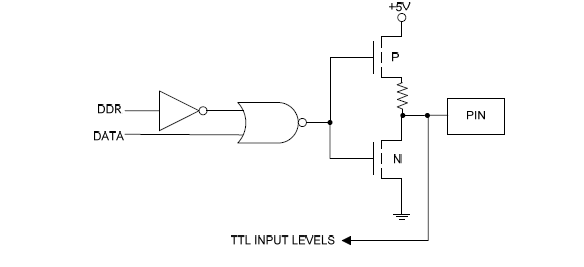
\includegraphics[scale=0.65]{images/via_pin_drivers.png}
    \end{center}
    \caption{VIA Pin Internal Circuitry}
    \label{fig:via_pin}
\end{figure}
\chapter{Game Controllers}

The \jr\ allows you to connect either Atari style joysticks or NES/SNES style gamepads as game controllers. The two different styles of controllers are used differently and are supported by different registers on the \jr. Note: Atari style analog devices are not supported ({\it e.g.} paddles, analog joysticks, analog mice).

\section*{Atari Style Joysticks}

The \jr\ has two IDC headers that can be connected to a DB-9 socket to allow Atari style joysticks to be used (see figure:~\ref{fig:joystick_ports} for the pinouts). Joystick header 0 is wired to the pins of Port B of the VIA (see page~\ref{chap_via}), and joystick header 1 is connected to Port A. The various joystick switches are connected to the ports in same manner as on the C-64, with the exception that more buttons are supported (see table:~\ref{tab:via_joystick}).

\begin{figure}[ht]
    \begin{center}
        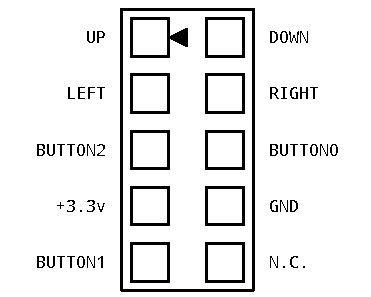
\includegraphics[scale=0.65]{images/f256_port_joystick.pdf}
    \end{center}
    \caption{Joystick Port Pinouts}
    \label{fig:joystick_ports}
\end{figure}

In order to use the joysticks, the DDR bits for the ports must be set to 0 for input. Then the input/output register for the port may be read. If a button or switch is closed on the joystick, the corresponding bit in the I/O register will be clear (0). If the button is not pressed, the bit will be set (1).

As a reminder: be aware that the WDC65C22 on the \jr\ is being used with a 3.3 volt supply. This means that any device plugged into the joystick ports should be 3.3 volt tolerant and should not raise any pin above 3.3 volts, otherwise damage could occur.

\begin{table}[ht]
    \begin{center}
        \begin{tabular}{|c|c|c|c|c|c|c|c|} \hline
            7 & 6 & 5 & 4 & 3 & 2 & 1 & 0 \\\hline\hline
            --- & BUTTON2 & BUTTON1 & BUTTON0 & RIGHT & LEFT & DOWN & UP \\ \hline
        \end{tabular}
    \end{center}
    \caption{Joystick Flags}
    \label{tab:via_joystick}
\end{table}

\example{Displaying Joystick 1}
In this example, we will poll joystick 1 and print out the state of all the buttons by printing the byte we read from the joystick port as a simple binary number. The example will try to be a little smart by only printing the value when the value has changed. NOTE: this example expects OpenKernal to be installed, and will call two of its routines for initializing the screen and printing a character.

First, we initialize the screen, the variable we use to track the old value of the joystick port, and the VIA (setting port A to be an input port):
\begin{verbatim}
ok_cint = $FF81                         ; OpenKernal: init the screen
ok_cout = $FFD2                         ; OpenKernal: print the character in A

; Variables

* = $0080

value:      .byte ?                     ; Variable to store the old joystick value
prv:        .byte ?                     ; Copy of value for printing

* = $e000

start:      jsr ok_cint                 ; Set up the screen

            lda #$FF                    ; Set the previous value to $FF
            sta value

            stz MMU_IO_CTRL             ; Switch to I/O Page 0

            lda #$00                    ; Set VIA Port A to input
            sta VIA_DDRA
\end{verbatim}

Next, we print the OpenKernal code to clear the screen, and we print out the byte in \verb+value+ as a binary number.

\begin{verbatim}
loop1:      lda #147                    ; Print the CBM clear screen code
            jsr ok_cout

            lda value                   ; Copy the value to prv
            sta prv

            ldx #8                      ; Loop for all eight bits
loop2:      asl prv                     ; Shift MSB into the carry
            bcc is0                     ; If it's 0, print '0'

            lda #'1'                    ; Otherwise, print '1'
            jsr ok_cout
            bra repeat                  ; And go to the next bit

is0:        lda #'0'                    ; Print '0'
            jsr ok_cout

repeat:     dex                         ; Count down
            bne loop2                   ; Repeat until we've done all 8 bits
\end{verbatim}

Next, we read the value of port A. If it is different from \verb+value+, we save it to \verb+value+ and go back to print the byte we read. Otherwise, we keep waiting and polling the joystick port.

\begin{verbatim}
            stz MMU_IO_CTRL             ; Switch to I/O Page 0

wait:       lda VIA_IORA                ; Get the status of port A
            cmp value                   ; Is it different from before?
            beq wait                    ; Yes: keep waiting

            sta value                   ; Save this value as the previous one
            bra loop1                   ; And go to print it
\end{verbatim}

\section*{NES/SNES Gamepads}

The \jr\ also provides support for NES/SNES compatible gamepads. NES gamepads work a little differently from Atari style joysticks. Where Atari style joysticks are directly readable through the VIA ports, NES gamepads communicate to the \jr\ through a serial interface. To read the gamepad, a program needs to first send the signal to the gamepad to capture the status of all the buttons, then the program needs to trigger the system to transfer the button status over the serial interface to the computer. This transfer takes a few clock cycles, since it is done serially, so the program needs to wait until the NES registers indicate that the transfer is done.

Before any transfer is done, the program must specify (by setting or clearing the MODE bit) whether the gamepad is NES compatible or SNES compatible. NES gamepads only send 8 bits of data, but SNES controllers send 12 bits. The NES/SNES data register are arranged differently depending on the value of MODE.

The process the program follows to read the state of the gamepad is:

\begin{enumerate}
    \item Set NES\_EN of NES\_CTRL to enable the NES/SNES support (see table~\ref{tab:nes_registers}) and set or clear MODE, to choose between NES mode or SNES mode.
    \item Set NES\_TRIG of NES\_CTRL to sample the buttons and transfer the data to the registers.
    \item Read NES\_STAT and wait until the DONE bit is set
    \item Check the appropriate NES or SNES control registers (see table~\ref{tab:nes_data_reg})
    \item Clear NES\_TRIG
\end{enumerate}

\begin{table}[ht]
    \begin{center}
        \begin{tabular}{|c|c|c|c|c|c|c|c|c|c|c|} \hline
            Address & R/W & Name & 7 & 6 & 5 & 4 & 3 & 2 & 1 & 0 \\\hline\hline
            \verb+0xD880+ & W & NES\_CTRL & NES\_TRIG & \multicolumn{4}{|c|}{---} & MODE & --- & NES\_EN \\ \hline
            \verb+0xD880+ & R & NES\_STAT & NES\_TRIG & DONE & \multicolumn{3}{|c|}{---} & MODE & --- & NES\_EN \\ \hline
        \end{tabular}
    \end{center}
    \caption{NES/SNES Gamepad Registers}
    \label{tab:nes_registers}
\end{table}

\begin{description}
    \item[NES\_CTRL] Set (1) to start the process of sampling the buttons.
    \item[DONE] If set (1), the gamepad status has been read into the registers, and is available for reading
    \item[MODE] If set (1), the gamepad is expected to be an SNES compatible controller. If clear (0), the gamepad is expected to be an NES compatible controller.
    \item[NES\_EN] If set (1), enables NES/SNES controller support.
\end{description}

\begin{table}[ht]
    \begin{center}
        \begin{tabular}{|c|c|c|c|c|c|c|c|c|c|c|} \hline
            MODE & Address & Pad & 7 & 6 & 5 & 4 & 3 & 2 & 1 & 0 \\\hline\hline
            \multirow{4}{*}{0} & 0xD884 & 0 & A & B & SELECT & START & UP & DOWN & LEFT & RIGHT \\\cline{2-11}
                & 0xD886 & 1 & A & B & SELECT & START & UP & DOWN & LEFT & RIGHT \\\cline{2-11}
                & 0xD888 & 2 & A & B & SELECT & START & UP & DOWN & LEFT & RIGHT \\\cline{2-11}
                & 0xD88A & 3 & A & B & SELECT & START & UP & DOWN & LEFT & RIGHT \\\hline\hline

            \multirow{8}{*}{1} & 0xD884 & \multirow{2}{*}{0} & B & Y & SELECT & START & UP & DOWN & LEFT & RIGHT \\\cline{2-2}\cline{4-11}
                               & 0xD885 &                    & \multicolumn{4}{|c|}{---} & A & X & L & R \\\cline{2-11}
                               & 0xD886 & \multirow{2}{*}{1} & B & Y & SELECT & START & UP & DOWN & LEFT & RIGHT \\\cline{2-2}\cline{4-11}
                               & 0xD887 &                    & \multicolumn{4}{|c|}{---} & A & X & L & R \\\cline{2-11}
                               & 0xD888 & \multirow{2}{*}{2} & B & Y & SELECT & START & UP & DOWN & LEFT & RIGHT \\\cline{2-2}\cline{4-11}
                               & 0xD889 &                    & \multicolumn{4}{|c|}{---} & A & X & L & R \\\cline{2-11}
                               & 0xD88A & \multirow{2}{*}{3} & B & Y & SELECT & START & UP & DOWN & LEFT & RIGHT \\\cline{2-2}\cline{4-11}
                               & 0xD88B &                    & \multicolumn{4}{|c|}{---} & A & X & L & R \\\hline
        \end{tabular}
    \end{center}
    \caption{NES/SNES Data Registers}
    \label{tab:nes_data_reg}
\end{table}

NOTE: If you want to use NES/SNES controllers with the \jr, you will need to add an adapter to convert the common port to NES and SNES connectors. The Foenix shop has the adapter, which comes in one of two flavors: one for the \jr\ (which has an IDC pin header on the board for the NES/SNES controollers), and one for the F256k (which has a 9 pin mini-DIN connector on the back).
\chapter{SD Card Interface}

TinyVicky includes an interface to the SD card port on \jr. This interface provides access to the SPI bus interface SD cards support. This interface will allow a program to exchange bytes of data with an SD card using one of two clock speeds for the transfer rate (400 kHz or 12.5 MHz).  Use of these registers requires an understanding of the SD card protocols and conventions, which are really outside the scope of this manual. So only the basic information about the control registers are provided here.

\begin{table}[ht]
    \begin{center}
        \begin{tabular}{|c|c|c|c|c|c|c|c|c|c|c|} \hline
            Address & R/W & 7 & 6 & 5 & 4 & 3 & 2 & 1 & 0 \\\hline\hline
            \verb+0xDD00+ & RW & SPI\_BUSY & \multicolumn{5}{|c|}{---} & SPI\_CLK & CS\_EN \\\hline
            \verb+0xDD01+ & RW & \multicolumn{8}{|c|}{SPI\_DATA} \\\hline
        \end{tabular}
    \end{center}
    \caption{SD Card Interface Registers}
\end{table}

\begin{description}
    \item[CS\_EN] This bit controls the chip select input on the SD card. If clear (0), the SD card is disabled. If set (1), the SD card is enabled.
    \item[SPI\_CLK] This bit controls the clock speed for the SPI interface to the SD card. If set (1), the clock speed is 400 kHz. If clear (0), the clock speed is 12.5 MHz.
    \item[SPI\_BUSY] This read only bit indicates if the SPI bus is busy exchanging bits with the SD card. The SPI\_DATA register will not be ready for access while SPI\_BUSY is set (1).
    \item[SPI\_DATA] this register is for the data to exchange with the SD card. A byte written to this register will be send to the SD card. The data read from this register are the bits received from the SD card. If SPI\_BUSY is set, the program must way until SPI\_BUSY is clear before reading or writing data to this register
\end{description}

NOTE: The system control registers have two bits relevant to the SD card interface: SD\_WP, which indicates the write-protect status of the card, and SD\_CD which indicates if a card is detected in the slot. See table~\ref{tab:sys_ctrl_reg} for details.
\chapter{Keyboard and Mouse}

The \jr\ provides a single PS/2 port for use with either a keyboard or a mouse. This port is accessed through five registers, which provide very simple access to a PS/2 device. The \jr\ does not have a full PS/2 controller, but instead provides mostly raw access to the data stream. It does make some attempt to translate set 2 scan codes to ASCII character code, although raw scan codes may be read instead. See table \ref{tab:ps2_reg} for details.

\begin{table}[ht]
    \begin{center}
        \begin{tabular}{|c|c|c|c|c|c|c|c|c|c|c|} \hline
            Address & R/W & Name & 7 & 6 & 5 & 4 & 3 & 2 & 1 & 0 \\\hline\hline
            \verb+0xD640+ & W & PS2\_CTRL & \multicolumn{2}{|c|}{---} & MCLR & KCLR & M\_WR & --- & K\_WR & --- \\\hline
            \verb+0xD641+ & W & PS2\_OUT & \multicolumn{8}{|l|}{Data to send to keyboard} \\ \hline
            \verb+0xD642+ & R & KBD\_IN & \multicolumn{8}{|l|}{Data from the keyboard input FIFO} \\ \hline
            \verb+0xD643+ & R & MS\_IN & \multicolumn{8}{|l|}{Data from the mouse input FIFO} \\ \hline
            \verb+0xD644+ & R & PS2\_STAT & K\_AK & K\_NK & M\_AK & M\_NK & \multicolumn{2}{|c|}{---} & MEMP & KEMP \\ \hline
        \end{tabular}
    \end{center}
    \caption{PS/2 Port Registers}
    \label{tab:ps2_reg}
\end{table}

\begin{description}
    \item[K\_WR] set to 1 then 0 to send a byte written on PS2\_OUT to the keyboard
    \item[M\_WR] set to 1 then 0 to send a byte written on PS2\_OUT to the mouse
    \item[KCLR] set to 1 then 0 to clear the keyboard input FIFO queue.
    \item[MCLR] set to 1 then 0 to clear the mouse input FIFO queue. 
    \item[K\_AK] when 1, the code sent to the keyboard has been acknowledged
    \item[K\_NK] when 1, the code sent to the keyboard has resulted in an error
    \item[M\_AK] when 1, the code sent to the keyboard has been acknowledged
    \item[M\_NK] when 1, the code sent to the keyboard has resulted in an error
    \item[KEMP] when 1, the keyboard input FIFO is empty
    \item[MEMP] when 1, the mouse input FIFO is empty 
\end{description}

\section*{Mouse Support}

The \jr\ provides special support for a PS/2 mouse, including support for a hardware mouse pointer.

This is currently done with magic, the details of which will be made apparent when the stars are in proper alignment.

\subsection*{Mouse Pointer}

The \jr\ provides for a grayscale hardware mouse pointer. The pointer is a $16 \times 16$ grayscale image of 256 levels. Each pixel of the image is a single byte. The bitmap data is stored in the address range 0xCC00--0xCFFF.

The position of the mouse pointer is controlled in one of two ways. In the default approach (MODE = 0), the system software will monitor mouse movements, determine the mouse position programmatically, and set the TinyVicky mouse position registers directly. In the legacy approach (MODE = 1), the system software will receive the three byte PS/2 mouse data packet and set the TinyVicky mouse PS2\_BYTE registers. In this legacy mode, TinyVicky will interpret the mouse packets and track the mouse position for the system. This approach is less work for the system software, but is less flexible.

\begin{table}[ht]
    \begin{center}
        \begin{tabular}{|c|c|c|c|c|c|c|c|c|c|} \hline
            Address & R/W & 7 & 6 & 5 & 4 & 3 & 2 & 1 & 0 \\\hline\hline
            \verb+0xD6E0+ & W & \multicolumn{6}{|c|}{---} & MODE & EN \\\hline
            \verb+0xD6E2+ & RW & X7 & X6 & X5 & X4 & X3 & X2 & X1 & X0 \\\hline
            \verb+0xD6E3+ & RW & X15 & X14 & X13 & X12 & X11 & X10 & X9 & X8 \\\hline
            \verb+0xD6E4+ & RW & Y7 & Y6 & Y5 & Y4 & Y3 & Y2 & Y1 & Y0 \\\hline
            \verb+0xD6E5+ & RW & Y15 & Y14 & Y13 & Y12 & Y11 & Y10 & Y9 & Y8 \\\hline
            \verb+0xD6E6+ & W & \multicolumn{8}{|c|}{PS2\_BYTE\_0} \\\hline
            \verb+0xD6E7+ & W & \multicolumn{8}{|c|}{PS2\_BYTE\_1} \\\hline
            \verb+0xD6E8+ & W & \multicolumn{8}{|c|}{PS2\_BYTE\_2} \\\hline
        \end{tabular}
    \end{center}
    \caption{Mouse Pointer Registers}
    \label{tab:mouse_reg}
\end{table}

\begin{description}
    \item[EN] if set (1), the mouse pointer is displayed. If clear (0), the mouse pointer is not displayed
    \item[MODE] if clear (0), the mouse position is specified by setting the X and Y registers. If set (1), the program must pass along the 3 byte PS/2 mouse packet to the packet registers (this is a legacy mode).
    \item[X] this is the X coordinate of the mouse and both readable and writable if MODE is clear (0)
    \item[Y] this is the Y coordinate of the mouse and both readable and writable if MODE is clear (0)
    \item[PS2\_BYTE\_0] the first byte of the PS/2 mouse message packet. Only used if MODE is set (1).
    \item[PS2\_BYTE\_1] the second byte of the PS/2 mouse message packet. Only used if MODE is set (1).
    \item[PS2\_BYTE\_2] the third byte of the PS/2 mouse message packet. Only used if MODE is set (1).
\end{description}

\section*{F256K Keyboard}
\label{sec_f256k_kbd}

\begin{leftbar}
    NOTE: this section pertains to the F256K only and is not relevant to the \jr.
\end{leftbar}

The F256K includes a second WDC65C22 VIA chip at 0xDB00 on I/O page 0 (see page \pageref{chap_via} for details on the VIAs) which manages the keyboard input from the F256K's built-in keyboard. The F256K's keyboard is a matrix keyboard. Except for the RESTORE key, all keys on the keyboard are arranged in a matrix with the columns assigned to VIA1's PB pins and the rows assigned to VIA1's PA pins. VIA0's PB7 pin is also used for a column. See figure~\ref{fig:f256k_matrix}.

\begin{figure}[ht]
    \begin{center}
        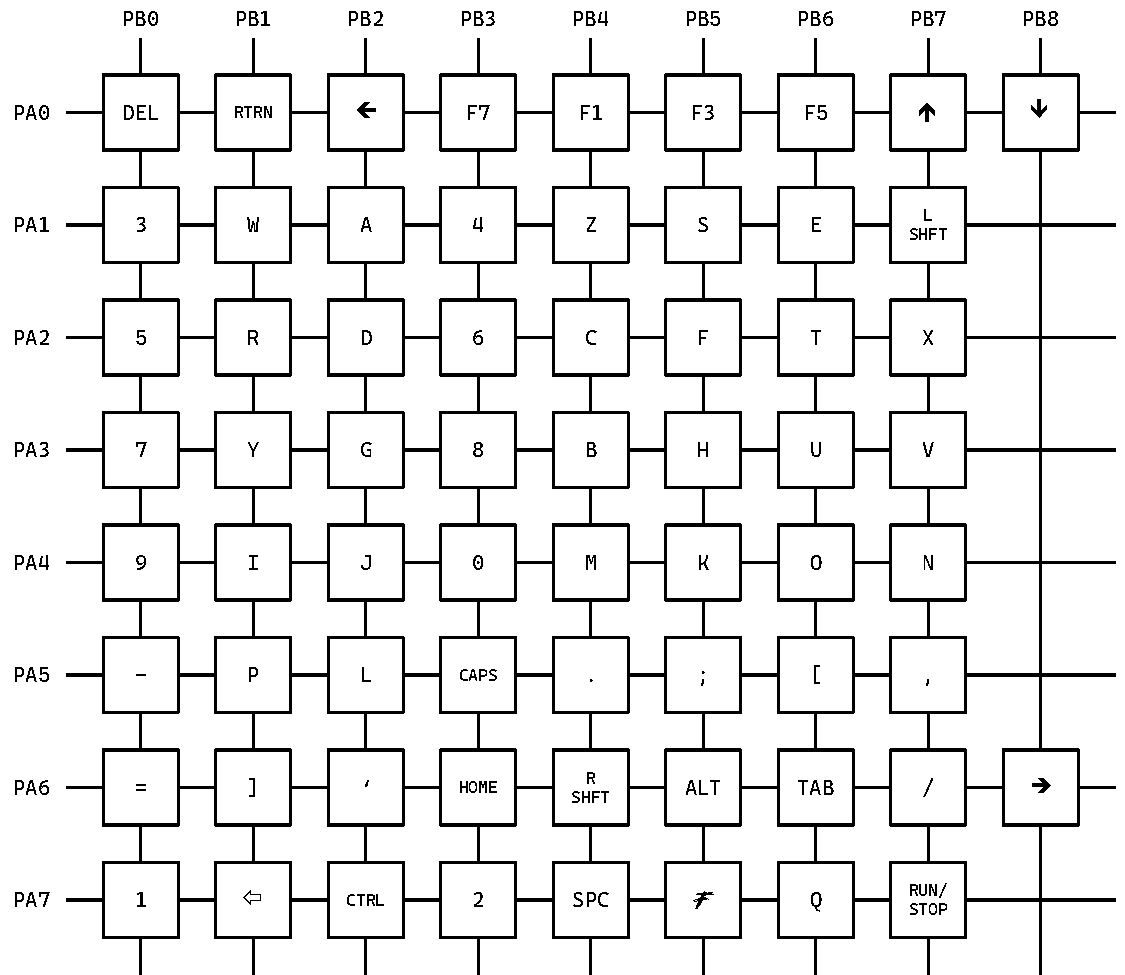
\includegraphics[scale=0.5]{images/f256k_matrix.pdf}
    \end{center}
    \caption{F256K Keyboard Matrix}
    \label{fig:f256k_matrix}
\end{figure}


\chapter{Serial and Wi-Fi Port}

The \jr\ has a simple UART for serial communications. This UART can be used to provide an RS-232 serial connection (via an IDC header on the board compatible with IDC to DB-9 cables) or a Wi-Fi serial connection using an ESP8266 Feather adapter board. The UART is compatible with the standard 16750.

\begin{table}[ht]
    \begin{center}
        \begin{tabular}{|c|c|c|c|c|c|c|c|c|c|c|} \hline
            Address & R/W & Name & 7 & 6 & 5 & 4 & 3 & 2 & 1 & 0 \\\hline\hline
            \multicolumn{11}{|c|}{DLAB = 0} \\ \hline
            \verb+0xD630+ & R & RXD & \multicolumn{8}{|c|}{RX\_DATA} \\ \hline
            \verb+0xD630+ & W & TXR & \multicolumn{8}{|c|}{TX\_DATA} \\ \hline
            \verb+0xD631+ & R/W & IER & \multicolumn{4}{|c|}{---} & STAT & ERR & TXE & RXA \\ \hline
            \verb+0xD632+ & R & ISR & \multicolumn{4}{|c|}{---} & STAT & ERR & TXE & RXA \\ \hline
            \verb+0xD632+ & W & FCR & \multicolumn{2}{|c|}{RXT} & FIFO64 & --- & --- & TXR & RXR & FIFOE \\ \hline
            \verb+0xD633+ & R/W & LCR & DLAB & --- & \multicolumn{3}{|c|}{PARITY} & STOP & \multicolumn{2}{|c|}{DATA} \\ \hline
            \verb+0xD634+ & R/W & MCR & \multicolumn{3}{|c|}{---} & LOOP & OUT2 & OUT1 & RTS & DTR \\ \hline
            \verb+0xD635+ & R & LSR & ERR & TEMT & THRE & BI & FE & PE & OE & DR \\ \hline
            \verb+0xD636+ & R/W & MSR & DCD & RI & DSR & CTS & DDCD & TERI & DDSR & DCTS \\ \hline
            \verb+0xD637+ & R & SPR & \multicolumn{8}{|c|}{scratch data} \\ \hline\hline

            \multicolumn{11}{|c|}{DLAB = 1} \\ \hline
            \verb+0xD630+ & R/W & DLL & DIV7 & DIV6 & DIV5 & DIV4 & DIV3 & DIV2 & DIV1 & DIV0 \\ \hline
            \verb+0xD631+ & R/W & DLH & DIV15 & DIV14 & DIV13 & DIV12 & DIV11 & DIV10 & DIV9 & DIV8 \\ \hline
            \verb+0xD632+ & W & PSD & \multicolumn{8}{|c|}{prescaler division} \\ \hline
        \end{tabular}
    \end{center}
    \caption{UART Registers}
    \label{tab:uart_reg}
\end{table}

\begin{description}
    \item[RXD] (read only) register contains data from the receive FIFO

    \item[TXR] (write only) writing a byte stores it in the transmission FIFO to be sent over the serial connection

    \item[IER] this is the interrupt enable register. There are flags for each of the four conditions that the UART can use to trigger an interrupt

    \item[ISR] this is the interrupt STAT register. There are flags for each of the four conditions that can trigger an interrupt

    \item[FCR] FIFO control register. This register controls the FIFOs for transmission and receiving:
        \begin{description}
            \item[RXT] sets the number of characters in the receive FIFO to trigger an interrupt. See table:~\ref{tab:uart_rx_trig}.

            \item[FIFO64] enables the 64 byte FIFO

            \item[TXR] if set, clear the transmition FIFO

            \item[RXR] if set, clear the receive FIFO

            \item[FIFOE] if set, the FIFOs are enabled. Otherwise, only a single character can be waiting to send or pending a read
        \end{description}
\end{description}

\begin{table}[ht]
    \begin{center}
        \begin{tabular}{|c|c|c|} \hline
            LCR1 & LCR0 & Length \\ \hline\hline
            0 & 0 & 5 \\ \hline
            0 & 1 & 6 \\ \hline
            1 & 0 & 7 \\ \hline
            1 & 1 & 8 \\ \hline
        \end{tabular}
    \end{center}
    \caption{UART Data Length}
    \label{tab:uart_data}
\end{table}

\begin{table}[ht]
    \begin{center}
        \begin{tabular}{|c|c|} \hline
            LCR2 & Stop Bits \\ \hline\hline
            0 & 1 \\ \hline
            1 & 1.5 or 2 \\ \hline
        \end{tabular}
    \end{center}
    \caption{UART Stop Bits}
    \label{tab:uart_stop}
\end{table}

\begin{table}[ht]
    \begin{center}
        \begin{tabular}{|c|c|c|c|} \hline
            LCR5 & LCR4 & LCR3 & Parity \\ \hline\hline
            --- & --- & 0 & NONE \\ \hline
            0 & 0 & 1 & ODD \\ \hline
            0 & 1 & 1 & EVEN \\ \hline
            1 & 0 & 1 & MARK \\ \hline
            1 & 1 & 1 & SPACE \\ \hline
        \end{tabular}
    \end{center}
    \caption{UART Parity}
    \label{tab:uart_parity}
\end{table}

\begin{table}[ht]
    \begin{center}
        \begin{tabular}{|c|c|c|} \hline
            FCR7 & FCR6 & Trigger Level (bytes) \\ \hline\hline
            0 & 0 & 1 \\ \hline
            0 & 1 & 4 \\ \hline
            1 & 0 & 8 \\ \hline
            1 & 1 & 14 \\ \hline
        \end{tabular}
    \end{center}
    \caption{UART RX FIFO Trigger}
    \label{tab:uart_rx_trig}
\end{table}

\begin{table}[ht]
    \begin{center}
        \begin{tabular}{|c|c|c|} \hline
            BPS & Divisor \\ \hline\hline
            300 & 5,244 \\ \hline
            600 & 2,622 \\ \hline
            1,200 & 1,311 \\ \hline
            1,800 & 874 \\ \hline
            2,000 & 786 \\ \hline
            2,400 & 655 \\ \hline
            3,600 & 437 \\ \hline
            4,800 & 327 \\ \hline
            9,600 & 163 \\ \hline
            19,200 & 81 \\ \hline
            38,400 & 40 \\ \hline
            57,600 & 27 \\ \hline
            115,200 & 13 \\ \hline
        \end{tabular}
    \end{center}
    \caption{UART Divisors}
    \label{tab:uart_divisors}
\end{table}


\chapter{Direct Memory Access}

The DMA engine can either write a specific byte to RAM or copy a set of bytes from one location in RAM to another. The DMA engine can also treat memory as being arranged either linearly (that is, as a certain number of consecutive locations) or as a rectangle (the data is a rectangular area of an image).

\section*{Linear Data}
Linear data (or ``1D'', if you prefer) is just a single block of sequential memory locations. When filling or copying data linearly, you need a destination address (and a source address if copying), and a count of bytes to copy. That is really all there is to it.

\section*{Rectangular Data}
Rectangular data (or ``2D'') is a bit more complicated and is meant to be working with image data. With a bitmap, the pixel bytes are arranged in memory left to right and top to bottom. If the image starts at address $a$ and is $w$ pixels wide, then the pixel at $(x, y)$ can be found at location $a + y \times w + x$. Rectangular fills and copies are meant to work on data that is arranged in this fashion. In this case, you can use DMA to fill or copy a rectangular area within that image. As with linear fills and copies, you will need a destination address (and source address if doing a copy), but instead of a count of bytes you need the width and height of the rectangular areas affected. But you need one other thing, too. You need to tell the DMA the geometry of the over-all image... you need to tell it the width of the image containing the rectangular areas. This is called the ``stride'' and effectively tells the DMA how many pixels to skip between lines when it finishes one line of the rectangle before getting to the next line.

\begin{table}[ht]
    \begin{center}
        \begin{tabular}{|c|c|c|c|c|c|c|c|c|c|} \hline
            Address & R/W & 7 & 6 & 5 & 4 & 3 & 2 & 1 & 0 \\\hline\hline
            \verb+0xDF00+ & R/W & START & \multicolumn{3}{|c|}{---} & INT\_EN & FILL & 2D & ENABLE \\ \hline
            \verb+0xDF01+ & W & FD7 & FD6 & FD5 & FD4 & FD3 & FD2 & FD1 & FD0 \\ \hline
            \verb+0xDF01+ & R & BUSY & \multicolumn{7}{|c|}{---}  \\ \hline\hline

            \verb+0xDF04+ & R/W & SA7 & SA6 & SA5 & SA4 & SA3 & SA2 & SA1 & SA0 \\ \hline
            \verb+0xDF05+ & R/W & SA15 & SA14 & SA13 & SA12 & SA11 & SA10 & SA9 & SA8 \\ \hline
            \verb+0xDF06+ & R/W & \multicolumn{6}{|c|}{---} & SA17 & SA16 \\ \hline\hline

            \verb+0xDF08+ & R/W & DA7 & DA6 & DA5 & DA4 & DA3 & DA2 & DA1 & DA0 \\ \hline
            \verb+0xDF09+ & R/W & DA15 & DA14 & DA13 & DA12 & DA11 & DA10 & DA9 & DA8 \\ \hline
            \verb+0xDF0A+ & R/W & \multicolumn{6}{|c|}{---} & DA17 & DA16 \\ \hline
        \end{tabular}
    \end{center}
    \caption{DMA Registers (Part 1)}
    \label{tab:dma_reg}
\end{table}

\begin{table}[ht]
    \begin{center}
        \begin{tabular}{|c|c|c|c|c|c|c|c|c|c|} \hline
            Address & R/W & 7 & 6 & 5 & 4 & 3 & 2 & 1 & 0 \\\hline\hline
            \verb+0xDF0C+ & R/W & CNT7 & CNT6 & CNT5 & CNT4 & CNT3 & CNT2 & CNT1 & CNT0 \\ \hline
            \verb+0xDF0D+ & R/W & CNT15 & CNT14 & CNT13 & CNT12 & CNT11 & CNT10 & CNT9 & CNT8 \\ \hline
            \verb+0xDF0E+ & R/W & \multicolumn{6}{|c|}{---} & CNT17 & CNT16 \\ \hline\hline

            \verb+0xDF0C+ & R/W & W7 & W6 & W5 & W4 & W3 & W2 & W1 & W0 \\ \hline
            \verb+0xDF0D+ & R/W & W15 & W14 & W13 & W12 & W11 & W10 & W9 & W8 \\ \hline
            \verb+0xDF0E+ & R/W & H7 & H6 & H5 & H4 & H3 & H2 & H1 & H0 \\ \hline
            \verb+0xDF0F+ & R/W & H15 & H14 & H13 & H12 & H11 & H10 & H9 & H8 \\ \hline\hline

            \verb+0xDF10+ & R/W & SS7 & SS6 & SS5 & SS4 & SS3 & SS2 & SS1 & SS0 \\ \hline
            \verb+0xDF11+ & R/W & SS15 & SS14 & SS13 & SS12 & SS11 & SS10 & SS9 & SS8 \\ \hline

            \verb+0xDF12+ & R/W & SD7 & SD6 & SD5 & SD4 & SD3 & SD2 & SD1 & SD0 \\ \hline
            \verb+0xDF13+ & R/W & SD15 & SD14 & SD13 & SD12 & SD11 & SD10 & SD9 & SD8 \\ \hline
        \end{tabular}
    \end{center}
    \caption{DMA Registers (Part 2)}
    \label{tab:dma_reg_2}
\end{table}


\begin{description}
    \item[START] set to trigger the DMA

    \item[INT\_EN] enables triggering an interrupt when DMA is complete

    \item[FILL] when set, DMA will write a specific byte to memory. When clear, DMA will copy data from a source address to the destination address

    \item[2D] when set, DMA copies or fills a rectangular region of memory. When clear, DMA copies or fills a certain number of sequential bytes

    \item[ENABLE] set to enable DMA

    \item[FD] the byte to be written to memory when FILL is set

    \item[BUSY] status bit set when DMA is busy copying data

    \item[SA] the 18 bit source address (must be a location in the first 256KB of RAM). Only relevant when FILL is clear.

    \item[DA] the 18 bit destination address (must be a location in the first 256KB of RAM)

    \item[CNT] the number of bytes to copy (only available when 2D is clear)

    \item[W] the width of the rectangle of data to copy (only available when 2D is set)

    \item[H] the height of the rectangle of data to copy (only available when 2D is set)

    \item[SS] the width of the ``stride'' for the source bitmap (only available for 2D copy operations)

    \item[SD] the width of the ``stride'' for the destination bitmap (only available when 2D is set)
\end{description}

The term ``stride'' might be a little confusing. It is a concept only relevant for 2D DMA operations. For 2D operations, the DMA engine is always copying or filling a rectangular area of a given width and height. The width of the rectangle need not be the full size of the overall bitmap image. If a program performs a DMA operation on a $32 \times 32$ area of the screen, the DMA engine will need to skip many pixels on each affected line. Thus, the program needs to inform the DMA engine how many pixels wide the bitmap is. For example, if a program is filling $32 \times 32$ rectangle in a $320 \times 240$ bitmap, it needs to tell the DMA engine that the width of the bitmap is 320. This number is the ``stride'' for the operation. The DMA engine will operate on 32 pixels, then skip $320 - 32$ pixels to get to the next set of 32 pixels to copy or fill. Figure~\ref{fig:dma_2d} illustrates how the various addresses, sizes, and strides work in the case of a 2D copy operation.

For 2D fill operations, only the destination stride (SD) is needed. The destination stride specifies how wide the bitmap being altered is. For 2D copy operations, both the destination stride and the source stride (SS) are needed. The source stride specifies how wide the bitmap is that provides the source data. Why would you ever have a source and destination stride be different? As a simple example, let's say a program needs to copy graphical font data to a bitmap for the screen in $320 \times 240$ mode. The characters are in cells that are 8 pixels wide by 16 pixels deep, and that the characters are arranged vertically. So the over all image for the characters is 8 pixels wide by 4,096 pixels high. In that case, the source stride is 8, but the destination stride is 320 (since it is the bitmap for the full screen).

\begin{figure}[ht]
    \begin{center}
        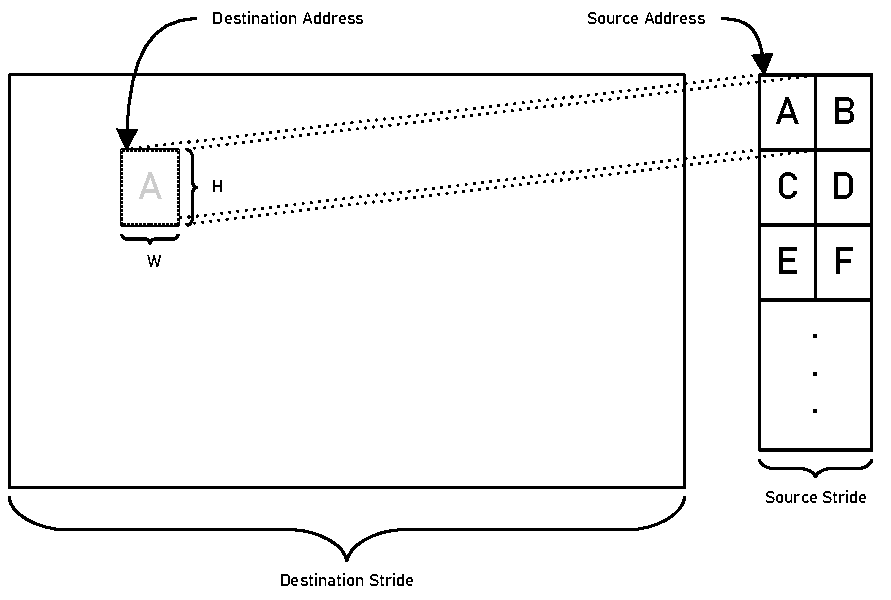
\includegraphics[scale=0.75]{images/f256_dma_2d.pdf}
    \end{center}
    \caption{A 2D Copy DMA Operation}
    \label{fig:dma_2d}
\end{figure}


\example{Using DMA to Fill a Bitmap}
\label{ex:dma}

In this example, we will use the 1D fill operation to set the bitmap shown on the screen to a set color. Note that the full example code includes the various setup operations for the bitmap mode and the graphics CLUTs, which are exactly the same as were used in the bitmap example (see page~\ref{ex:bitmap}).

\begin{verbatim}
DMA_CTRL = $DF00                ; DMA Control Register
DMA_CTRL_START = $80            ; Start the DMA operation
DMA_CTRL_FILL = $04             ; DMA is a fill operation
DMA_CTRL_ENABLE = $01           ; DMA engine is enabled

DMA_STATUS = $DF01              ; DMA status register (Read Only)
DMA_STAT_BUSY = $80             ; DMA engine is busy with an operation

DMA_FILL_VAL = $DF01            ; Byte value to use for fill operations

DMA_DST_ADDR = $DF08            ; Destination address (system bus)
DMA_COUNT = $DF0C               ; Number of bytes to fill or copy

bitmap_base = $10000            ; The base address of our bitmap

bitmap_width = 320              ; The size of our bitmap
bitmap_height = 240
bitmap_size = bitmap_width*bitmap_height
\end{verbatim}

First, we need to enable the DMA engine and set it up for a fill operation:

\begin{verbatim}
            lda #DMA_CTRL_FILL | DMA_CTRL_ENABLE
            sta DMA_CTRL
\end{verbatim}

Next, we provide the value to fill:

\begin{verbatim}
            lda #$ff
            sta DMA_FILL_VAL    ; We will fill the screen with $FF
\end{verbatim}

Then we need to provide the destination address:

\begin{verbatim}
            lda #<bitmap_base   ; Our bitmap will be the destination
            sta DMA_DST_ADDR
            lda #>bitmap_base
            sta DMA_DST_ADDR+1
            lda #`bitmap_base
            and #$03
            sta DMA_DST_ADDR+2
\end{verbatim}

Next, we provide the number of bytes to write:

\begin{verbatim}
            lda #<bitmap_size   ; We will write 320*240 bytes
            sta DMA_COUNT
            lda #>bitmap_size
            sta DMA_COUNT+1
            lda #`bitmap_size
            sta DMA_COUNT+2
\end{verbatim}

Finally, we flip the START flag to trigger the DMA operation and wait for it to complete:

\begin{verbatim}
            lda DMA_CTRL
            ora #DMA_CTRL_START
            sta DMA_CTRL

wait_dma:   lda DMA_STATUS      ; Wait until DMA is not busy
            and #DMA_STAT_BUSY
            cmp #DMA_STAT_BUSY
            beq wait_dma

            stz DMA_CTRL        ; Turn off the DMA engine
\end{verbatim}

\example{Calculating an Address for DMA}
\label{ex:dma_2d}

We can extend our 1D DMA example to draw a 2D rectangle at a given coordinate on the screen. Using the coordinate math block, we can quickly calculate the starting address for the destination address of the rectangle to fill.

\begin{verbatim}
DMA_CTRL_2D = $02               ; DMA is 2D operation (otherwise it is 1D)

DMA_WIDTH = $DF0C               ; Width of rectangle to fill or copy
DMA_HEIGHT = $DF0E              ; Height of rectangle to fill or copy

DMA_STRIDE_DST = $DF12          ; Width of the destination bitmap image

XY_BASE = $D301         ; Starting address of the bitmap
XY_POS_X = $D304        ; X-coordinate desired
XY_POS_Y = $D306        ; Y-coordinate desired
XY_OFFSET = $D308       ; Offset within an MMU bank of the pixel for (X, Y)
XY_BANK = $D30A         ; MMU bank containing the pixel for (X, Y)
XY_ADDRESS = $D30B      ; System address of the pixel for (X, Y)
\end{verbatim}

We start off very similar to the 1D fill and just turn on the flag for 2D DMA:
\begin{verbatim}
    lda #DMA_CTRL_FILL | DMA_CTRL_2D | DMA_CTRL_ENABLE
    sta DMA_CTRL
\end{verbatim}

Now, we can take the base address of our bitmap and use it at the base address of the coordinate calculation:

\begin{verbatim}
    lda #<bitmap_base   ; Give the coordinate math unit the base address
    sta XY_BASE
    lda #>bitmap_base
    sta XY_BASE+1
    lda #`bitmap_base
    and #$03
    sta XY_BASE+2
\end{verbatim}

Next, we give it our $x$ and $y$ coordinates for the upper left corner of the rectangle we want to draw. In this case, $(100, 40)$:

\begin{verbatim}
    lda #100             ; Set (x,y) of the rectangle to (100, 40)
    sta XY_POS_X    
    stz XY_POS_X+1
    lda #40
    sta XY_POS_Y
    stz XY_POS_Y+1
\end{verbatim}

Then, we can just read off the address from the coordinate calculator and use it as the destination address for our DMA operation:

\begin{verbatim}
    lda XY_ADDRESS      ; Get the address of the upper left corner of the rect
    sta DMA_DST_ADDR    ; And use it as the DMA address
    lda XY_ADDRESS+1
    sta DMA_DST_ADDR+1
    lda XY_ADDRESS+2
    sta DMA_DST_ADDR+2

    lda #$30
    sta DMA_FILL_VAL    ; We will fill the screen with $30     
\end{verbatim}

A difference from 1D is that the size of the fill is a width and a height, so we provide the width and height of the rectangle we want to draw. In this case, we are setting it to $(100, 30)$:

\begin{verbatim}
    lda #100            ; Size of rectangle is (100,30)
    sta DMA_WIDTH
    stz DMA_WIDTH+1
    lda #30
    sta DMA_HEIGHT
    stz DMA_HEIGHT+1
\end{verbatim}

For 2D DMA operations, we need to provide the ``stride''. This is the width of the overall bitmap into which the DMA operation is writing. In this case, we are updating a bitmap that is the full screen, so we set the destination stride to 320:

\begin{verbatim}
    lda #<bitmap_width  ; Set the width of the destination bitmap for 2D DMA
    sta DMA_STRIDE_DST
    lda #>bitmap_width
    sta DMA_STRIDE_DST+1
\end{verbatim}

And then we can start the DMA operation and wait for it to complete:

\begin{verbatim}
    lda DMA_CTRL
    ora #DMA_CTRL_START
    sta DMA_CTRL

wait_dma2d: lda DMA_STATUS      ; Wait until DMA is not busy
    and #DMA_STAT_BUSY
    cmp #DMA_STAT_BUSY
    beq wait_dma2d
\end{verbatim}
\chapter{System Control Registers}
\label{sec:sysctrl}

\section*{The Buzzer and Status LEDs}

The \jr\ has several software-controllable LEDs. There are the SD card access LED and the power LED, but there are also two status LEDs on the board which may be controlled either manually or set to flash automatically. All the LEDs under ``manual'' control can be controlled by setting or clearing their relevant flags in the SYS0 register (0xD6A0) (see table:~\ref{tab:sys_ctrl_reg}). The power LED is controlled by PWR\_LED. The SD card LED is controlled by SD\_LED.

\begin{table}[ht]
    \begin{center}
        \begin{tabular}{|c|c|c|c|c|c|c|c|c|c|c|} \hline
            Address & R/W & Name & 7 & 6 & 5 & 4 & 3 & 2 & 1 & 0 \\\hline\hline

            \verb+0xD6A0+ & W & SYS0 & RESET & --- & CAP\_EN & BUZZ & L1 & L0 & SD\_L & PWR\_L \\ \hline
            \verb+0xD6A0+ & R & SYS0 & --- & SD\_WP & SD\_CD & BUZZ & L1 & L0 & SD\_L & PWR\_L \\ \hline
            \verb+0xD6A1+ & R/W & SYS1 & \multicolumn{2}{|c|}{L1\_RATE}
                                       & \multicolumn{2}{|c|}{L0\_RATE}
                                       & SID\_ST
                                       & PSG\_ST
                                       & L1\_MN & L0\_MN \\ \hline
        \end{tabular}
    \end{center}
    \caption{System Control Registers}
    \label{tab:sys_ctrl_reg}
\end{table}

The two status LEDs on the board are a little more complex. They may be in manual or automatic mode. The two flags L0\_MN and L1\_MN in SYS1 control which mode they are in. If an LED's flag is set (1), then the LED is under manual control and its equivalent flag in SYS0 controls whether the LED is on or off. If the flag is clear, then the LED is set to flash automatically, and the LED's flashing rate will be set by pair of bits L0\_RATE or L1\_RATE according to table~\ref{tab:led_rates}.

The flag PSG\_ST controls how the output of the PSG sound chips are mixed. If clear (0), the PSGs will be mixed for monaural output (both will go to both left and right channels). If set (1), the left PSG will go to the left channel, and the right PSG will go to the right channel. This allows a program to use the PSGs as either independent 4 voice channels in stereo or as a monaural 8 voice channels.

The flag SID\_ST controls how the output of the SID devices are mixed. If clear (0), the SIDs will be mixed for monaural output (both will go to both left and right channels). If set (1), the left SID will go to the left channel, and the right SID will go to the right channel. This allows a program to use the SIDs as either independent 4 voice channels in stereo or as a monaural 8 voice channels.

For the PC speaker, there is the BUZZ flag. By toggling BUZZ, a program can tweak the speaker and make a noise.

\begin{note}
    CAP\_EN is only on the \fk. If set, it enables the RGB LED for the shift lock key. It is ignored on the \jr.
    Likewise, the \fk\ does not have a built-in buzzer, so BUZZ is ignored on the \fk. The SID\_ST flag is also available on the \fk\ only. The same functionality is provided by jumpers on the \fjr\ board.
\end{note}

\begin{table}[ht]
    \begin{center}
        \begin{tabular}{|c|c|c|} \hline
            RATE1 & RATE0 & Rate \\\hline\hline
            0 & 0 & 1s \\ \hline
            0 & 1 & 0.5s \\ \hline
            1 & 0 & 0.4s \\ \hline
            1 & 1 & 0.2s \\ \hline
        \end{tabular}
    \end{center}
    \caption{LED Flash Rates}
    \label{tab:led_rates}
\end{table}

\section*{Software Reset}

A program can trigger a system reset. This can be done by writing the value \verb+0xDE+ to \verb+0xD6A2+ and the value \verb+AD+ to \verb+0xD6A3+ to validate that a reset is really intended (see table:~\ref{tab:sys_reset}), setting the most significant bit (RESET) of \verb+0xD6A0+, and then clearing the RESET bit to actually trigger the reset.

\begin{table}[ht]
    \begin{center}
        \begin{tabular}{|c|c|c|c|c|c|c|c|c|c|c|} \hline
            Address & R/W & Name & 7 & 6 & 5 & 4 & 3 & 2 & 1 & 0 \\\hline\hline
            \verb+0xD6A2+ & R/W & RST0 & \multicolumn{8}{|c|}{Set to 0xDE to enable software reset} \\ \hline
            \verb+0xD6A3+ & R/W & RST1 & \multicolumn{8}{|c|}{Set to 0xAD to enable software reset} \\ \hline
        \end{tabular}
    \end{center}
    \caption{System Reset}
    \label{tab:sys_reset}
\end{table}

\section*{Random Numbers}

The \jr\ has a built-in pseudo-random number generator that produces 16-bit random numbers (see table:~\ref{tab:rng_reg}). To use the random number generator, a program just sets the enable flag and then reads the random numbers from RNDL and RNDH (0xD6A4 and 0xD6A5). The program can set the seed value to better randomize the numbers by storing a seed value in those same locations and then toggling SEED\_LD (set to load the seed value then reclear).

\begin{table}[ht]
    \begin{center}
        \begin{tabular}{|c|c|c|c|c|c|c|c|c|c|c|} \hline
            Address & R/W & Name & 7 & 6 & 5 & 4 & 3 & 2 & 1 & 0 \\\hline\hline
            \verb+0xD6A4+ & W & SEEDL & \multicolumn{8}{|c|}{SEED[7\ldots 0]} \\ \hline
            \verb+0xD6A4+ & R & RNDL & \multicolumn{8}{|c|}{RND[7\ldots 0]} \\ \hline
            \verb+0xD6A5+ & W & SEEDH & \multicolumn{8}{|c|}{SEED[15\ldots 0]} \\ \hline
            \verb+0xD6A5+ & R & RNDH &  \multicolumn{8}{|c|}{RND[15\ldots 0]} \\ \hline

            \verb+0xD6A6+ & W & RND\_CTRL & \multicolumn{6}{|c|}{---} & SEED\_LD & ENABLE \\ \hline
            \verb+0xD6A6+ & R & RND\_STAT & DONE & \multicolumn{7}{|c|}{---} \\ \hline

        \end{tabular}
    \end{center}
    \caption{Random Number Generator}
    \label{tab:rng_reg}
\end{table}

\begin{description}
    \item[ENABLE] set to turn on the random number generator

    \item[SEED\_LD] set to load a value stored in SEEDL and SEEDH as the seed value for the random number generator

    \item[RNDL and RNDH] read 16-bit random numbers from these registers when the random number generator is enabled
\end{description}

\section*{Machine ID and Version Information}

Nine registers are set aside to identify the machine, the version of the printed circuit board, and the version of the FPGA. See table~\ref{tab:machine_id_ver} for the various registers. All the registers are read-only, and only the chip information will change over the course of the machine's life span. The machine ID contains a four-bit code that is common between all the Foenix machines (see table~\ref{tab:machine_ids}).

For the \jr, the machine ID will be 0x02. For the \fk, the machine ID will be 0x12.

\begin{table}[ht]
    \begin{center}
        \begin{tabular}{|c|c|c|c|c|c|c|c|c|c|c|} \hline
            Address & R/W & Name & 7 & 6 & 5 & 4 & 3 & 2 & 1 & 0 \\\hline\hline
            \verb+0xD6A7+ & R & MID & \multicolumn{3}{|c|}{---} & \multicolumn{5}{|c|}{ID} \\ \hline\hline

            \verb+0xD6A8+ & R & PCBID0 & \multicolumn{8}{|c|}{ASCII character 0: ``B''} \\ \hline
            \verb+0xD6A9+ & R & PCBID1 & \multicolumn{8}{|c|}{ASCII character 1: ``0''} \\ \hline
            \verb+0xD6AA+ & R & CHSV0 & \multicolumn{8}{|c|}{TinyVicky subversion in BCD (low)} \\ \hline
            \verb+0xD6AB+ & R & CHSV1 & \multicolumn{8}{|c|}{TinyVicky subversion in BCD (high)} \\ \hline
            \verb+0xD6AC+ & R & CHV0 & \multicolumn{8}{|c|}{TinyVicky version in BCD (low)} \\ \hline
            \verb+0xD6AD+ & R & CHV1 & \multicolumn{8}{|c|}{TinyVicky version in BCD (high)} \\ \hline
            \verb+0xD6AE+ & R & CHN0 & \multicolumn{8}{|c|}{TinyVicky number in BCD (low)} \\ \hline
            \verb+0xD6AF+ & R & CHN1 & \multicolumn{8}{|c|}{TinyVicky number in BCD (high)} \\ \hline\hline

            \verb+0xD6EB+ & R & PCBMA & \multicolumn{8}{|c|}{PCB Major Rev (ASCII)} \\ \hline
            \verb+0xD6EC+ & R & PCBMI & \multicolumn{8}{|c|}{PCB Minor Rev (ASCII)} \\ \hline
            \verb+0xD6ED+ & R & PCBD & \multicolumn{8}{|c|}{PCB Day (BCD)} \\ \hline
            \verb+0xD6EE+ & R & PCBM & \multicolumn{8}{|c|}{PCB Month (BCD)} \\ \hline
            \verb+0xD6EF+ & R & PCBY & \multicolumn{8}{|c|}{PCB Year (BCD)} \\ \hline
        \end{tabular}
    \end{center}
    \caption{Machine ID and Versions}
    \label{tab:machine_id_ver}
\end{table}

\begin{table}[ht]
    \begin{center}
        \begin{tabular}{|c|c|c|c|c|c|} \hline
            MID4 & MID3 & MID2 & MID1 & MID0 & Machine \\\hline\hline
            0 & 0 & 0 & 0 & 0 & C256 FMX \\ \hline
            0 & 0 & 0 & 0 & 1 & C256 U \\ \hline
            0 & 0 & 0 & 1 & 0 & \jr \\ \hline
            1 & 0 & 0 & 1 & 0 & \fk \\ \hline
            0 & 0 & 0 & 1 & 1 & A2560 Dev \\ \hline
            0 & 0 & 1 & 0 & 0 & Gen X \\ \hline
            0 & 0 & 1 & 0 & 1 & C256 U+ \\ \hline
            0 & 0 & 1 & 1 & 0 & Reserved \\ \hline
            0 & 0 & 1 & 1 & 1 & Reserved \\ \hline
            0 & 1 & 0 & 0 & 0 & A2560 X \\ \hline
            0 & 1 & 0 & 0 & 1 & A2560 U \\ \hline
            0 & 1 & 0 & 1 & 0 & A2560 M \\ \hline
            0 & 1 & 0 & 1 & 1 & A2560 K \\ \hline
        \end{tabular}
    \end{center}
    \caption{Machine IDs}
    \label{tab:machine_ids}
\end{table}

\chapter{IEC Serial Port}

The \jr\ has an IEC serial port included (this is the Commodore serial port variation of the IEEE-488 interface). There are two registers supporting the IEC port. There is a read-only register that shows the current state of the individual lines on the serial bus, and there is a read/write register that can be used to control the various lines as well as how IEC interrupts are handled.

\begin{table}[h]
    \begin{center}
        \begin{tabular}{|c|c|c|c|c|c|c|c|c|c|c|} \hline
            Address & R/W & Name & 7 & 6 & 5 & 4 & 3 & 2 & 1 & 0 \\\hline\hline
            \verb+0xD680+ & R & IEC\_I & SRQ\_i & \multicolumn{4}{|c|}{---} & ATN\_i & CLK\_i & DAT\_i \\ \hline
            \verb+0xDC01+ & R/W & IEC\_O & SRQ\_o & RST\_o & NMI\_EN & ATN\_o & --- & --- & CLK\_o & DAT\_o \\ \hline
        \end{tabular}
    \end{center}
    \caption{IEC Registers}
    \label{tab:iec_reg}
\end{table}

\begin{description}
    \item[DAT\_i] Reflects the current state of the DATA line on the IEC bus. 
    \item[CLK\_i] Reflects the current state of the CLK line on the IEC bus.
    \item[ATN\_i] Reflects the current state of the ATN line on the IEC bus.
    \item[SRQ\_i] Reflects the current state of the SREQ line on the IEC bus.
    
    \item[DAT\_o] Sets the DATA line on the IEC bus. 
    \item[CLK\_o] Sets the CLK line on the IEC bus.
    \item[ATN\_o] Sets the ATN line on the IEC bus.
    \item[SRQ\_o] Sets the SREQ line on the IEC bus.
    \item[RST\_o] Resets the IEC bus (and any installed SIDs on the \fjr).
    \item[NMI\_EN] If set (1), the IEC interrupts will trigger an NMI interrupt. If clear (0), the IEC interrupts will trigger an IRQ interrupt.  
\end{description}

\chapter{Integer Math Coprocessor}
\label{sec:int_math_copro}

The \jr\ includes a built-in math coprocessor for integer math. This coprocessor provides fast 16-bit multiplication and division in both signed and unsigned forms. The use of this coprocessor is straightforward: both operands are written to the appropriate registers and then the result is read for the corresponding answer register. The math units are completely separate blocks using separate registers, so they function independently of each other.

\begin{table}[ht]
    \begin{center}
        \begin{tabular}{|c|c|c|c|} \hline
            Address & R/W & Name & Data \\\hline\hline
            \verb+0xDE00+ & W & MULU\_A\_L & Unsigned A (bits 7--0) \\ \hline
            \verb+0xDE01+ & W & MULU\_A\_H & Unsigned A (bits 15--8) \\ \hline
            \verb+0xDE02+ & W & MULU\_B\_L & Unsigned B (bits 7--0) \\ \hline
            \verb+0xDE03+ & W & MULU\_B\_H & Unsigned B (bits 15--8) \\ \hline
            \verb+0xDE04+ & R & MULU\_LL & Unsigned $A \times B$  (bits 7--0) \\ \hline
            \verb+0xDE05+ & R & MULU\_LH & Unsigned $A \times B$  (bits 15--8) \\ \hline
            \verb+0xDE06+ & R & MULU\_HL & Unsigned $A \times B$  (bits 23--16) \\ \hline
            \verb+0xDE07+ & R & MULU\_HH & Unsigned $A \times B$  (bits 31--24) \\ \hline\hline

            \verb+0xDE08+ & W & MULS\_A\_L & Signed A (bits 7--0) \\ \hline
            \verb+0xDE09+ & W & MULS\_A\_H & Signed A (bits 15--8) \\ \hline
            \verb+0xDE0A+ & W & MULS\_B\_L & Signed B (bits 7--0) \\ \hline
            \verb+0xDE0B+ & W & MULS\_B\_H & Signed B (bits 15--8) \\ \hline
            \verb+0xDE0C+ & R & MULS\_LL & Signed $A \times B$  (bits 7--0) \\ \hline
            \verb+0xDE0D+ & R & MULS\_LH & Signed $A \times B$  (bits 15--8) \\ \hline
            \verb+0xDE0E+ & R & MULS\_HL & Signed $A \times B$  (bits 23--16) \\ \hline
            \verb+0xDE0F+ & R & MULS\_HH & Signed $A \times B$  (bits 31--24) \\ \hline
        \end{tabular}
    \end{center}
    \caption{Math Multiplication Registers}
    \label{tab:math_mult_reg}
\end{table}

\begin{table}[ht]
    \begin{center}
        \begin{tabular}{|c|c|c|c|} \hline
            Address & R/W & Name & Data \\\hline\hline
            \verb+0xDE10+ & W & DIVU\_A\_L & Unsigned A (bits 7--0) \\ \hline
            \verb+0xDE11+ & W & DIVU\_A\_H & Unsigned A (bits 15--8) \\ \hline
            \verb+0xDE12+ & W & DIVU\_B\_L & Unsigned B (bits 7--0) \\ \hline
            \verb+0xDE13+ & W & DIVU\_B\_H & Unsigned B (bits 15--8) \\ \hline
            \verb+0xDE14+ & R & DIVU\_QUO\_L & Unsigned Quotient $A / B$ (bits 7--0) \\ \hline
            \verb+0xDE15+ & R & DIVU\_QUO\_H & Quotient $A / B$ (bits 15--8) \\ \hline
            \verb+0xDE16+ & R & DIVU\_REM\_L & Unsigned Remainder $A / B$ (bits 7--0) \\ \hline
            \verb+0xDE17+ & R & DIVU\_REM\_H & Unsigned Remainder $A / B$ (bits 15-8) \\ \hline\hline

            \verb+0xDE18+ & W & DIVS\_A\_L & Signed A (bits 7--0) \\ \hline
            \verb+0xDE19+ & W & DIVS\_A\_H & Signed A (bits 15--8) \\ \hline
            \verb+0xDE1A+ & W & DIVS\_B\_L & Signed B (bits 7--0) \\ \hline
            \verb+0xDE1B+ & W & DIVS\_B\_H & Signed B (bits 15--8) \\ \hline
            \verb+0xDE1C+ & R & DIVS\_QUO\_L & Signed Quotient $A / B$ (bits 7--0) \\ \hline
            \verb+0xDE1D+ & R & DIVS\_QUO\_H & Signed Quotient $A / B$ (bits 15--8) \\ \hline
            \verb+0xDE1E+ & R & DIVS\_REM\_L & Signed Remainder $A / B$ (bits 7--0) \\ \hline
            \verb+0xDE1F+ & R & DIVS\_REM\_H & Signed Remainder $A / B$ (bits 15-8) \\ \hline
        \end{tabular}
    \end{center}
    \caption{Math Division Registers}
    \label{tab:math_div_reg}
\end{table}
\chapter{Using the Debug Port}

One of the ways to get software and data onto the \jr\ is through the USB debug port. The debug port uses a USB serial protocol to allow a host computer to issue commands to the \jr. These commands allow the host computer to stop and start the CPU, write to memory, read from memory, erase the flash memory, and reprogram the flash memory. With this port, it is possible to load a program and its data directly into the \jr's memory and start it running. It is also possible to examine the \jr's memory to see what state a program has left it in.

Three are three main tools available to provide user access to the debug port:

\begin{description}
    \item[Foenix IDE] A full featured emulator and development tool for the Foenix line of computers. Among the many tools provided by the IDE is a built-in GUI tool to upload and download data to the \jr\ and program the flash. The main limitation of the IDE is that it was written in .NET and uses features that are available under under the Windows API.

    \item[Foenix Uploader Tool] A stand-alone version of just the uploader tool from the Foenix IDE. This tool is more limited (it may only support binary files) and is tailored to specific machines.

    \item[FoenixMgr] A script written in Python 3 which provides command line access on the host computer to the debug port. It supports files in Intel HEX, Motorola SREC, raw binary, PGX, and PGZ files. It should run on any computer or operating system that can run Python 3 and provide sufficient access to USB serial interfaces. It runs under Windows and Linux definitely and may be able to run under Mac OS X eventually.
\end{description}

\section{Debug Protocol}

The USB debug port is accessed over the USB Serial protocol. Data is sent from the host computer to the \jr\ using data packets, each one of which is a command. The general process is:

\begin{enumerate}
    \item Host PC sends the command to enter debug mode
    \item The \jr\ replies
    \item Host PC sends one or more command packets
    \item The \jr\ replies
    \item Host PC send the command to exit debug mode
    \item The \jr\ replies and sends a reset signal to the CPU
\end{enumerate}

The commands sent from the host PC are in the form of command packets show in table~\ref{tab:debug_cmd_packet}. The command codes them selves are listed in table~\ref{tab:debug_commands}. The \jr\ will respond to each command packet with a response packet as shown in table~\ref{tab:debug_resp_packet}. The size of a packet can vary depending on the command. Some commands and responses include no actual data payload bytes. Others will transfer actual data and will include however many bytes of payload are needed.

Each command and response packet includes an LRC check byte, which is simply the exclusive-or of all the bytes in the packet, with the exception of the LRC value itself. This provides only rudimentary error checking, but the connection itself is generally pretty reliable, so more sophisticated error checking is really not needed.

\begin{table}[h]
    \begin{center}
        \begin{tabular}{|c|c|l|} \hline
            Offset & Size & Name \\ \hline\hline
            0 & 1 & Command sync byte\\ \hline
            1 & 1 & Command byte \\ \hline
            2 & 3 & Address \\ \hline
            5 & 2 & Length \\ \hline
            7 & $n$ & Payload \\ \hline
            $7 + n$ & 1 & LRC check byte\\ \hline
        \end{tabular}
    \end{center}
    \caption{USB Debug Port Command Packet}
    \label{tab:debug_cmd_packet}
\end{table}

\begin{description}
    \item[Command sync byte] This is always \verb+0x55+ and signals the start of a command packet

    \item[Command byte] This byte specifies what command is being sent (see table:~\ref{tab:debug_commands})

    \item[Address] This is a three byte, big-endian integer that provides the address relevant to the command. For a write command, it is the address of the first block of memory to receive data. For a read command, it is the address of the first byte of memory to read. For the program flash command, it is the address of the first byte of data to write to flash.

    \item[Length] This is the number of bytes to transfer. For a write command, it is the number of bytes to be sent to the \jr\ and will be control the size of the payload section of the write command packet. For the read command, it is the number of bytes to read from the \jr\ and will control the size of the payload section of the response packet (the payload section of the read command packet is empty).

    \item[Payload] This is an option section of the packet that contains the actual data to transfer between the host PC and the \jr.

    \item[LRC check byte] This byte provides for simple error checking on the packet transmission.
\end{description}

\begin{table}[h]
    \begin{center}
        \begin{tabular}{|c|c|l|} \hline
            Offset & Size & Purpose \\ \hline\hline
            0 & 1 & Response sync byte (\verb+0xAA+)\\ \hline
            1 & 2 & Status bytes \\ \hline
            3 & $m$ & Payload \\ \hline
            $3 + m$ & 1 & LRC check byte \\ \hline
        \end{tabular}
    \end{center}
    \caption{USB Debug Port Command Packet}
    \label{tab:debug_resp_packet}
\end{table}

\begin{description}
    \item[Response sync byte] This is always \verb+0xAA+ and signals the start of a response packet

    \item[Status bytes] These two bytes contain the status codes for the success or failure of the command

    \item[Payload] This is an option section of the packet that contains the actual data to transfer between the host PC and the \jr.

    \item[LRC check byte] This byte provides for simple error checking on the packet transmission.
\end{description}

\begin{table}[h]
    \begin{center}
        \begin{tabular}{|c|l|} \hline
            Command & Purpose \\ \hline\hline
            \verb+0x80+ & Enter debug mode \\ \hline
            \verb+0x81+ & Exit debug mode (resets CPU)\\ \hline
            \verb+0x00+ & Read a block of data from the \jr\ to the host PC \\ \hline
            \verb+0x01+ & Write a block of data to RAM on the \jr \\ \hline
            \verb+0x10+ & Program flash memory from data in \jr's RAM \\ \hline
            \verb+0x11+ & Erase flash memory \\ \hline
            \verb+0x12+ & Erase flash sector \\ \hline
            \verb+0x13+ & Program flash sector \\ \hline
            \verb+0xFE+ & Fetch the revision number of the debug interface \\ \hline
        \end{tabular}
    \end{center}
    \caption{USB Debug Port Commands}
    \label{tab:debug_commands}
\end{table}

\section{Flash Sectors}
Individual blocks or sectors of flash may be erased or programmed without affecting the rest of flash memory. This can be done through the commands \verb+0x12+ to erase flash sectors and \verb+0x13+ to program them from RAM. The packets for sectors are a little different from the others. The main difference is that third byte of the packet (ordinarily the high byte of the address) is the number of the sector to program, and addresses are limited to 16-bits. Each sector is a 4KB block, with 0 being the first 4KB of flash, 1 being the second 4KB of flash, and so on.

The flash of the \jr\ has a limitation that the smallest block of flash that can be erased is 8KB, so when erasing sectors, two sectors must be erased, not just one. And the sector pairs must be aligned to 8KB. So sector 0 and sector 1 would be erased together, but not sector 1 and sector 2 (although sectors 0 -- 3 would be fine).

Programming flash sectors has no such limitation (it is fine to flash just a 4KB block). However, for simplicity's sake, it would probably be best for any program directly accessing the debug port to limit erasing and programming to 8KB blocks. Programming the flash sectors does have a limitation: since the address is limited to 16-bits, the data can only be stored in the first 64KB of the 256KB system RAM.

\chapter{Expansion Connector}


The \jr\ RevB includes a PCIe x1 style expansion connector. This expansion connector is designed to support both RAM expansion and game style ROM cartridges. The pin assignments for the expansion connector can be seen in figure~\ref{fig:port_expansion}, while the size information for the card itself can be seen in figure~\ref{fig:port_expan_size}.

\begin{figure}[ht]
    \begin{center}
        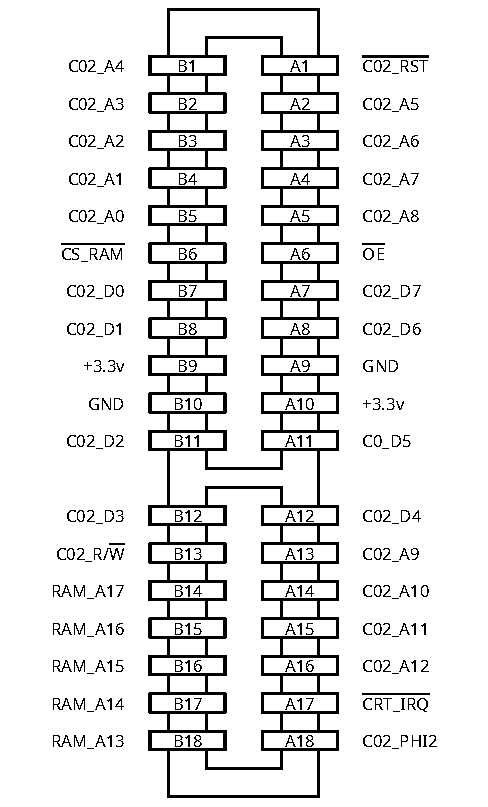
\includegraphics[scale=0.65]{images/f256_port_expansion.pdf}
    \end{center}
    \caption{Expansion Port}
    \label{fig:port_expansion}
\end{figure}

\begin{figure}[ht]
    \begin{center}
        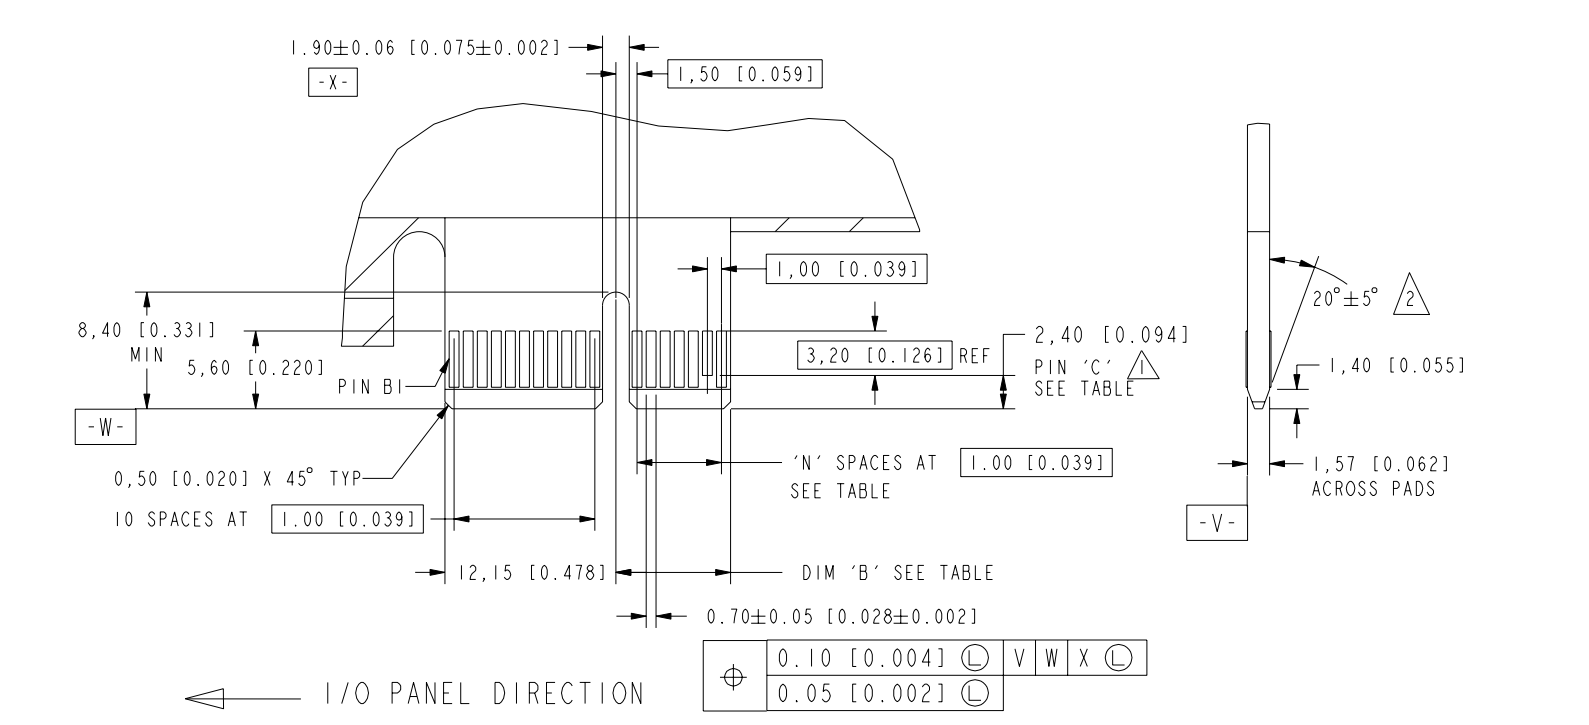
\includegraphics[width=6in]{images/pci.png}
    \end{center}
    \caption{Expansion Port Physical Size}
    \label{fig:port_expan_size}
\end{figure}

% \begin{table}[ht]
%     \begin{center}
%         \begin{tabular}{|c||l|c|c||l|}\cline{1-2}\cline{4-5}
%             B1 & C02\_ADDR4 & \hspace{2em} & A1 & /RST\_IN \\\cline{1-2}\cline{4-5}
%             B2 & C02\_ADDR3 & & A2 & C02\_ADDR5 \\\cline{1-2}\cline{4-5}
%             B3 & C02\_ADDR2 & & A3 & C02\_ADDR6 \\\cline{1-2}\cline{4-5}
%             B4 & C02\_ADDR1 & & A4 & C02\_ADDR7 \\\cline{1-2}\cline{4-5}
%             B5 & C02\_ADDR0 & & A5 & C02\_ADDR8 \\\cline{1-2}\cline{4-5}
%             B6 & /CS\_RAM & & A6 & /OE \\\cline{1-2}\cline{4-5}
%             B7 & C02\_D0 & & A7 & C02\_D7 \\\cline{1-2}\cline{4-5}
%             B8 & C02\_D1 & & A8 & C02\_D6 \\\cline{1-2}\cline{4-5}
%             B9 & +3.3V & & A9 & GND \\\cline{1-2}\cline{4-5}
%             B10 & GND & & A10 & +3.3V \\\cline{1-2}\cline{4-5}
%             B11 & C02\_D2 & & A11 & C02\_D5 \\\cline{1-2}\cline{4-5}
%             B12 & C02\_D3 & & A12 & C02\_D4 \\\cline{1-2}\cline{4-5}
%             B13 & R/W & & A13 & C02\_ADDR9 \\\cline{1-2}\cline{4-5}
%             B14 & RAM\_ADDR17 & & A14 & C02\_ADDR10 \\\cline{1-2}\cline{4-5}
%             B15 & RAM\_ADDR16 & & A15 & C02\_ADDR11 \\\cline{1-2}\cline{4-5}
%             B16 & RAM\_ADDR15 & & A16 & C02\_ADDR12 \\\cline{1-2}\cline{4-5}
%             B17 & RAM\_ADDR14 & & A17 & /CRT\_IRQ \\\cline{1-2}\cline{4-5}
%             B18 & RAM\_ADDR13 & & A18 & C02\_PHI2 \\\cline{1-2}\cline{4-5}
%         \end{tabular}
%     \end{center}
%     \caption{Expansion Connector Pinout}
%     \label{tab:expansion}
% \end{table}
\chapter{I/O Connectors and Jumpers}

\section*{Connectors}

The \jr\ has several connectors on its board for I/O devices beyond the standard connections on the back. Some of these connectors are the only way to access that particular I/O device, but some are auxiliary connectors that provide alternate forms of access. All are IDC header pins. The diagrams that follow show the pin assignments for these connectors. In these diagrams, the views are top-down onto the board, with the board arranged so that the main connectors are towards the top and the power connector is towards the bottom.

\subsection*{Game Connectors}

There are two connectors for game controllers. There are two connectors for Atari style joysticks (figure~\ref{fig:port_joy}). And two for NES or Super NES gamepads (figure~\ref{fig:port_nes}).

For the Atari style joysticks, an adapter cable will be needed to convert from IDC to the standard DB-9 connector. There are two key differences between the \jr\ and Atari or Commodore devices: first, the \jr\ provides 3.3 volts instead of 5 volts, and second there are no paddle inputs supported on the \jr.

For the NES and SNES style gamepads, an adapter box will be needed to provide the correct interfacing for a controller. This adapter should be available from Foenix Retro Systems in the near future (at the time of writing this manual).

\begin{figure}[ht]
    \begin{center}
        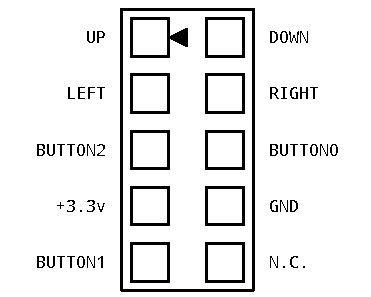
\includegraphics[scale=0.65]{images/f256_port_joystick.pdf}
    \end{center}
    \caption{Joystick Port Pinouts}
    \label{fig:port_joy}
\end{figure}

\begin{figure}[ht]
    \begin{center}
        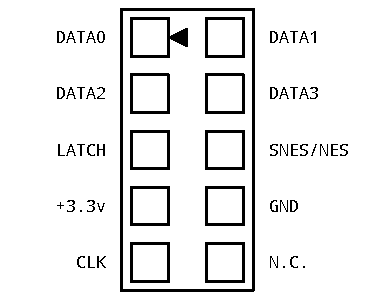
\includegraphics[scale=0.65]{images/f256_port_nes.pdf}
    \end{center}
    \caption{NES/SNES Gamepad Port Pinouts}
    \label{fig:port_nes}
\end{figure}

\subsection*{PS/2 Port}

An internal connector is included for the PS/2 mouse and keyboard port (figure~\ref{fig:port_ps2}). This connector just provides an alternate way of accessing the PS/2 signals. It could be useful in building an integrated case for the \jr\ that includes a PS/2 keyboard.

\begin{figure}[ht]
    \begin{center}
        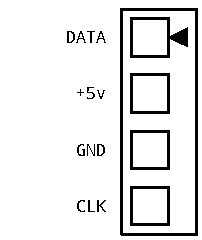
\includegraphics[scale=0.65]{images/f256_port_ps2.pdf}
    \end{center}
    \caption{Auxiliary PS/2 Pinouts}
    \label{fig:port_ps2}
\end{figure}

\subsection*{UART}

This connector provides access to the serial in and out signals for the \jr's UART (figure~\ref{fig:port_uart}). The TxD and RxD signals are compatible with standard $\pm 12$ volt RS-232 signals. The signals on this connector can be brought out to a DB-9 connector to provide a standard 3 wire RS-232 serial port.

\begin{figure}[ht]
    \begin{center}
        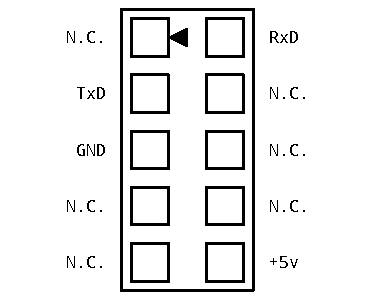
\includegraphics[scale=0.65]{images/f256_port_uart.pdf}
    \end{center}
    \caption{UART Pinouts}
    \label{fig:port_uart}
\end{figure}

An ESP32 Feather board can be installed on the \jr\ to provide access to Wi-Fi, but using this board will take over the supplied UART. Therefore, the \jr\ can provide either an RS-232 serial port or access to Wi-Fi, but not both at the same time. A jumper on the board selects which is active.

\subsection*{USB Debug Port}

While there is a USB Mini-B connector (figure:~\ref{fig:port_usb}) on the port to access the USB debug interface, there is an IDC header connector on the board to provide access to this for the case USB connector, if desired. This is not compatible with all USB case connectors, as many of them are dual connectors and require pins for two USB ports. It should be compatible with cases with single connectors or with panel mounted USB cables.

\begin{figure}[ht]
    \begin{center}
        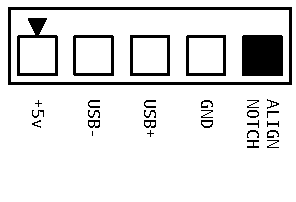
\includegraphics[scale=0.65]{images/f256_port_usb.pdf}
    \end{center}
    \caption{USB Debug Pinouts}
    \label{fig:port_usb}
\end{figure}

\subsection*{Case Connectors}

There are two connectors for the usual PC case connections. There is one for the headphone jack (figure:~\ref{fig:port_audio}), and one for the various buttons, LEDs, and case speaker (figure:~\ref{fig:port_case}): power, reset, hard drive/SD card activity. Note that while the speaker and buttons are not polarized, the power LED and hard-drive activity LED are and must be wired in the correct orientation.

\begin{figure}[ht]
    \begin{center}
        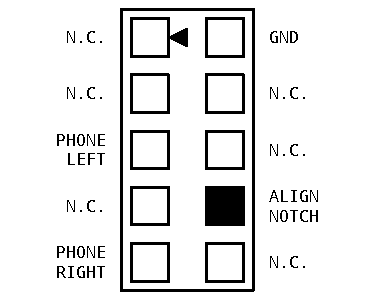
\includegraphics[scale=0.65]{images/f256_port_audio.pdf}
    \end{center}
    \caption{Case Audio Pinouts}
    \label{fig:port_audio}
\end{figure}

\begin{figure}[ht]
    \begin{center}
        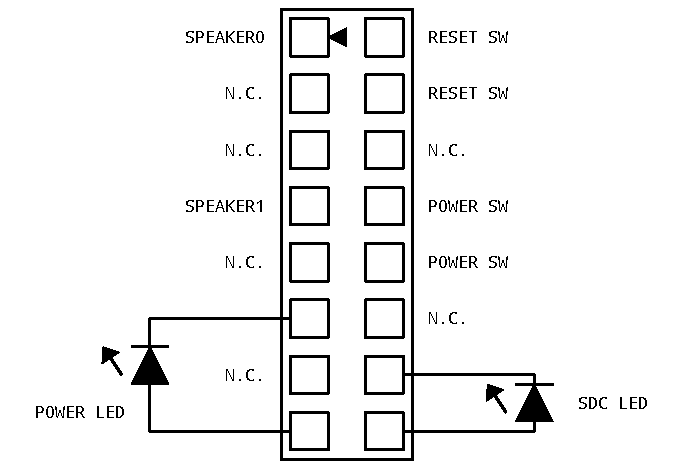
\includegraphics[scale=0.65]{images/f256_port_case.pdf}
    \end{center}
    \caption{Case Button and LED Pinouts}
    \label{fig:port_case}
\end{figure}

Not shown is a small secondary connector for an SPST switch for power (the connector is located at the front-right corner of the \fjr\ RevB board). This connector provides an alternative to the usual case power push button. The two buttons cannot be used together. Either the case push button shown in \ref{fig:port_case} is used, or the other SPST switch is used, but not both.

\section*{Jumpers}

There are several IDC header pins with jumpers to configure various options on the \jr. All the jumper headers are three pin headers, where the center pin is the common. The header is used to select the appropriate routing of a signal or voltage level. So the jumper is always used to connect the center common pin to either the left or right pins (or the top or bottom, depending on the orientation of the header).

\subsection*{SID Jumpers}

The SID chips have two sets of jumpers each. The first pair are the voltage selection jumpers. They can be used to select the appropriate voltage for the SID chip: 12 volts for the original 6581, and 9 volts for the later 8580 (see figure~\ref{fig:jmp_sid_voltage}). If you are using a modern replacement, check the instructions as to which voltage to use: some replacements work with either voltage.

\begin{figure}[ht]
    \begin{center}
        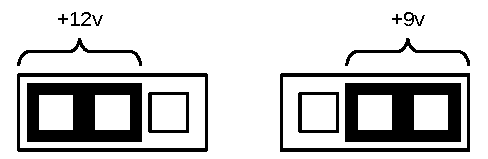
\includegraphics[scale=0.65]{images/jumper_voltage.pdf}
    \end{center}
    \caption{SID Voltage Jumper}
    \label{fig:jmp_sid_voltage}
\end{figure}

The second pair of SID jumpers are the channel selectors (see figure~\ref{fig:jmp_sid_channel}). These jumpers select the source of the left and right channels for the CODEC. With each one, you can select either the right or the left SID as an input to the CODEC for that stereo channel. If a \fjr\ is using both SIDs, the left channel should select the left SID, and the right channel select the right SID. But if only a single SID is used, both channels can be set to that SID. For instance, if the SID is in the left socket, both left and right channels can select the left SID as the source to get a balanced monaural sound.

\begin{figure}[ht]
    \begin{center}
        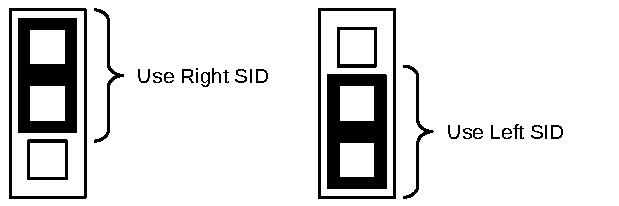
\includegraphics[scale=0.65]{images/jumper_channel.pdf}
    \end{center}
    \caption{SID Stereo Channel Source Jumper}
    \label{fig:jmp_sid_channel}
\end{figure}

\subsection*{Boot Source}

There is a jumper to select boot source (see figure~\ref{fig:jmp_boot}). With the jumper in the left position, the \fjr\ will boot off the flash, using the last 8KB bank of flash memory as the last 8KB of CPU address space. With the jumper in the right position, the \fjr\ will boot using RAM. See page~\ref{pg:mmu_boot_config} for a more complete description of boot sources.

\begin{figure}[ht]
    \begin{center}
        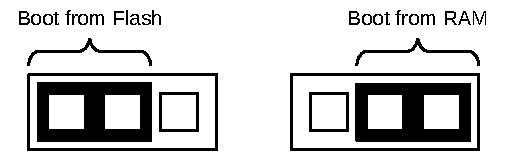
\includegraphics[scale=0.65]{images/jumper_boot.pdf}
    \end{center}
    \caption{Boot Source Jumper}
    \label{fig:jmp_boot}
\end{figure}

\subsection*{UART Configuration}

There are two headers for selecting how the UART is used---selecting between the serial port or the ESP32 Wi-Fi module (see figure~\ref{fig:jmp_uart}). One jumper controls the routing of the TxD line, while the other controls the routing of the RxD line. With the jumper positioned across the ``back'' pair of pins, the signal is routed to the Wi-Fi module. With the jumper positioned across the ``front'' pair of pins, the signal is routed to the DB-9 port connected to the UART connector. Note that both the TxD and RxD jumpers should be in the same relative position so that they both use the same device.

\begin{figure}[ht]
    \begin{center}
        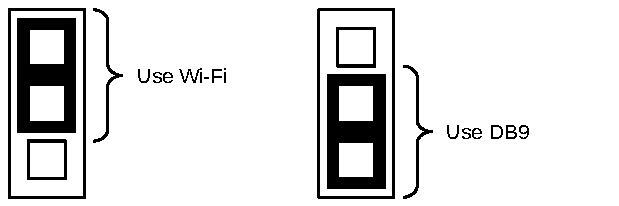
\includegraphics[scale=0.65]{images/jumper_uart.pdf}
    \end{center}
    \caption{UART Device Jumpers}
    \label{fig:jmp_uart}
\end{figure}
\chapter{Memory Maps}

\begin{table}[h]
    \begin{center}
        \begin{tabular}{|c|l|} \hline
            Address & Purpose \\ \hline\hline
            \verb+0x00000+ & \multirow{2}{*}{System RAM for programs, data, and graphics (256 KB)} \\ \cline{1-1}
            \verb+0x3FFFF+ & \\ \hline
            \verb+0x40000+ & \multirow{2}{*}{Reserved (256 KB)} \\ \cline{1-1}
            \verb+0x7FFFF+ & \\ \hline
            \verb+0x80000+ & \multirow{2}{*}{Flash memory (512 KB)} \\ \cline{1-1}
            \verb+0xFFFFF+ & \\ \hline
        \end{tabular}
    \end{center}
    \caption{System Memory Map for the \jr}
    \label{tab:sys_mem_map}
\end{table}

\begin{table}[h]
    \begin{center}
        \begin{tabular}{|c|c|l|} \hline
            Bank & Purpose \\ \hline\hline
            \multirow{10}{*}{0} & \verb+0x0000+ & MMU Memory Control Register \\ \cline{2-3}
            & \verb+0x0001+ & MMU I/O Control Register \\ \cline{2-3}
            & \verb+0x0002+ & \multirow{2}{*}{RAM or Flash} \\ \cline{2-2}
            & \verb+0x0007+ & \\ \cline{2-3}
            & \verb+0x0008+ & \multirow{2}{*}{RAM, Flash, or MMU LUT Registers} \\ \cline{2-2}
            & \verb+0x000F+ & \\ \cline{2-3}
            & \verb+0x0010+ & \multirow{2}{*}{65C02 Page Zero} \\ \cline{2-2}
            & \verb+0x00FF+ & \\ \cline{2-3}
            & \verb+0x0100+ & \multirow{2}{*}{65C02 Stack} \\ \cline{2-2}
            & \verb+0x01FF+ & \\ \cline{2-3}
            & \verb+0x0200+ & \multirow{2}{*}{RAM or Flash} \\ \cline{2-2}
            & \verb+0x1FFF+ & \\ \hline
            \multirow{2}{*}{1} & \verb+0x2000+ & \multirow{2}{*}{RAM or Flash} \\ \cline{2-2}
            & \verb+0x3FFF+ & \\ \hline
            \multirow{2}{*}{2} & \verb+0x4000+ & \multirow{2}{*}{RAM or Flash} \\ \cline{2-2}
            & \verb+0x5FFF+ & \\ \hline
            \multirow{2}{*}{3} & \verb+0x6000+ & \multirow{2}{*}{RAM or Flash} \\ \cline{2-2}
            & \verb+0x7FFF+ & \\ \hline
            \multirow{2}{*}{4} & \verb+0x8000+ & \multirow{2}{*}{RAM or Flash} \\ \cline{2-2}
            & \verb+0x9FFF+ & \\ \hline
            \multirow{2}{*}{5} & \verb+0xA000+ & \multirow{2}{*}{RAM or Flash} \\ \cline{2-2}
            & \verb+0xBFFF+ & \\ \hline
            \multirow{2}{*}{6} & \verb+0xC000+ & \multirow{2}{*}{RAM, Flash, I/O, Text mode character, or color data} \\ \cline{2-2}
            & \verb+0xDFFF+ & \\ \hline
            \multirow{8}{*}{7} & \verb+0xE000+ & \multirow{2}{*}{RAM or Flash} \\ \cline{2-2}
            & \verb+0xFFFA+ & \\ \cline{2-3}
            & \verb+0xFFFA+ & \multirow{2}{*}{65C02 NMI Vector} \\ \cline{2-2}
            &\verb+0xFFFB+ & \\ \cline{2-3}
            &\verb+0xFFFC+ & \multirow{2}{*}{65C02 Reset Vector} \\ \cline{2-2}
            &\verb+0xFFFD+ & \\ \cline{2-3}
            &\verb+0xFFFE+ & \multirow{2}{*}{65C02 IRQ Vector} \\ \cline{2-2}
            &\verb+0xFFFF+ & \\ \hline
        \end{tabular}
    \end{center}
    \caption{CPU Memory Map for the \jr}
    \label{tab:cpu_mem_map}
\end{table}

\begin{table}
    \begin{center}
        \begin{tabular}{|c|c|l|} \hline
            Start & End & Purpose \\ \hline \hline
            \verb+0xC000+ & \verb+0xC3FF+ & Gamma Table Blue \\ \hline
            \verb+0xC400+ & \verb+0xC7FF+ & Gamma Table Green \\ \hline
            \verb+0xC800+ & \verb+0xCBFF+ & Gamma Table Red \\ \hline
            \verb+0xCC00+ & \verb+0xCFFF+ & Reserved \\ \hline
            \verb+0xD000+ & \verb+0xD0FF+ & VICKY Master Control Registers \\ \hline
            \verb+0xD100+ & \verb+0xD1FF+ & VICKY Bitmap Control Registers \\ \hline
            \verb+0xD200+ & \verb+0xD2FF+ & VICKY Tile Control Registers \\ \hline
            \verb+0xD300+ & \verb+0xD3FF+ & Reserved \\ \hline
            \verb+0xD400+ & \verb+0xD4FF+ & SID Left \\ \hline
            \verb+0xD500+ & \verb+0xD4FF+ & SID Right \\ \hline
            \verb+0xD600+ & \verb+0xD60F+ & PSG Left \\ \hline
            \verb+0xD610+ & \verb+0xD61F+ & PSG Right \\ \hline
            \verb+0xD620+ & \verb+0xD62F+ & CODEC \\ \hline
            \verb+0xD630+ & \verb+0xD63F+ & UART \\ \hline
            \verb+0xD640+ & \verb+0xD64F+ & PS/2 Interface \\ \hline
            \verb+0xD650+ & \verb+0xD65F+ & Timers \\ \hline
            \verb+0xD660+ & \verb+0xD66F+ & Interrupt Controller \\ \hline
            \verb+0xD670+ & \verb+0xD67F+ & DIP Switch \\ \hline
            \verb+0xD680+ & \verb+0xD68F+ & IEC Controller \\ \hline
            \verb+0xD690+ & \verb+0xD69F+ & Real Time Clock \\ \hline
            \verb+0xD6A0+ & \verb+0xD6AF+ & System Control Registers \\ \hline
            \verb+0xD6B0+ & \verb+0xD7FF+ & Reserved \\ \hline
            \verb+0xD800+ & \verb+0xD83F+ & Text Foreground Color LUT \\ \hline
            \verb+0xD840+ & \verb+0xD87F+ & Text Background Color LUT \\ \hline
            \verb+0xD880+ & \verb+0xD8FF+ & Reserved \\ \hline
            \verb+0xD900+ & \verb+0xDAFF+ & VICKY Sprite Control Registers \\ \hline
            \verb+0xDB00+ & \verb+0xDBFF+ & Reserved \\ \hline
            \verb+0xDC00+ & \verb+0xDCFF+ & 65C22 VIA Control Registers \\ \hline
            \verb+0xDD00+ & \verb+0xDDFF+ & SD Card Controller \\ \hline
        \end{tabular}
        \caption{I/O Page 0 Addresses}
        \label{tab:io_page_0}
    \end{center}
\end{table}


\begin{table}[h]
    \begin{center}
        \begin{tabular}{|c|c|l|} \hline
            Start & End & Purpose \\ \hline\hline
            \verb+0xC000+ & \verb+0xC7FF+ & Text Mode Font Memory \\ \hline
            \verb+0xC800+ & \verb+0xCFFF+ & Reserved \\ \hline
            \verb+0xD000+ & \verb+0xD3FF+ & Graphics Color LUT 0 \\ \hline
            \verb+0xD400+ & \verb+0xD7FF+ & Graphics Color LUT 1 \\ \hline
            \verb+0xD800+ & \verb+0xDBFF+ & Graphics Color LUT 2 \\ \hline
            \verb+0xDC00+ & \verb+0xDFFF+ & Graphics Color LUT 3 \\ \hline
        \end{tabular}
    \end{center}
    \caption{Memory Map for I/O Page 1}
    \label{tab:map_io_1}
\end{table}

% \chapter{The TinyCore 65c02 MicroKernel F256(K) Edition}
\label{chp:kernel}

\begin{leftbar}
  NOTE: This chapter was written by Jessie Oberreuter to describe her MicroKernel for the F256 family and is covered under her project's copyright. It is included here by her kind permission. The link to get the API files and sample code for the kernel is listed below and in the References chapter at the end of the manual.
\end{leftbar}
  
The TinyCore 6502 MicroKernel for the Foenix F256/F256K line of computers is a powerful alternative to the typical BIOS style kernels that come with most 8-bit computers.  This kernel offers the following features:

\begin{itemize}
    \item An event-based programming model for real-time games and VMs.
    \item A network stack supporting multiple concurrent TCP and UDP sockets.
    \item Drivers for optional ESP8266 based wifi modules.
    \item Drivers for IEC drives.
    \item Drivers for Fat32 formatted SD Cards.
    \item Support for PS2 keyboards, Foenix keyboards, and CBM keyboards
    \item Support for PS2 scroll mice.
    \item Preemptive kernel multi-tasking (no need to yield). 
\end{itemize}

The TinyCore 65c02 MicroKernel is Copyright 2022 Jessie Oberreuter
The Fat32 library is Copyright 2020 Frank van den Hoef and Michael Steil  

There's a lot of love in here; I hope you will enjoy using it as much as I have enjoyed writing it! --- Gadget.

\section*{Setup and Installation}

\subsection*{Getting the Kernel}
Kernel binaries may be obtained from either of the following repos: 

\begin{itemize}
    \item  https://github.com/ghackwrench/F256\_Jr\_Kernel\_DOS
    \item  https://github.com/paulscottrobson/superbasic
\end{itemize}

The `ghackwrench' repo contains the latest release.  The `paulscottrobson' repo contains the latest version verified to work with SuperBASIC.

\subsection*{Flashing the Kernel}
The kernel consists of four 8k blocks which must be flashed into the last four blocks of the F256.  Using the F256 Programmer Tool (Windows), the kernel needs to be flashed into Flash Blocks 0x3C--0x3F.  Alternately, the SuperBASIC repo contains a script which uses a python based loader to install SuperBASIC along with the Kernel.

\subsection*{DIP Switches}
The kernel assigns the DIP switches as follows:

\begin{enumerate}
\item Enable boot-from-RAM
\item Reserved (potentially for SNES gamepad support)
\item Enable SLIP based networking
\item Feather board installed ({\it e.g.} Huzzah 8266 WiFi)
\item SIDs are installed
\item F256: CBM keyboard installed; F256k: audio expansion installed.
\item ON: 640x480, OFF: 640x400 ({\em not yet implemented})
\item Enable gamma color correction
\end{enumerate}

When boot-from-RAM is enabled, the kernel will search the first 48k of RAM for pre-loaded programs before starting the first program on the expansion cartridge or the first program in flash.

\subsection*{Support Software}
\begin{itemize}
    \item The superbasic repo contains a powerful BASIC programming language which has been ported to run on the MicroKernel.
    \item The Kernel\_DOS repo includes a simple DOS CLI which demonstrates most kernel functions.
    \item The Kernel\_DOS repo also contains library and config files for compiling C programs with cc65 for use with the MicroKernel.
\end{itemize}

\section*{Memory Model}
The F256 series machines minimally reserve addresses 0x00 and 0x01 for memory and I/O control.  Programs may optionally enable additional hardware registers from 0x08--0x0f.

The MicroKernel uses 16 bytes of the Zero page, from 0xf0--0xff, for the \verb+kernel.args+ struct.  Kernel calls do not expect their arguments to come in registers.  Instead, all kernel arguments are passed by writing them to variables in \verb+kernel.args+.  The \verb+A+ register is used by all kernel calls.  The \verb+X+ and \verb+Y+ registers, however, are always preserved.  All kernel calls clear the carry on success and set the carry on failure.  A few calls return a stream id in \verb+A+ as a convenience, but most of the time, \verb+A+ should just be considered undefined upon return from the kernel.

Outside of the above, user programs are free to use all addresses up to 0xC000 as they wish.

0xC000--0xDFFF is the I/O window.  The I/O window can be disabled to reveal RAM underneath, but programs should refrain from doing so, as this RAM is used by the kernel.  Programs are generally free to use the hardware as they see fit, but note that, by default, the kernel takes ownership of the PS2 ports, the frame interrupt, and the RTC interrupt, and will take ownership of the serial port if either the SLIP or Feather DIP switches are set.

0xE000--0xFFFF contains the kernel itself.  The kernel is considerably larger than 8kB, but it uses the F256 MMU hardware to keep its footprint in the user's memory map to a relative minimum.

The F256 machines support four concurrent memory maps.  The kernel reserves map zero for itself, and map one for the Fat32 drivers; user programs are run from map three.  Map two is potentially reserved for a hypervisor. 

The kernel uses only two 8k blocks of RAM: block 6 (nominally at 0xC000), and block 7 (nominally at 0xE000).  Everything else is free for use by user software.

\section*{Startup}
On power-on or reset, the kernel initializes the hardware according to the DIP switches and then searches various memory regions for the first program to run.  If DIP1 is on, it first checks RAM blocks 1--5 for a pre-loaded binary.  After that, it searches the expansion RAM/ROM blocks, and, finally, the on-board flash blocks. The first block found with a valid header will be mapped into MMU 3 and started.  The header must appear at the very start of the block and contains the following fields:

\begin{verbatim}
Byte  0    signature: 0xF2
Byte  1    signature: 0x56
Byte  2    the size of program in 8k blocks
Byte  3    the starting slot of the program (ie where to map it)
Bytes 4-5  the start address of the program
Bytes 6-9  reserved
Bytes 10-  the zero-terminated name of the program.
\end{verbatim}

\section*{Programming}
With a 65c02 installed, the F256 machines can generally be treated as simple 6502 machines.  Programs have full access to the RAM from 0x0000--0xBFFF, and full access to I/O from 0xC000--0xDFFF.  More adventurous programs can enable the MMU registers and bank additional memory into any 8k slot below 0xC000.  Really adventurous programs are free to disable interrupts, map out the kernel, and take complete control over the machine.  Programs wishing to use the kernel, however, should be sure to keep interrupts enabled as much as possible, call \verb+NextEvent+ often enough that the kernel doesn't run out of event objects, and refrain from trashing MMU LUT0, MMU LUT1, and the RAM between 0xC000 and 0xFFFF.

The kernel interfaces are described below using their symbolic names.  The actual values and addresses must be obtained by including either \verb+api.asm+ or \verb+api.h+ in your project.

\section*{Events}
The F256 machines were designed for games, and the 6502 TinyCore MicroKernel was designed to match.

Games generally run in a simple loop:

\begin{enumerate}
    \item Update the screen
    \item Read the controls
    \item Update the game state
    \item Goto 1
\end{enumerate}

The kernel supports this mode of operation by replacing step 2 above (read the controls) with a generic kernel call: \verb+NextEvent+.  \verb+NextEvent+ gets the next I/O event from the kernel's queue and copies it into a user provided buffer.  

\subsection*{Setup}
Events are 8-byte packets.  Each packet contains four common bytes, and up to four event-specific bytes.  The user's buffer for these bytes may be placed anywhere, but since they are accessed frequently, the zero page is a good place.

Before a program can receive events, it must tell the kernel where events should be copied.  It does this by writing the address of an 8-byte buffer into the kernel's \verb+arg+ block:

\begin{verbatim}
    .section zp
event   .dstruct	 kernel.event.event_t
    .send

    .section code

init_events

    lda     \#<event
    sta     kernel.args.events+0
    lda     \#>event
    sta     kernel.args.events+1
    rts
\end{verbatim}

\subsection*{Handling}
For games, and other real-time applications, a program will typically contain a single "handle\_events" routine:

\begin{verbatim}
handle_events

    ; Peek at the queue to see if anything is pending
    lda		kernel.events.pending  ; Negated count
    bpl		_done

    ; Get the next event.
    jsr		kernel.NextEvent
    bcs		_done

    ; Handle the event
    jsr		_dispatch
            
    ; Continue until the queue is drained.
    bra		handle_events
            
_done

    rts

_dispatch

    ; Get the event's type
    lda		event.type
    					
    ; Call the appropriate handler

    cmp		#kernel.event.key.PRESSED
    beq		_key_pressed

    cmp		#kernel.event.mouse.DELTA
    beq		_mouse_moved
			
    ...
    rts     ; Anything not handled can be ignored.
\end{verbatim}

Other types of programs may eschew the use of a single central event handler, and instead work the queue only when waiting for events, and then only to handle the event types expected for the operation.  The F256 cc65 kernel library does just this: when waiting for keypresses, it only handles key events; when waiting for data from a file, it only handles file.DATA/EOF/ERROR events and ignores all others.  This approach is considerably simpler but also considerably less powerful.

\subsection*{Event types}
Events belong to one of two categories: {\em Solicited Events} and {\em Unsolicited Events}.

{\em Solicited Events} are events which are generated in response to I/O requests ({\it e.g.} file Open/Read/Close calls).  {\em Unsolicited Events} are generated by external devices such as keyboards, joysticks, and mice.  {\em Unsolicited Events} are also generated whenever packets are received from the network.

\subsubsection*{Solicited Events}
The {\em solicited events} are described in the {\em Kernel Calls} section below.  The documentation for each kernel call that queues an event includes a description of the possible events.

\subsubsection*{Unsolicited Events}
\begin{verbatim}
event.key.PRESSED
event.key.RELEASED
\end{verbatim}

These events occur whenever a key is pressed or released:

\begin{itemize}
    \item \verb+event.key.keyboard+ contains the id of the keyboard.
    \item \verb+event.key.raw+ contains the raw key-code (see \verb+kernel/keys.asm+).
    \item \verb+event.key.flags+ is negative if this is a meta (non-ascii) key.
    \item \verb+event.key.ascii+ contains the ascii interpretation if available.
\end{itemize}

\begin{verbatim}
event.mouse.DELTA
\end{verbatim}

This event is generated every time the mouse is moved or a button changes state.

\begin{itemize}
\item \verb+event.mouse.delta.x+ contains the x delta.
\item \verb+event.mouse.delta.y+ contains the y delta.
\item \verb+event.mouse.delta.z+ contains the z (scroll) delta.
\item \verb+event.mouse.delta.buttons+ contains the button bits.
\end{itemize}

The buttons are encoded as follows:

\begin{itemize}
\item Bit 0 (1) is the inner-most button
\item Bit 1 (2) is the middle button
\item Bit 2 (4) is the outer-most button
\end{itemize}

The bits are set when the button is pressed and cleared when the button is released.

To change the ``handedness'' of the mouse, simply place it in whichever hand you prefer, and double-click!  

\begin{verbatim}
event.mouse.CLICKS
\end{verbatim}

This event reports mouse click (press-and-release) events.  Whenever a mouse button is pressed, the kernel starts a 500ms timer and counts the number of times each button is both pressed and released.  At the end of the 500ms, the counts are reported:

\begin{itemize}
\item \verb+event.mouse.clicks.inner+ contains the count of inner clicks.
\item \verb+event.mouse.clicks.middle+ contains the count of middle clicks.
\item \verb+event.mouse.clicks.outer+ contains the count of outer clicks.
\end{itemize}

A report of all zeros indicates that a press-and-hold is in progress; programs should consult the most recent event.\verb+mouse.DELTA+ event to determine which button(s) are being held. 

\begin{verbatim}
event.JOYSTICK+
\end{verbatim}

This event returns the state of the ``buttons'' for each of the two joysticks whenever either's state changes:

\begin{itemize}
\item \verb+event.joystick.joy0+ contains the bits for Joystick 0.
\item \verb+event.joystick.joy1+ contains the bits for Joystick 1.
\end{itemize}

The bits are set when the associated switch is pressed, and clear when released.

\begin{verbatim}
event.TCP
event.UDP
event.ICMP
\end{verbatim}

These events are generated whenever a network packet of the given type is received.  For TCP and UDP packets, a program can use the \verb+kernel.Net.Match+ call to see if the packet matches an open socket.  Non-matching UDP packets can be ignored; network aware programs should respond to unmatched TCP packets by calling \verb+kernel.Net.TCP.Reject+. TCP and UDP payloads may be read by calling \verb+kernel.Net.TCP.Recv+ and \verb+kernel.Net.UDP.Recv+ respectively.  For ICMP packets, programs can get the raw data by calling \verb+kernel.ReadData+.   

\begin{verbatim}
event.clock.TICK
\end{verbatim}

This event is generated every second for general time reference.


\section*{Kernel Calls}

\subsection*{Generic Calls}

\subsubsection*{NextEvent}
Copies the next event from the kernel's event queue into a user provided event buffer.

\paragraph{Input}
\begin{itemize}
\item \verb+kernel.args.events+ points to an 8-byte buffer.  
\end{itemize}

\paragraph{Output}
\begin{itemize}
\item Carry cleared on success.
\item Carry set if no events are pending.
\end{itemize}

\paragraph{Effect}
\begin{itemize}
\item If there is an event in the queue, it is copied into the provided buffer.
\end{itemize}

\paragraph{Notes}
\begin{itemize}
\item \verb+kernel.args.events+ is a reserved field in the argument block; nothing else uses this space, so you need only initialize this pointer once on startup.
\item \verb+kernel.args.pending+ contains the count of pending events (negated for ease of testing with BIT).  You can save considerable CPU time by testing \verb+kernel.args.pending+ and only calling \verb+NextEvent+ if it is non-zero.
\item The kernel reports almost everything through events.  Consider keeping the event buffer in the zeropage for efficient access.
\end{itemize}


\subsection*{ReadData}
Copies data from the kernel buffer associated with the current event into the user's address space.

\paragraph{Input}
\begin{itemize}
\item \verb+kernel.args.buf+ points to a user buffer.
\item \verb+kernel.args.buflen+ contains the number of bytes to copy (0=256).
\end{itemize}

\paragraph{Output}
\begin{itemize}
\item Carry cleared.
\end{itemize}

\paragraph{Effect}
\begin{itemize}
\item The contents of the current event's primary buffer are copied into the provided user buffer.
\item If the event doesn't contain a buffer, zeros are copied.
\end{itemize}

\subsection*{ReadExt}
Copies extended data from the kernel buffer associated with the current event into the user's address space.

\paragraph{Input}
\begin{itemize} 
\item \verb+kernel.args.buf+ points to a user buffer.
\item \verb+kernel.args.buflen+ contains the number of bytes to copy (0=256).
\end{itemize}

\paragraph{Output}
\begin{itemize}
\item Carry cleared.
\end{itemize}

\paragraph{Effect}
\begin{itemize}
\item The contents of the current event's primary buffer are copied into the provided user buffer.
\item If the event doesn't contain an extended data buffer, zeros are copied.
\end{itemize}

\paragraph{Notes}
\begin{itemize}
\item Events with extended data are relatively rare.  Typical examples include file meta-information and bytes 256...511 of a 512 byte raw-sector read. 
\end{itemize}


\subsection*{Yield}
Yields the CPU to the kernel.  This is typically used to expedite the processing of network packets.  It is never required.

\paragraph{Input}
\begin{itemize}
\item none
\end{itemize}

\paragraph{Output}
\begin{itemize}
\item none
\end{itemize}

\paragraph{Effects}
\begin{itemize}
\item none
\end{itemize}


\subsection*{RunBlock}
Transfers execution to the program found in the given memory block.

\paragraph{Input}
\begin{itemize}
\item \verb+kernel.args.run.block_id+ contains the number of the block to execute.
\end{itemize}

\paragraph{Output}
\begin{itemize}
\item On success, the call doesn't return.
\item Carry set on error (block doesn't contain a program).
\end{itemize}


\subsection*{RunNamed}
Transfers execution to the first program found with the given name.

\paragraph{Input}
\begin{itemize}
\item \verb+kernel.args.buf+ points to a buffer containing the name of the program to run.
\item \verb+kernel.args.buflen+ contains the length of the name. 
\end{itemize}

\paragraph{Output}
\begin{itemize}
\item On success, the call doesn't return.
\item Carry set on error (a program with the provided name was not found).
\end{itemize}

\paragraph{Notes}
\begin{itemize}
\item The name match is case-insensitive.
\end{itemize}


\section*{FileSystem Calls}

\subsection*{FileSystem.MkFS}
Creates a new filesystem on the given device.

\paragraph{Input}
\begin{itemize}
\item \verb+kernel.args.fs.mkfs.drive+ contains the device number (0 = SD, 1 = IEC \#8, 2 = IEC \#9)
\item \verb+kernel.args.fs.mkfs.label+ points to a buffer containing the new drive label.
\item \verb+kernel.args.fs.mkfs.label_len+ contains the length of the label buffer (0=0).
\item \verb+kernel.args.fs.mkfs.cookie+ contains a user-provided cookie for matching against completion events.
\end{itemize}

\paragraph{Output}
\begin{itemize}
\item Carry cleared on success.
\item Carry set on error (device doesn't exist, kernel is out of streams).
\end{itemize}

\paragraph{Events}
\begin{itemize}
\item The kernel will queue an \verb+event.fs.CREATED+ event on success.
\item The kernel will queue an \verb+event.fs.ERROR+ event on failure.
\end{itemize}

\paragraph{Notes}
\begin{itemize}
\item This is presently an atomic, blocking call on both IEC and Fat32, and it can take a {\em long} time to complete.  While running, your program will not be able to work the event queue, so pretty much the whole system will grind to a halt.  Until this changes, it's best if interactive programs and operating systems avoid this call.  
\end{itemize}

\section*{File Calls}

\subsection*{Open}
Opens a file for read, append, or create/overwrite.  The file should not be concurrently opened in another stream.

\paragraph{Input}
\begin{itemize}
\item \verb+kernel.args.file.open.drive+ contains the drive ID (0 = SD card, 1 = IEC \#8, 2 = IEC \#9).
\item \verb+kernel.args.file.open.fname+ points to the name of the file.
\item \verb+kernel.args.file.open.fname_len+ contains the length of the name.
\item \verb+kernel.args.file.open.mode+ contains the access mode (0 = read, 1 = write, 2 = append). 
\item \verb+kernel.args.file.open.cookie+ contains an optional, user provided value which will be returned in subsequent events related to this file.
\end{itemize}

\paragraph{Output}
\begin{itemize}
\item Carry cleared on success, and \verb+A+ contains the stream ID for the file.
\item Carry set if the drive isn't found, or if the kernel lacks sufficient resources to complete the call.
\end{itemize}

\paragraph{Events}
\begin{itemize}
\item On a successful open/create/append, the kernel will queue a \verb+file.OPENED+ event.
\item For read or append, if the file does not exist, the kernel will queue a \verb+file.NOT_FOUND+ event.
\item File events contain the stream id (in \verb+event.file.stream+) and the user supplied cookie (in\\ \verb+event.file.cookie+).
\end{itemize}

\paragraph{Notes}
\begin{itemize}
\item The kernel supports a maximum of 20 concurrently opened files (including directories and rename/delete operations) across all devices.
\item The IEC driver supports a maximum of 8 concurrently opened files (not counting directories and rename/delete operations) per device. 
\item Fat32 preserves case when creating files, and uses case-insensitive matching when opening files.
\item IEC devices vary in their handling of case.  Users will just need to live with this.
\item Unlike other kernel calls, most file operations are blocking.  In the case of IEC, this is due to the fact that an interrupt driven interface was not available at the time of writing (it is now, so IEC can be improved).  In the case of Fat32, the fat32.s package we're using contains its own, blocking SPI stack (which may be replaced in the future).  Fortunately, most operations are fast enough that events won't be dropped.
\item The kernel does not lock files and does not check to see if a file is already in use.  Should you attempt to concurrently open the file in two or more streams, the resulting behavior is entirely up to the device (IEC) or the file-system driver (fat32.s).  The above statement that the file should not be concurrently opened should be treated as a strong warning. 
\item {\em Open for append is not yet implemented}
\end{itemize}


\subsection*{File.Read}
Reads bytes from a file opened for reading.

\paragraph{Input}
\begin{itemize}
\item \verb+kernel.args.file.read.stream+ contains the stream ID of the file (the stream is returned in the \verb+file.OPENED+ event and from the \verb+File.Open+ call itself).
\item \verb+kernel.args.file.read.buflen+ contains the requested number of bytes to read.
\end{itemize}

\paragraph{Output}
\begin{itemize}
\item Carry cleared on success.
\item Carry set on error (file is not opened for reading, file is in the EOF state, the kernel is out of event objects).
\end{itemize}

\paragraph{Events}
\begin{itemize}
\item On a successful read, the kernel will queue an \verb+event.file.DATA+ event (see \verb+ReadData+). \\ \verb+event.file.data.requested+ contains the number of bytes requested;  \verb+event.file.data.read+ contains the number of bytes actually read.
\item On EOF, the kernel will queue an \verb+event.file.EOF+ event.
\item On error, the kernel will queue an \verb+event.file.ERROR+ event.
\item In all cases, the event will also contain the stream id in \verb+event.file.stream+ and the the user's cookie in \verb+event.file.cookie+.
\end{itemize}

\paragraph{Notes}
\begin{itemize}
\item As with POSIX, the kernel may return fewer bytes than requested.  This is not an error, and does not imply that the file has reached EOF (the kernel will queue an \verb+event.file.EOF+ on EOF).  When this happens, the user is expected to simply call \verb+File.Read+ again to get more data.

\item IEC devices don't report file-not-found until a read is attempted.  To work around this issue, when talking to an IEC device, File.Open performs a one-byte read during the open.  This single byte is later returned in the file's first \verb+event.file.DATA+ response (it does not attempt to merge this byte into the next full read).  

\item To reduce the risk of losing events while reading data from IEC devices, IEC read transfers are artificially limited to 64 bytes at a time.  This limit may be lifted once we have interrupt driven IEC transfers.
\end{itemize}

\subsection*{File.Write}
Writes bytes to a file opened for writing.

\paragraph{Input}
\begin{itemize}
\item \verb+kernel.args.file.write.stream+ contains the stream ID of the file (the stream is returned in the \verb+file.OPENED+ event and from the \verb+File.Open+ call itself).
\item \verb+kernel.args.file.write.buf+ points to the buffer to write.
\item \verb+kernel.args.file.write.buflen+ contains the requested number of bytes to write.
\end{itemize}

\paragraph{Output}
\begin{itemize}
\item Carry cleared on success.
\item Carry set on error (file is not opened for writing, the kernel is out of event objects).
\end{itemize}

\paragraph{Events}
\begin{itemize}
\item On a successful write, the kernel will queue an \verb+event.file.WROTE+ event. \\ \verb+event.file.wrote.requested+ contains the number of bytes requested; \\ \verb+event.file.wrote.wrote+ contains the number of bytes actually written.
\item On error, the kernel will queue an \verb+event.file.ERROR+ event.
\item In all cases, the event will also contain the stream id in \verb+event.file.stream+ and the user's cookie in \verb+event.file.cookie+.
\end{itemize}

\paragraph{Notes}
\begin{itemize}
\item As with POSIX, the kernel may write fewer bytes than requested.  This is not an error.  When it happens, the user is expected to simply call \verb+File.Write+ again to write more data.

\item To reduce the risk of losing events while reading data from IEC devices, IEC write transfers are artificially limited to 64 bytes at a time.  This limit may be lifted once we have interrupt driven IEC transfers.
\end{itemize}

\subsection*{File.Seek}
Changes the position of the next read or write within a file.

\paragraph{Input}
\begin{itemize}
\item \verb+kernel.args.file.seek.stream+ contains the stream ID of the file (the stream is returned in the \verb+file.OPENED+ event and from the \verb+File.Open+ call itself).
\item \verb+kernel.args.file.seek.offset+ contains the 32-bit file offset.
\end{itemize}

\paragraph{Output}
\begin{itemize}
\item Carry cleared on success.
\item Carry set on error (the kernel is out of event objects).
\end{itemize}

\paragraph{Events}
\begin{itemize}
\item On a successful write, the kernel will queue an \verb+event.file.SEEK+ event.
\item On error, the kernel will queue an \verb+event.file.ERROR+ event.
\item In all cases, the event will also contain the stream id in \verb+event.file.stream+ and the the user's cookie in \verb+event.file.cookie+.
\end{itemize}

\paragraph{Events}
\begin{itemize}
\item This is presently implemented only for fat32.  It is potentially available on the SD2IEC.
\end{itemize}

\subsection*{File.Close}
Closes an open file.

\paragraph{Input}
\begin{itemize}
\item \verb+kernel.args.file.close.stream+ contains the stream ID of the file.
\end{itemize}

\paragraph{Output}
\begin{itemize}
\item Carry cleared on success.
\item Carry set on error (kernel is out of event objects).
\end{itemize}

\paragraph{Events}
\begin{itemize}
\item The kernel will always queue an \verb+event.file.CLOSED+, even if an I/O error occurs during the close.  The event will contain the stream id in \verb+event.file.stream+ and the user's cookie in \verb+event.file.cookie+.
\end{itemize}

\paragraph{Notes}
\begin{itemize}
\item The kernel will always queue an \verb+event.file.CLOSED+, even if an I/O error occurs during the close.
\item Upon a successful call to \verb+File.Close+, no further operations should be attempted on the given stream (the stream ID will be returned to the kernel's free pool for use by subsequent file operations).
\end{itemize}

\subsection*{File.Rename}
Renames a file.  The file should not be in use.

\paragraph{Input}
\begin{itemize}
\item \verb+kernel.args.file.rename.drive+ contains the drive ID (0 = SD, 1 = IEC \#8, 2 = IEC \#9)
\item \verb+kernel.args.file.rename.cookie+ contains a user supplied cookie for matching the completed event.
\item \verb+kernel.args.file.rename.old+ points to a file path containing the name of the file to rename.
\item \verb+kernel.args.file.rename.old_len+ contains the length of the path above.
\item \verb+kernel.args.file.rename.new+ points to the new name for the file ({\em NOT} a new {\em path}!)
\item \verb+kernel.args.file.rename.new_len+ contains the length of the new name above.
\end{itemize}

\paragraph{Output}
\begin{itemize}
\item Carry cleared on success.
\item Carry set on error (device not found; kernel out of events).
\end{itemize}

\paragraph{Events}
\begin{itemize}
\item On successful completion, the kernel will queue a \verb+file.RENAMED+ event.
\item On failure, the kernel will queue a \verb+file.ERROR+ event.
\item In either case, \verb+event.file.cookie+ will contain the cookie supplied above.
\end{itemize}

\paragraph{Notes}
\begin{itemize}
\item Rename semantics are up to the device (in the case of IEC) or the fat32.s driver (in the case of Fat32).  The kernel doesn't even look at the arguments to see if they are sane.  This means you may or may not be able to, say, change the case of letters in a filename with a single rename call; you may need to rename to a temp name, and then rename to the case-corrected name.

\item Similarly, the kernel doesn't actually check if the file is in-use or not.  Whether this matters is up to the device or file-system driver; treat the above statement that the file should not be in use as a strong recommendation. 

\item Rename is {\em NOT} a `move'.  You can only rename a file in place.  If you want to move it, you will need to copy and then delete.
\end{itemize}

\subsection*{File.Delete}
Deletes a file.  The file should not be in use.

\paragraph{Input}
\begin{itemize}
\item \verb+kernel.args.file.delete.drive+ contains the drive ID (0 = SD, 1 = IEC \#8, 2 = IEC \#9)
\item \verb+kernel.args.file.delete.cookie+ contains a user supplied cookie for matching the completed event.
\item \verb+kernel.args.file.delete.fname+ points to a file path containing the name of the file to delete.
\item \verb+kernel.args.file.delete.fname_len+ contains the length of the path above.
\end{itemize}

\paragraph{Output}
\begin{itemize}
\item Carry cleared on success.
\item Carry set on error (device not found; kernel out of events).
\end{itemize}

\paragraph{Events}
\begin{itemize}
\item On successful completion, the kernel will queue a \verb+file.DELETED+ event.
\item On failure, the kernel will queue a \verb+file.ERROR+ event.
\item In either case, \verb+event.file.cookie+ will contain the cookie supplied above.
\end{itemize}

\paragraph{Notes}
\begin{itemize}
\item Case matching is up to the device (IEC) or the file-system driver (fat32.s).
\item Delete semantics are up to the device (in the case of IEC) or the fat32.s driver (in the case of Fat32).  The kernel doesn't even look at the path to see if it is sane. 

\item Similarly, the kernel doesn't actually check if the file is in-use or not.  Whether this matters is up to the device or file-system driver; treat the above statement that the file should not be in use as a strong recommendation. 
\end{itemize}

\section*{Directory Calls}

\subsection*{Directory.Open}
Opens a directory for reading.

\paragraph{Input}
\begin{itemize}
\item \verb+kernel.args.directory.open.drive+ contains the device id (0 = SD, 1 = IEC \#8, 2 = IEC \#9).
\item \verb+kernel.args.directory.open.path+ points to a buffer containing the path.
\item \verb+kernel.args.directory.open.lan_len+ contains the length of the path above.  May be zero for the root directory.
\item \verb+kernel.args.directory.open.cookie+ contains a user-supplied cookie for matching the completed event.
\end{itemize}

\paragraph{Output}
\begin{itemize}
\item Carry cleared on success; \verb+A+ contains the stream id.
\item Carry set on error (device not found, kernel out of event or stream objects).
\end{itemize}

\paragraph{Events}
\begin{itemize}
\item On successful completion, the kernel will queue an \verb+event.directory.OPENED+ event.
\item On error, the kernel will queue an \verb+event.directory.ERROR+ event.
\item In either case, \verb+event.directory.cookie+ will contain the above cookie.
\end{itemize}

\paragraph{Notes}
\begin{itemize}
\item The IEC protocol only supports reading one directory per device at a time.  The kernel does not, however, prevent you from trying.  Consider yourself warned.
\end{itemize}

\subsection*{Directory.Read}
Reads the next directory element (volume name entry, file entry, bytes-free entry).

\paragraph{Input} 
\begin{itemize}
\item \verb+kernel.args.directory.stream+ contains the stream id.
\end{itemize}

\paragraph{Output}
\begin{itemize}
\item Carry cleared on success.
\item Carry set on error (EOF has occurred or the kernel is out of event objects).
\end{itemize}

\paragraph{Events}
\begin{itemize}
\item The first read will generally queue an \verb+event.directory.VOLUME+ event. \\ \verb+event.directory.volume.len+ will contain the length of the volume name. Call \verb+ReadData+ to retrieve the volume name.

\item Subsequent reads will generally queue an \verb+event.directory.FILE+ event. \\ \verb+event.directory.file.len+ will contain the length of the filename.  \verb+ReadData+ will retrieve the file name; \verb+ReadExt+ will retrieve the meta-data (presently just the sector count).

\item The last read before EOF will generally queue an \verb+event.directory.FREE+ event. \\ \verb+event.directory.free.free+ will contain the number of free sectors on the device.

\item The final read will queue an \verb+event.directory.EOF+ event.

\item Should an error occur while reading the directory, the kernel will queue an \\ \verb+event.directory.ERROR+ event.
\end{itemize}

\paragraph{Notes}
\begin{itemize}
\item The IEC protocol does not support multiple concurrent directory reads.
\item Attempting to open files while reading an IEC directory have been known to result in directory read errors (cc65 errata). 
\item SD2IEC devices cap the sectors-free report at 65535 sectors.
\end{itemize}


\subsection*{Directory.Close}

\paragraph{Input} 
\begin{itemize}
\item \verb+kernel.args.directory.stream+ contains the stream id.
\end{itemize}

\paragraph{Output}
\begin{itemize}
\item Carry cleared on success.
\item Carry set on error (kernel is out of event objects).
\end{itemize}

\paragraph{Events}
\begin{itemize}
\item The kernel will always queue an \verb+event.directory.CLOSED+ event, even if an error should occur.
\end{itemize}

\paragraph{Notes}
\begin{itemize}
\item Do not attempt to make further calls against the same stream id after calling \verb+Directory.Close+---the stream will be returned to the kernel for allocation to subsequent file operations.
\end{itemize}


\subsection*{Directory.MkDir}
Creates a sub-directory.

\paragraph{Input}

* \verb+kernel.args.directory.mkdir.drive+ contains the device id (0 = SD, 1 = IEC \#8, 2 = IEC \#9).
* \verb+kernel.args.directory.mkdir.path+ points to a buffer containing the path.
* \verb+kernel.args.directory.mkdir.path_len+ contains the length of the path above.  May be zero for the root directory.
* \verb+kernel.args.directory.mkdir.cookie+ contains a user-supplied cookie for matching the completed event.

\paragraph{Output}
\begin{itemize}
\item Carry cleared on success.
\item Carry set on error (device not found, kernel out of event or stream objects).
\end{itemize}

\paragraph{Events}
\begin{itemize}
\item On successful completion, the kernel will queue an \verb+event.directory.CREATED+ event.
\item On error, the kernel will queue an \verb+event.directory.ERROR+ event.
\item In either case, \verb+event.directory.cookie+ will contain the above cookie.
\end{itemize}

\paragraph{Notes}
\begin{itemize}
\item Not supported by all IEC devices.
\item The IEC protocol only supports one command (mkdir, rmdir, rename, delete) per device at a time.  The kernel does not, however, prevent you from trying.  Consider yourself warned.
\end{itemize}

\subsection*{Directory.RmDir}
Deletes a sub-directory.

\paragraph{Input}
\begin{itemize}
\item \verb+kernel.args.directory.rmdir.drive+ contains the device id (0 = SD, 1 = IEC \#8, 2 = IEC \#9).
\item \verb+kernel.args.directory.rmdir.path+ points to a buffer containing the path.
\item \verb+kernel.args.directory.rmdir.path_len+ contains the length of the path above.  May be zero for the root directory.
\item \verb+kernel.args.directory.rmdir.cookie+ contains a user-supplied cookie for matching the completed event.
\end{itemize}

\paragraph{Output}
\begin{itemize}
\item Carry cleared on success.
\item Carry set on error (device not found, kernel out of event or stream objects).
\end{itemize}

\paragraph{Events}
\begin{itemize}
\item On successful completion, the kernel will queue an \verb+event.directory.CREATED+ event.
\item On error, the kernel will queue an \verb+event.directory.ERROR+ event.
\item In either case, \verb+event.directory.cookie+ will contain the above cookie.
\end{itemize}

\paragraph{Notes}
\begin{itemize}
\item Not supported by all IEC devices.
\item The kernel does not ensure that the directory is empty -- that is left to the device (IEC) or driver (fat32).
\item The IEC protocol only supports one command (mkdir, rmdir, rename, delete) per device at a time.  The kernel does not, however, prevent you from trying.  Consider yourself warned.
\end{itemize}


\section*{Network Calls---Generic}

\subsection*{Network.Match}
Determines if the packet in the current event belongs to the provided socket.

\paragraph{Input}
\begin{itemize}
\item \verb+kernel.args.net.socket+ points to either a TCP or UDP socket.
\end{itemize}

\paragraph{Output}
\begin{itemize}
\item Carry cleared if the socket matches the packet.
\item Carry set if the socket does not match the packet.
\end{itemize}

\section*{Network Calls---UDP}

\subsection*{Network.UDP.Init}
Initializes a UDP socket in the user's address space.

\paragraph{Input}
\begin{itemize}
\item \verb+kernel.args.net.socket+ points to a 32 byte UDP socket structure.
\item \verb+kernel.args.net.dest_ip+ contains the destination address.
\item \verb+kernel.args.net.src_port+ contains the desired source port.
\item \verb+kernel.args.net.dest_port+ contains the desired destination port.
\end{itemize}

\paragraph{Output}
\begin{itemize}
\item Carry clear (always succeeds).
\end{itemize}

\paragraph{Events}
\begin{itemize}
\item None
\end{itemize}

\paragraph{Notes}
\begin{itemize}
\item Opening a UDP socket {\em does not} create a packet filter for the particular socket.  Instead, ALL UDP packets received by the kernel are queued as events; it is up to the user program to accept or ignore each in turn.
\end{itemize}

\subsection*{Network.UDP.Send}
Writes data to a UDP socket.

\paragraph{Input}
\begin{itemize}
\item \verb+kernel.args.net.socket+ points to a 32 byte UDP socket structure.
\item \verb+kernel.args.net.buf+ points to the send buffer.
\item \verb+kernel.args.net.buf_len+ contains the length of the buffer (0 = 256, but see the notes section)
\end{itemize}

\paragraph{Output}
\begin{itemize}
\item Carry cleared on success.
\item Carry set on error (kernel is out of packet buffers).
\end{itemize}

\paragraph{Events}
\begin{itemize}
\item None
\end{itemize}

\paragraph{Notes}
\begin{itemize}
\item By design, the kernel limits all network packets to 256 bytes.  This means the maximum payload for a single UDP packet is 228 bytes.
\item {\bf Bug}: the kernel doesn't currently stop you from trying to send more than 228 bytes.  Attempts to do so will result in corrupt packets.
\end{itemize}

\subsection*{Network.UDP.Recv}
Reads the UDP payload from an \verb+event.network.UDP+ event.

\paragraph{Input}
\begin{itemize}
\item \verb+kernel.args.net.buf+ points to the receive buffer.
\item \verb+kernel.args.net.buflen+ contains the size of the receive buffer.
\end{itemize}

\paragraph{Output}
\begin{itemize}
\item Carry cleared on success; \verb+kernel.args.net.accepted+ contains the number of bytes copied from the event (0 = 0).
\item Carry set on failure (event is not a network.UDP event).
\end{itemize}

\paragraph{Notes}
\begin{itemize}
\item The full packet may be read into the user's address space by calling \verb+kernel.ReadData+.
\end{itemize}

\section*{Network Calls---TCP}

\subsection*{Network.TCP.Open}
Initializes a TCP socket in the user's address space.

\paragraph{Input}
\begin{itemize}
\item \verb+kernel.args.net.socket+ points to a 256 byte TCP socket structure (includes a re-transmission queue).
\item \verb+kernel.args.net.dest_ip+ contains the destination address.
\item \verb+kernel.args.net.dest_port+ contains the desired destination port.
\end{itemize}

\paragraph{Output}
\begin{itemize}
\item Carry clear (always succeeds).
\end{itemize}

\paragraph{Events}
\begin{itemize}
\item None
\end{itemize}

\paragraph{Notes}
\begin{itemize}
\item Opening a TCP socket {\em does not} create a packet filter for the particular socket.  Instead, ALL TCP packets received by the kernel are queued as events; it is up to the user program to accept or reject each in turn; see \verb+Network.Match+.
\item The kernel does not prevent you from binding multiple sockets to the same endpoint, but you shouldn't.
\end{itemize}

\subsection*{Network.TCP.Accept}
Accepts a new connection from the outside world.

\paragraph{Input}
\begin{itemize}
\item The current event is a TCP SYN packet.
\item \verb+kernel.args.net.socket+ points to a 256 byte TCP socket structure which will represent the accepted connection.
\end{itemize}

\paragraph{Output}
\begin{itemize}
\item Carry clear: socket initialized
\item Carry set: event is not a TCP SYN packet.
\end{itemize}

\paragraph{Notes}
\begin{itemize}
\item Accepting a TCP socket {\em does not} create a packet filter for the particular socket.  Instead, ALL TCP packets received by the kernel are queued as events; it is up to the user program to accept or reject each in turn; see \verb+Network.Match+.
\item The kernel does not prevent you from binding multiple sockets to the same endpoint, but you shouldn't.
\item As with all things IP, the kernel will try to reply; it will not, however, retry on its own.
\end{itemize}

\subsection*{Network.TCP.Reject}
Rejects a connection from the outside world.  May also be used to forcibly abort an existing connection.

\paragraph{Input}
\begin{itemize}
\item The current event is a TCP event.
\end{itemize}

\paragraph{Output}
\begin{itemize}
\item Carry clear if the reset was sent.
\item Carry set on error (out of network buffers).
\end{itemize}

\paragraph{Notes}
\begin{itemize}
\item TCP applications should reject all TCP packets that don't match an existing socket. 
\item The kernel does not prevent you from rejecting valid packets.
\end{itemize}

\subsection*{Network.TCP.Send}
Writes data to a TCP socket.

\paragraph{Input}
\begin{itemize}
\item \verb+kernel.args.net.socket+ points to the socket.
\item \verb+kernel.args.net.buf+ points to the send buffer.
\item \verb+kernel.args.net.buf_len+ contains the length of the buffer (0 = 0; may be used to force re-transmission).
\end{itemize}

\paragraph{Output}
\begin{itemize}
\item Carry cleared on success; \verb+kernel.args.net.accepted+ contains the number of byte accepted.
\item Carry set on error (socket not yet open, user has closed this side of the socket, kernel is out of packet buffers).
\end{itemize}

\paragraph{Events}
\begin{itemize}
\item None
\end{itemize}

\paragraph{Notes}
\begin{itemize}
\item The socket presently contains a 128 byte transmit queue.  This queue is forwarded by both \\ \verb+Network.TCP.Send+ and by \verb+Network.TCP.Recv+.  The remote host must ACK the bytes in the transmit queue before more bytes become available in the queue.
\end{itemize}


\subsection*{Network.TCP.Recv}
\begin{itemize}
\item Reads the TCP payload from an \verb+event.network.TCP+ event.
\item ACKs valid packets from the remote host.
\item Maintains the state of the socket. 
\end{itemize}

\paragraph{Input}
\begin{itemize}
\item \verb+kernel.args.net.socket+ points to the socket.
\item \verb+kernel.args.net.buf+ points to the receive buffer.
\item \verb+kernel.args.net.buflen+ contains the size of the receive buffer.
\end{itemize}

\paragraph{Output}
\begin{itemize}
\item Carry cleared on success; \verb+kernel.args.net.accepted+ contains the number of bytes copied from the event (0 = 0). \verb+A+ contains the socket state.
\item Carry set on failure (event is not a network.TCP event).
\end{itemize}

\paragraph{Notes}
\begin{itemize}
\item The full packet may be read into the user's address space by calling \verb+kernel.ReadData+.
\end{itemize}

\subsection*{Network.TCP.Close}
Tells the remote host that no more data will be sent from this side of the socket.  The remote host is, however, free to continue sending until it issues a close.

\paragraph{Input}
\begin{itemize}
\item \verb+kernel.args.net.socket+ points to the socket.
\end{itemize}

\paragraph{Output}
\begin{itemize}
\item Carry cleared on success.
\item Carry set on failure (kernel is out of buffers).
\end{itemize}

\section*{Display Calls}

\subsection*{Display.Reset}
Resets the display resolution and colors and disables the mouse and cursor.  Does NOT reset the font.

\paragraph{Input}
\begin{itemize}
\item None
\end{itemize}

\paragraph{Output}
\begin{itemize}
\item None
\end{itemize}

\paragraph{Notes}
\begin{itemize}
\item In the future, the kernel should include support for re-initializing the default fonts.
\end{itemize}

\subsection*{Display.GetSize}
Returns the size of the current text display.

\paragraph{Input}
\begin{itemize}
\item None
\end{itemize}

\paragraph{Output}
\begin{itemize}
\item \verb+kernel.args.display.x+ contains the horizontal size.
\item \verb+kernel.args.display.y+ contains the vertical size.
\end{itemize}

\subsection*{Display.DrawRow}
Copies the user provided text buffer to the screen (from left to right) starting at the provided coordinates and using the provided color buffer.

\paragraph{Input}
\begin{itemize}
\item \verb+kernel.args.display.x+ contains the starting x coordinate.
\item \verb+kernel.args.display.y+ contains the starting y coordinate.
\item \verb+kernel.args.display.text+ points to the text data.
\item \verb+kernel.args.display.color+ points to the color data.
\item \verb+kernel.args.buflen+ contains the length of the buffer.
\end{itemize}

\paragraph{Output}
\begin{itemize}
\item Carry cleared on success.
\item Carry set on error (x/y outside of the screen)
\end{itemize}

\paragraph{Notes}
\begin{itemize}
\item Probably isn't yet checking the coordinate bounds or clipping.
\end{itemize}

\subsection*{Display.DrawColumn}
Copies the user provided text buffer to the screen (from top to bottom) starting at the provided coordinates and using the provided color buffer.

\paragraph{Input}
\begin{itemize}
\item \verb+kernel.args.display.x+ contains the starting x coordinate.
\item \verb+kernel.args.display.y+ contains the starting y coordinate.
\item \verb+kernel.args.display.text+ points to the text data.
\item \verb+kernel.args.display.color+ points to the color data.
\item \verb+kernel.args.buflen+ contains the length of the buffer.
\end{itemize}

\paragraph{Output}
\begin{itemize}
\item Carry cleared on success.
\item Carry set on error (x/y outside of the screen)
\end{itemize}

\paragraph{Notes}
\begin{itemize}
\item {\em Not yet implemented.}
\end{itemize}

\chapter{References}

It is not possible to cover all the details of all the chips that are part of the \jr\ in this one reference manual. This chapter lists links to all the data sheets for each chip used or implemented as well as some other useful websites. These chips include the 65C02 (CPU), 65C22 (VIA), WM8776 (sound CODEC), bq4802ly (real time clock), 6581 (SID), and the SN76489 (PSG).

\begin{description}
    \item[CPU] https://www.westerndesigncenter.com/wdc/documentation/w65c02s.pdf
    \item[VIA] https://www.westerndesigncenter.com/wdc/documentation/w65c22.pdf
    \item[CODEC] https://web.archive.org/web/20140801092610/http://www.wolfsonmicro.com/media/\\76476/WM8776.pdf
    \item[RTC] https://www.ti.com/lit/ds/symlink/bq4802y.pdf
    \item[SID] http://archive.6502.org/datasheets/mos\_6581\_sid.pdf
    \item[PSG] http://www.vgmpf.com/Wiki/images/7/78/SN76489AN\_-\_Manual.pdf
\end{description}

The website for all Foenix information is https://c256foenix.com, and the latest electronic copy of this manual is at https://github.com/pweingar/C256jrManual

\chapter{Copyright}

This work is licensed under the Creative Commons Attribution-ShareAlike 4.0 International License. To view a copy of this license, visit http://creativecommons.org/licenses/by-sa/4.0/ or send a letter to Creative Commons, PO Box 1866, Mountain View, CA 94042, USA.

% Exception: The chapter ``The TinyCore 65c02 MicroKernel F256(K) Edition'' by Jessie Oberreuter (see page~\pageref{chp:kernel}) is covered by her own copyright and is included in this book by her permission.


\end{document}
